% ******************************* PhD Thesis Template **************************
% Please have a look at the README.md file for info on how to use the template

% **************************** Formatting & Metadata ***************************

\documentclass[a4paper,12pt,times,numbered,print]{_Meta/thesis}
% See README.md for option details

% ******************************************************************************
% ****************************** Custom Margin *********************************

% Add `custommargin' in the document class options to use this section
% Set {innerside margin / outerside margin / topmargin / bottom margin}  and
% other page dimensions
\ifsetCustomMargin
  \RequirePackage[left=37mm,right=30mm,top=35mm,bottom=30mm]{geometry}
  \setFancyHdr % To apply fancy header after geometry package is loaded
\fi

% Add spaces between paragraphs
\setlength{\parskip}{0.5em}
% Ragged bottom avoids extra whitespaces between paragraphs
\raggedbottom
% To remove the excess top spacing for enumeration, list and description
%\usepackage{enumitem}
%\setlist[enumerate,itemize,description]{topsep=0em}

% *****************************************************************************
% ******************* Fonts (like different typewriter fonts etc.)*************

% Add `customfont' in the document class option to use this section

\ifsetCustomFont
  % Set your custom font here and use `customfont' in options. Leave empty to
  % load computer modern font (default LaTeX font).
  %\RequirePackage{helvet}

  % For use with XeLaTeX
  %  \setmainfont[
  %    Path              = ./libertine/opentype/,
  %    Extension         = .otf,
  %    UprightFont = LinLibertine_R,
  %    BoldFont = LinLibertine_RZ, % Linux Libertine O Regular Semibold
  %    ItalicFont = LinLibertine_RI,
  %    BoldItalicFont = LinLibertine_RZI, % Linux Libertine O Regular Semibold Italic
  %  ]
  %  {libertine}
  %  % load font from system font
  %  \newfontfamily\libertinesystemfont{Linux Libertine O}
\fi

% *****************************************************************************
% **************************** Custom Packages ********************************
% *****************************************************************************
% NB: Packages (without options) loaded in thesis class:
%  lscape, setspace, calc, ifthen, ifpdf, ifxetex, epstopdf, datetime,
%  everypage, textcomp, mathptmx, fourier, lmodern, amsmath, fontspec,
%  unicode-math, amsfonts, amssymb, url, breakurl, fancyhdr, makeidx,
% NB: Packages (with [options]) loaded in thesis class:
%  tocbibind[nottoc], appendix[title,titletoc], color[usenames, dvipsnames],
%  lineno[switch,pagewise,mathlines], textpos[absolute], graphicx[pdftex,demo],
%  biblatex[various options depending on other settings],
%  natbib[various options depending on other settings],
%  geometry[various options depending on other settings],
%  inputenc[utf8], fontenc[T1], microtype[final],
%  hyperref[unicode=true, hidelinks], nomencl[intoc],
%\usepackage{fancyvrb}
%\usepackage{framed}
\usepackage{subcaption}
\usepackage{wrapfig}
\usepackage{setspace}
\usepackage{todonotes}
\usepackage{tcolorbox}
\usepackage{threeparttable}
\usepackage{booktabs}
\usepackage{xstring}
\usepackage{mfirstuc}
\usepackage{xspace}
\usepackage{afterpage}
\usepackage{placeins}
\usepackage{array}
\usepackage[docdef=true,nonumberlist]{glossaries-extra}
\usepackage{textgreek}
%\usepackage{subfiles}
% ************************* Algorithms and Pseudocode **************************

%\usepackage{algpseudocode}


% ********************Captions and Hyperreferencing / URL **********************

% Captions: This makes captions of figures use a boldfaced small font.
%\RequirePackage[small,bf]{caption}

\RequirePackage[labelsep=colon,tableposition=top,labelfont=bf,font=small]{caption}
\renewcommand{\figurename}{Figure} %to support older versions of captions.sty


% *************************** Graphics and figures *****************************
\hyphenation{circRNA}
\hyphenation{circRNAs}

%\usepackage{rotating}

% Uncomment the following two lines to force Latex to place the figure.
% Use [H] when including graphics. Note 'H' instead of 'h'
%\usepackage{float}
%\restylefloat{figure}

% Subcaption package is also available in the sty folder you can use that by
% uncommenting the following line
% This is for people stuck with older versions of texlive
%\usepackage{sty/caption/subcaption}
\usepackage{subcaption}

% ********************************** Tables ************************************
\usepackage{booktabs} % For professional looking tables
\usepackage{multirow}

%\usepackage{multicol}
%\usepackage{longtable}
%\usepackage{tabularx}


% *********************************** SI Units *********************************
\usepackage{siunitx} % use this package module for SI units


% ******************************* Line Spacing *********************************

% Choose linespacing as appropriate. Default is one-half line spacing as per the
% University guidelines

% \doublespacing
% \onehalfspacing
% \singlespacing


% ************************ Formatting / Footnote *******************************
\usepackage{listings}

% Don't break enumeration (etc.) across pages in an ugly manner (default 10000)
%\clubpenalty=500
%\widowpenalty=500

%\usepackage[perpage]{footmisc} %Range of footnote options


% *****************************************************************************
% *************************** Bibliography  and References ********************

\usepackage{cleveref} %Referencing without need to explicitly state fig /table

% Add `custombib' in the document class option to use this section
\ifuseCustomBib
   %\RequirePackage[square, sort, numbers, authoryear]{natbib} % CustomBib

% If you would like to use biblatex for your reference management, as opposed to the default `natbibpackage` pass the option `custombib` in the document class. Comment out the previous line to make sure you don't load the natbib package. Uncomment the following lines and specify the location of references.bib file

\RequirePackage[backend=biber, citestyle=numeric-comp, style=nature, intitle=true, sorting=none, natbib=true, maxnames=3, minnames=1, url=false, giveninits=true, sortcites=true, date=year, doi=false,isbn=false]{biblatex}
\renewcommand{\intitlepunct}{\addspace\nopunct}
\bibliography{D_References/0_References}

\fi

% changes the default name `Bibliography` -> `References'
\renewcommand{\bibname}{References}


% ******************************************************************************
% ************************* User Defined Commands ******************************
% ******************************************************************************

% *********** To change the name of Table of Contents / LOF and LOT ************

%\renewcommand{\contentsname}{My Table of Contents}
%\renewcommand{\listfigurename}{My List of Figures}
%\renewcommand{\listtablename}{My List of Tables}

\usepackage{calc}
\makeatletter
\newcommand{\tocfill}{\cleaders\hbox{$\m@th \mkern\@dotsep mu . \mkern\@dotsep mu$}\hfill}
\makeatother
\newcommand{\abbrlabel}[1]{\makebox[8cm][l]{#1\ \tocfill}}
\newenvironment{abbreviations}{\begin{list}{}{\renewcommand{\makelabel}{\abbrlabel}%
        \setlength{\labelwidth}{8cm}\setlength{\leftmargin}{\labelwidth+\labelsep}%
                                              \setlength{\itemsep}{0pt}}}{\end{list}}

% ********************** TOC depth and numbering depth *************************

\setcounter{secnumdepth}{3}
\setcounter{tocdepth}{2}


% ******************************* Nomenclature *********************************

% To change the name of the Nomenclature section, uncomment the following line

%\renewcommand{\nomname}{Symbols}


% ********************************* Appendix ***********************************

% The default value of both \appendixtocname and \appendixpagename is `Appendices'. These names can all be changed via:

%\renewcommand{\appendixtocname}{List of appendices}
%\renewcommand{\appendixname}{Appndx}

% *********************** Configure Draft Mode **********************************

% Uncomment to disable figures in `draft'
%\setkeys{Gin}{draft=true}  % set draft to false to enable figures in `draft'

% These options are active only during the draft mode
% Default text is "Draft"
%\SetDraftText{DRAFT}

% Default Watermark location is top. Location (top/bottom)
%\SetDraftWMPosition{bottom}

% Draft Version - default is v1.0
%\SetDraftVersion{v1.1}

% Draft Text grayscale value (should be between 0-black and 1-white)
% Default value is 0.75
%\SetDraftGrayScale{0.8}


% ******************************** Todo Notes **********************************
%% Uncomment the following lines to have todonotes.

%\ifsetDraft
%	\usepackage[colorinlistoftodos]{todonotes}
%	\newcommand{\mynote}[1]{\todo[author=kks32,size=\small,inline,color=green!40]{#1}}
%\else
%	\newcommand{\mynote}[1]{}
%	\newcommand{\listoftodos}{}
%\fi

% Example todo: \mynote{Hey! I have a note}

%%%%%%%%%%%%%%%%%%%%%%%%%%%%%%%%%%%%%%%%%
%% UNIT COMMANDS FOR PROTOCOL TEMPLATE %%
%%      Will Bradshaw, March 2017      %%
%%%%%%%%%%%%%%%%%%%%%%%%%%%%%%%%%%%%%%%%%

% ******************************** Units **********************************

%% CUSTOM UNIT COMMAND %%
\newcommand{\cu}[2]{\SI[detect-weight]{#2}{#1}} % custom unit

%% TIME %%
\newcommand{\secs}{\cu{\second}} % Seconds
\newcommand{\mins}{\cu{\minute}} % Minutes
\newcommand{\hr}{\cu{\hour}} % Hours

%% VOLUME %%
\DeclareSIUnit\vols{vol} % volumes (relative to some reference)
\newcommand{\vol}{\cu{\vols}} % volumes
\newcommand{\ml}{\cu{\milli\litre}} % millilitres
\newcommand{\ul}{\cu{\micro\litre}} % microlitres
\newcommand{\lt}{\cu{\liter}} % litres

%% MASS %%
\let\ng\undefined
\newcommand{\ng}{\cu{\nano\gram}} % nanograms
\newcommand{\ug}{\cu{\micro\gram}} % micrograms
\newcommand{\mg}{\cu{\milli\gram}} % milligrams
\newcommand{\gr}{\cu{\gram}} % grams
\DeclareSIUnit\Unit{U} % enzyme units
\newcommand{\units}{\cu{\Unit}} % units of enzyme

%% CONCENTRATION %%
% Molar
\DeclareSIUnit\Molar{M} % Molar, = 1 mole per litre
\newcommand{\mol}{\cu{\Molar}} % molar
\newcommand{\mmol}{\cu{\milli\Molar}} % millimolar
\newcommand{\umol}{\cu{\micro\Molar}} % micromolar
\newcommand{\nmol}{\cu{\nano\Molar}} % nanomolar
% Mass per volume (e.g. for nucleic acids)
\newcommand{\ngul}{\cu{\nano\gram\per\micro\litre}} % ng/ul
\newcommand{\ngml}{\cu{\nano\gram\per\milli\litre}} % ng/ml
\newcommand{\ugml}{\cu{\micro\gram\per\milli\litre}} % ug/ml
\newcommand{\mgml}{\cu{\milli\gram\per\milli\litre}} % mg/ml
\newcommand{\gl}{\cu{\gram\per\liter}} % g/L
% Units per volume (for enzymes)
\newcommand{\unitsul}{\cu{\Unit\per\micro\litre}} % units/ul, for enzymes
% Percentages
\newcommand{\pc}{\cu{\percent}} % percent concentration (e.g. ethanol)
% Multiples
\DeclareSIUnit\X{\times} % x concentration, e.g. for buffers
\let\x\undefined
\newcommand{\x}{\cu{\X}}

%% TEMPERATURE %%
\newcommand{\degC}[1]{\SI[detect-weight]{#1}{\degreeCelsius}} % degrees celcius
\newcommand{\degrees}[1]{\SI[detect-weight]{#1}{\degree}}

%% PH %%
\DeclareSIUnit{\pH}{pH~}
\newcommand{\ph}[1]{\SI[detect-weight]{#1}[\pH]{}} % pH (as pre-unit)

%% CENTRIFUGE SPEED %%
\DeclareSIUnit{\G}{\mathit{g}} % x standard gravity
\DeclareSIUnit{\RPM}{rpm} % revolutions per minute
\newcommand{\g}[1]{\IfStrEq{#1}{top speed}{top speed}{\SI[detect-weight]{#1}{\G}}}
\newcommand{\rpm}{\cu{\RPM}}

%% BIOLOGICAL SEQUENCE LENGTH %%

\DeclareSIUnit{\B}{b} % Base (for kb etc)
\DeclareSIUnit{\BP}{bp} % Base pairs
\DeclareSIUnit{\NT}{nt} % Nucleotides
\newcommand{\bp}{\cu{\BP}}
\newcommand{\kb}{\cu{\kilo\B}}
\newcommand{\mb}{\cu{\mega\B}}
\newcommand{\nt}{\cu{\NT}}

%% LENGTH %%
\newcommand{\nm}{\cu{\nano\metre}}
\newcommand{\um}{\cu{\micro\metre}}
\newcommand{\mm}{\cu{\milli\metre}}


% ******************************** Autoref settings **********************************
%\renewcommand*{\sectionautorefname}{Section}
%\renewcommand*{\subsectionautorefname}{Section}
%\renewcommand*{\chapterautorefname}{Chapter}
%\newcommand*{\appendixautorefname}{Appendix}
%\newcommand*{\Appendixautorefname}{Appendix}

% ******************************** Misc. commands **********************************

\newcommand{\cm}[1]{C$_\mu$#1}
\newcommand{\cd}[1]{C$_\delta$#1}
\newcommand{\cz}[1]{C$_\zeta$#1}

\newcommand{\question}[1]{\subsection{#1}}
%\newcommand{\question}[1]{\textit{\Large #1}\\}
\newcommand{\q}[1]{\question{#1}}

\renewcommand\thesubfigure{\Alph{subfigure}}
\renewcommand\thesubtable{\Alph{subtable}}

\definecolor{codegreen}{rgb}{0,0.6,0}
\definecolor{codegray}{rgb}{0.5,0.5,0.5}
\definecolor{codepurple}{rgb}{0.58,0,0.82}
\definecolor{backcolour}{rgb}{0.95,0.95,0.92}

\lstset{
    backgroundcolor=\color{backcolour},   
    commentstyle=\color{codegreen},
	basicstyle=\ttfamily,
	columns=fixed,
	%frame=single,
    breaklines=true,
    breakatwhitespace=true,
    postbreak=\mbox{\textcolor{red}{$\hookrightarrow$}\space},
    language=bash,
    keepspaces=true,
    showstringspaces=false,
    aboveskip=-1.3em,
    belowskip=0.3em,
    upquote=true,
    }

% Quick formatting commands
\newcommand{\gene}[1]{\textit{#1}}
\newcommand{\igh}[1]{\gene{IGH{#1}}}

% Species names (with and without genus abbreviation)
\newcommand{\species}[2]{\textit{\capitalisewords{#1} #2}\xspace}
\newcommand{\nfu}{\species{Nothobranchius}{furzeri}}
\newcommand{\Nfu}{\species{N.}{furzeri}}
\newcommand{\xma}{\species{Xiphophorus}{maculatus}}
\newcommand{\Xma}{\species{X.}{maculatus}}


% Program/package names and code snippets
\newcommand{\program}[1]{#1}
%\newcommand{\program}[2][bash]{\lstinline[language=#1]{#2}} %[]
\newcommand{\snippet}[2][bash]{\lstinline[language=#1]{#2}} %[]

% IGH locus components
\let\dh\undefined
\newcommand{\vh}{VH\xspace}
\newcommand{\dh}{DH\xspace}
\newcommand{\jh}{JH\xspace}
\newcommand{\ch}{CH\xspace}

% File formats
%\newcommand{\fmt}[1]{\texttt{\MakeUppercase{#1}}}
\newcommand{\fmt}[1]{\MakeUppercase{#1}}
\newcommand{\format}[1]{\fmt{#1}}

% Sequence
\newcommand{\sequence}[1]{\texttt{\MakeUppercase{#1}}}

% Ig-Seq
\newcommand{\igseq}{IgSeq\xspace}
\newcommand{\Igseq}{immunoglobulin sequencing\xspace}
\newcommand{\IGSEQ}{Immunoglobulin sequencing\xspace}
\newcommand{\naive}{na\"{i}ve\xspace}
\newcommand{\Naive}{Na\"{i}ve\xspace}


%% Start of subappendices environment
%\AtBeginEnvironment{subappendices}{%
%\chapter*{Appendices}
%\addcontentsline{toc}{chapter}{Appendices}
%\counterwithin{figure}{section}
%\counterwithin{table}{section}
%}
%
%% End of subappendices environment
%\AtEndEnvironment{subappendices}{%
%\counterwithout{figure}{section}
%\counterwithout{table}{section}
%}

\makeatletter
\newcommand\notsotiny{\@setfontsize\notsotiny\@viipt\@viiipt}
\newcommand\evenlesstiny{\@setfontsize\notsotiny\@viiipt\@ixpt}
\makeatother

\newcommand{\subsubsubsection}[1]{\noindent\textit{#1}\noindent}

\newcommand{\etc}{\textit{et cetera}\xspace}

\renewcommand{\floatpagefraction}{.85}%
\renewcommand{\topfraction}{.85}%
\renewcommand{\bottomfraction}{.50}%

% Embed text values in thesis
\newcommand{\embed}[1]{\input{#1}\unskip}

\newcommand{\Caption}[2]{\caption[#1]{\textbf{#1:} #2}}


% Generate the glossary
\makeglossaries
 %Contains packages and user-defined commands and settings
%
%% ************************ Thesis Information & Meta-data **********************
%
% ************************ Thesis Information & Meta-data **********************
%% The title of the thesis
\title{Characterising antibody immunity and ageing in a short-lived teleost}

%% Subtitle (Optional)
%\subtitle{}
%\submissiontext

%% The full name of the author
\author{William John Bradshaw}

%% Department (eg. Department of Engineering, Maths, Physics)
\dept{aus Hastings} %! Really?

%% University and Crest
%\university{University of Cologne, Germany}
% Crest minimum should be 30mm.
\crest{
\includegraphics[width=0.5\textwidth]{_Meta/Logos/UoC_Crest}}

%% Use this crest, if you are using the college crest
%% Crest long miminum should be 65mm
%\crest{\includegraphics[width=0.45\textwidth]{University_Crest_Long}}

%% College shield [optional] 
% Crest minimum should be 30mm.
%\collegeshield{\includegraphics[width=0.2\textwidth]{CollegeShields/Kings}}


% Supervisor (optional)
% for multiple supervisors, append each supervisor with the \newline command
\supervisor{Dr. Dario Riccardo Valenzano}

%% Supervisor Role (optional) - Supervisor (default) or advisor
% \supervisorrole{\textbf{Supervisors: }}
%% if no title is desired:
% \supervisorrole{}

%% Supervisor line width: required to align supervisors
\supervisorlinewidth{\textwidth}

%% Advisor (optional)
%% for multiple advisors, append each advisor with the \newline command
%\advisor{Dr. A. Advisor\newline
%Dr. B. Advisor} %! Add TAC here?
     
%% Advisor Role (optional) - Advisor (default) or leave empty
% \advisorrole{Advisors: }
%% if no title is required
% \advisorrole{}

%% Advisor line width: required to align supervisors
%\advisorlinewidth{0.25\textwidth}


%% You can redefine the submission text:
% Default as per the University guidelines:
% ``This dissertation is submitted for the degree of''
%\renewcommand{\submissiontext}{change the default text here if needed}

%% Full title of the Degree
%\degreetitle{Doctor of Philosophy}

%% College affiliation (optional)
%\college{MPI for Biology of Ageing}

%% Submission date
% Default is set as {\monthname[\the\month]\space\the\year}
%\degreedate{September 2014} 

%%% Meta information
%\subject{LaTeX} \keywords{{LaTeX} {PhD Thesis} {Engineering} {University of
%Cambridge}}
 % Thesis title and author information, other metadata

% ***************************** Abstract Separate ******************************
% To printout only the titlepage and the abstract with the PhD title and the
% author name for submission to the Student Registry, use the `abstract' option in
% the document class.

\ifdefineAbstract
 \pagestyle{empty}
 \includeonly{A_Frontmatter/2_abstract-de,A_Frontmatter/3_abstract-en,C_Backmatter/declaration}
\fi

% ***************************** Chapter Mode ***********************************
% The chapter mode allows user to only print particular chapters with references
% Title, Contents, Frontmatter are disabled by default
% Useful option to review a particular chapter or to send it to supervisior.
% To use choose `chapter' option in the document class

\ifdefineChapter
 \includeonly{Chapter1/chapter1}
\fi

\begin{document}
\maketitle

%% ******************************** Front Matter ********************************
%% Dedication, abstracts, acknowledgements etc. - do this last.

%! Enable hiding frontmatter with class option
\frontmatter
% ******************************* Thesis Dedidcation ********************************

\begin{dedication} 
\doublespacing
\raggedleft
\textit{
\begin{LARGE}
Cre\'{e}r, c'est recombiner.\\
\end{LARGE}
-- Fran\c{c}ois Jacob \citep{hsu2015pathogen}}
\end{dedication}


% ************************** Thesis Abstract *****************************
{
\cleardoublepage
\setsinglecolumn
\chapter*{\centering \LARGE Kurzzusammenfassung}
\thispagestyle{empty}
Alternde Menschen zeigen einen stetigen R\"uckgang der adaptiven Immunfunktion, mit wichtigen Auswirkungen auf Gesundheit und Lebensdauer. Systemische Ver\"anderungen, die in der Struktur und Diversit\"at des Antik\"orperrepertoires mit dem Alter beobachtet werden, spielen eine wichtige Rolle in diesem immunoseneszenten Ph\"anotypen; die relativ lange Lebensdauer der meisten Wirbeltier-Modellorganismen macht eine gr\"undliche Untersuchung des alternden Immunrepertoires jedoch schwierig. Als nat\"urlich kurzlebiges Wirbeltier bietet der T\"urkise Prachtgrundk\"arpfling (\textit{Nothobranchius furzeri}) eine aufregende neue Gelegenheit, die Alterung des adaptiven Immunsystems im Allgemeinen und des Antik\"orperrepertoires im Besonderen zu untersuchen.

In dieser Arbeit habe ich eine Kombination aus bestehenden genomischen Assemblierungen und neu generierten Sequenzierungsdaten verwendet, um den Immunoglobulin-H-Ketten-Locus des T\"urkisen Prachtgrundk\"arpflings zusammenzusetzen, zu charakterisieren und mit Loci eng verwandter Arten zu vergleichen. Dies zeigt eine dynamische Locus-Entwicklung mit sich wiederholenden Duplizierungen und Verlusten des spezialisierten mukosalen Isotypen \textit{IGHZ}. Diese Ergebnisse unterst\"utzen eine hohe Evolutionsrate der Immunoglobulin-H-Ketten-Loci in den Teleostei und bilden eine solide Grundlage f\"ur die Forschung der vergleichenden evolution\"aren Immunologie in Zahnk\"arpflingen.

Nachdem ich die Immunoglobulin-H-Ketten-Locus-Sequenz in \textit{N. furzeri} charakterisiert hatte, nutzte ich sie, um Immunoglobulin-Sequenzierung gezielt f\"ur diese Spezies zu etablieren, welche eine quantitative Analyse des Antik\"orperrepertoires erm\"oglicht. Die Anwendung dieses Protokolls auf Ganzk\"orper-Fischproben ergab komplexe und individualisierte Antik\"orperrepertoires, die in der intraindividuellen Diversit\"at mit dem Alter rasch abnehmen und in der interindividuellen Variabilit\"at zunehmen. Dies zeigt, dass die Antik\"orperrepertoires von T\"urkisen Prachtgrundk\"arpflingen, entsprechend ihrer kurzen Lebensdauer schnelle Alterungsprozesse aufweisen. Dieser altersbedingte Diversit\"atsverlust war besonders stark in Darmproben - ein Ph\"anomen, das mit der konstanten ausgepr\"agten Antigenexposition an Schleimhautoberfl\"achen zusammenh\"angen kann und bisher nicht in einem Wirbeltier-Modell untersucht wurde. Zusammenfassend etablieren diese Ergebnisse den T\"urkisen Prachtgrundk\"arpfling als neuartiges Modell f\"ur die Erforschung von Immunoseneszenz in Wirbeltieren und bilden die Grundlage f\"ur zuk\"unftige Analysen von und Interventionsstudien an adaptiver Immunalterung.
}

% ************************** Thesis Abstract *****************************
% Use `abstract' as an option in the document class to print only the titlepage and the abstract.
\begin{abstract}
\textbf{Motivation:} %Circular RNAs are a special class of RNA forming a covalently closed loop through a process called back-splicing. Not much is known about the function of circRNAs. Only for a few well studied circRNAs, potential functions were shown, these include miRNA sponging, RNA binding protein (RBP) sponging, and regulation of their host gene's transcription. Circular RNAs can be identified in rRNA depleted RNA-Sequencing by detecting chimeric reads, which span a back-splice junction. A variety of circRNA detection tools exists but no tool is able to summarize and characterize the identified circRNAs. To perform accurate downstream analyses after circRNA detection, it is crucial to know the exact exon-intron structure of circRNAs. Recently, two tools were published, which identify alternative splicing within circRNAs. Here, I am presenting \texttt{FUCHS} and \texttt{FUCHS\textit{denovo}} to summarize circRNAs and reconstruct their exon-intron chain based on liner-splice signals of back-splice junction anchored reads.

\textbf{Methods:} %In this study, I compared three state of the art circRNA detection programs. Based on the best tool, I developed a Python-based pipeline called \texttt{FUCHS}: \textbf{FU}ll \textbf{CH}aracterization of circular RNA using RNA-\textbf{S}equencing. This pipeline summarizes circRNAs by their host genes, detects skipped exons, finds double-breakpoint fragments, generates circle-wise coverage profiles, and clusters these profiles. Running \texttt{FUCHS} on a mouse dataset indicated that annotated gene models are not always suited to describe the circRNA's exon-intron structure. Hence, I developed an additional module, \texttt{FUCHS\textit{denovo}}, to reconstruct the exon-intron structure based on linear-splice signals of back-splice junction anchored reads. To demonstrate how \texttt{FUCHS} and \texttt{FUCHS\textit{denovo}} perform, I ran both programs on a dataset of young and old murine hearts and young and old murine livers.

\textbf{Results:} %The comparison of three circRNA detection programs (\texttt{DCC}, \texttt{CIRI}, and \texttt{KNIFE}) indicated \texttt{DCC} as the fastest and most accurate circRNA detection program. Running \texttt{FUCHS} on four mouse samples revealed that heart circRNAs are less diverse but more abundant than liver circRNAs. Considering only annotated exons, the average length of circRNAs was 500 BP. Heart circRNAs were longer than liver circRNAs. From the obtained coverage profiles, I concluded that annotated gene models were not always matching the exon-intron structure of circRNAs. A \textit{de novo} reconstruction of the inner circle structure using \texttt{FUCHS\textit{denovo}} showed a gain of information of 15 \%. Furthermore, \texttt{FUCHS\textit{denovo}} identified alternative splicing in 8 - 10 \% of circRNAs. Performing a differential motif enrichment analysis of the flanking introns of circRNAs with alternative splicing over circRNAs without alternative splicing identified FOXO as a potential transcription factor driving alternative splicing in circRNAs. Binding motifs for CPEB1 and HOX were enriched in the flanking introns of circRNAs from host genes expressing many circRNAs over circRNAs from host genes expressing only one circRNA. To exemplify the value of the reconstructed circRNA models in downstream analyses, I performed a miRNA seed search and RBP motif search. Comparing the seed density of circRNAs and mRNAs showed that circRNAs were more densely populated with both, miRNA seeds and RBP motifs. This suggests that circRNAs could form an additional layer in the gene-regulatory network by competing with their host genes for miRNA or RBP binding.

\textbf{Availability:} %\url{https://github.com/dieterich-lab/FUCHS.git}

\end{abstract}

% ************************** Thesis Acknowledgements **************************

\begin{acknowledgements}      
A doctoral thesis in the life sciences might have a single author, but almost always has a great many direct and indirect contributors. Mine is no exception, and so I have a number of people to thank.

First, my sincere thanks to Dario Valenzano, who welcomed me into his research group in 2014 and has always been an enthusiastic, attentive and understanding supervisor. None of the work in this thesis would have been possible without him, and I would be a far poorer scientist without his mentorship and support.

Many past and present members of the Valenzano group have also actively contributed to my work. Patrick Smith performed the microbiota-transfer studies that were the inspiration for the project in the first place and supervised and mentored me through my first and most difficult year. Joanna Dodzian generously bred and provided the fish cohorts I used for the pilot and ageing experiments in \Cref{chap:igseq}. Rongfeng (Ray) Cui performed the genome assembly that was the foundation of the work in \Cref{chap:locus} and has provided a great deal of essential advice on both experimental procedures and computational analysis. My student supervisees, Linda Zirden, Lena Schlautmann, Pascha Hokama, and Davina Patel all made essential contributions to developing and testing the turquoise-killifish immunoglobulin-sequencing protocol; you were all great. Our tireless and wonderful technician, Aleksandra Placzek, has been an essential part of the \igseq project in the lab and performed several of the library preps; many of my favourite parts of this thesis would not have been possible without her. Most recently, Michael Poeschla has joined the repertoire-sequencing team and helped prepare the libraries for the final \igseq experiment in \Cref{chap:igseq}; I look forward to seeing where he takes the project in the future. I am sincerely grateful to all of them for their help, support, and enthusiasm. My thanks also to the rest of the Valenzano lab, particularly my fellow students David Willemsen, Jens Seidel, Miriam Popkes, Daniel Davila and Franziska Metge, for contributing their ideas and enthusiasm to my project and making the group such a pleasant and friendly place in which to work.

A number of external collaborators and other scholars whose also made vital contributions to this work. Kathrin Reichwald provided me with essential BAC clones and a substantial amount of important advice. John Beausang, Aleksandra Walczak, Thierry Mora and Susana Magadan helped me get started in the enormous and somewhat intimidating world of immune repertoire analysis, and Aleksandra in particular has repeatedly provided invaluable advice, introductions and insight. Jason Vander Heiden has tirelessly answered my many questions about the Immcantation pipeline and even made some changes to it on my request, while Quentin Marcou has been an invaluable help in getting to grips with his fantastic software \program{IGoR}. Many other researchers have responded to my pestering emails, given advice where I needed it, and generally been friendly, welcoming and generous with their time. I am grateful to you all.

The co-ordination team of the Cologne Graduate School of Ageing Research has consistently been amazing, and I have repeatedly been impressed at the depth of their dedication, sympathy and willingness to help us students with all our big and little problems. My sincere thanks to Daniela Morick, Doris Birker and Jenny Ostermann for all your help and support. Thanks also to Ruth Willmott, for her invaluable soft-skills and careers coaching; Jorge Boucas, Daniel Rosskopp and the rest of the bioinformatics core facility for their patient help and advice; and all the other people I have unaccountably failed to mention here whose assistence, friendship and support I have relied on throughout this lengthly process.

My family, of course, have been a constant source of love and support. Mum, Dad, Anna, thank you for everything. I love you. My love and thanks also to the rest of my family, especially Ron and Julie, for their enduring support and belief in me and my research. 

Finally, my deepest and sincerest thanks to Simon Woolf, without whom this entire long adventure would have been a great deal more difficult and a great deal less fun.
\end{acknowledgements}

%% *********************** Adding TOC and List of Figures ***********************
%%%
\tableofcontents
%%
\listoffigures
%%
\listoftables
%
\chapter{List of abbreviations}
\begin{abbreviations}
\item[bp] Base pair
\item[DNA] Deoxyribonucleic acid
\item[FDR] False discovery rate
\item[mRNA] Messenger RNA
\item[PCR] Polymerase chain reaction
\item[qPCR] Quantitative PCR
\item[RNA] Ribonucleic acid
\item[RNA-Seq] RNA-Sequencing
\item[T_m] Melting temperature
\item[t_{ext}] Extension time
\item[Ig-Seq] Immunoglobulin sequencing
\item[GSP] Gene-specific primer
\item[TSA] Template-switch adapter
\item[dNTP] Deoxyribonucleoside triphosphate
\end{abbreviations}

\section*{Units of measurement}

\begin{abbreviations}
\item[\ul{}] Microlitres
\end{abbreviations}


% TODO: Separate by section/type? E.g. units, ...
%\printnomenclature[space] space can be set as 2em between symbol and description
%\printnomenclature[3em]

%\printnomenclature
%
%% ******************************** Main Matter *********************************
\mainmatter\onehalfspacing
%
%!TEX root = ../thesis.tex
%*******************************************************************************
%*********************************** First Chapter *****************************
%*******************************************************************************

\chapter{Introduction}  %Title of the First Chapter
\pagebreak
%s\doublespacing
\onehalfspacing

\section{Overview}
\label{sec:intro_overview}

All organisms exist in a state of intense competition for resources. For many organisms, among the most dangerous competitors are parasites, which attempt to colonise the host's own body and co-opt its internal resources and systems to their own advantage. The evolutionary arms race between parasites and hosts is ancient, and has led to the development of a stunning variety of complex offensive and defensive adaptations on each side \parencite{jack2015evolution}.

Among the most complex and sophisticated systems developed as part of this ancient host/parasite conflict is the vertebrate adaptive immune system. By dynamically recombining their own DNA within specialised lymphocyte cells, jawed vertebrates are capable of producing an almost unlimited variety of different \textit{de novo} antigen-receptor proteins, and hence of responding effectively to entirely novel immune threats \parencite{jack2015evolution}. In addition, by producing long-lived memory cells in response to antigenic stimulation, the adaptive immune system can retain the ability to respond to recurrent immune threats years or even decades after they were first encountered by an individual. This combination of dynamic adaptability to novel immune threats and persistent immune memory enables vertebrates to progressively improve their protection against predictable aspects of their immune environment, while also coping effectively with the rapid evolution which is one of the main advantages of bacterial and viral pathogens over their slower-evolving hosts.

Among the different branches of vertebrate adaptive immunity, the humoral immune system is unique in both the breadth of antigenic compounds it can respond to and its ability to produce secreted antigen-receptor proteins capable of acting independently of the cells that produced them. Whereas the T-lymphocytes of the cellular adaptive immune system can respond only to processed peptide antigens expressed on the surface of antigen-presenting cells, the antibodies produced by B-lymphocytes are capable of responding to almost any molecular structure on the surface of a cell or protein. Secreted antibodies in serum and mucosal secretions play a number of essential roles in vertebrate immunity, including opsonisation (recruitment of phagocytic cells), activation of complement, and inactivation and aggregation of antigens and pathogens, while membrane-bound antibodies (also known as B-cell receptors or BCRs) orchestrate B-cell development and response to antigen exposure. An effective humoral immune system is essential to immune function in vertebrates, and mutations that impair antibody production can cause severe immunodeficiency syndromes in humans \parencite{vanzelm2006cd19}.

Despite all its sophistication, however, the functionality of the vertebrate adaptive immune system declines dramatically with age, leaving older individuals increasingly vulnerable to infectious disease. In humans and other species, the decline in immune functionality with age manifests as a dramatic increase in deaths from infection in older people, as well as increasing levels of infection-associated morbidity and a decline in the effectiveness of pro-immune interventions such as vaccination. The molecular and physiological changes underlying this immunosenescent phenotype are wide-ranging, implicating many different parts of the immune system; however, a particularly important contributor is the systemic decline in the effectiveness of the adaptive immune system. For the humoral immune system, well-established immunosenescent phenotypes include a fall in \naive B-cell output from the bone marrow, reduced antibody quality, impaired affinity maturation, and a serious decline in the ability to mount an effective antibody response to vaccination (\Cref{sec:intro_immunosenescence}).

While much has been discovered about the cellular and physiological changes that take place in the humoral adaptive immune system with age in some species, particularly humans and mice, much less is known about how these changes translate to alterations in the high-level diversity, clonal makeup, and other structural aspects of the overall antibody repertoire in older individuals. Such a high-level systemic approach to antibody diversity could potentially reveal a great deal about how ageing and other processes affect adaptive immune functionality in an organism. Specialised, high-throughput, quantitative approaches have been used to assess the structure, diversity and health of adaptive immune repertoires in various contexts, including development, disease, and ageing; in the latter case, this pre-existing work has confirmed a loss of antibody-repertoire diversity with age, accompanied by impaired primary and clonal B-cell selection, an increase in memory-cell clonal expansions, and an increase in between-individual variablity in the repertoires of older individuals (\Cref{sec:intro_immunosenescence}). However, much remains to be discovered about the temporal and spatial progression of repertoire ageing, the effect of anti-ageing interventions, and the comparative effects of ageing on repertoires from species other than humans and mice.

When it comes to investigating the ageing of vertebrate-specific adaptations like the adaptive immune system, research is made more difficult by a relative lack of well-suited model organisms. Most established short-lived model organisms used in ageing research (e.g. yeast, nematode worms, or fruit flies) are not vertebrates, while most established vertebrate models (e.g. zebrafish or \species{Xenopus}{laevis}) were selected for properties other than their lifespan (such as rapid development) and are too long-lived for use as ageing models in many contexts. Even mouse, the most widely-used vertebrate model organism for both ageing and other biomedical applications, has a median lifespan of several years in most commonly-used laboratory strains, making many ageing studies prohibitively expensive. In this context, the recent emergence of the turquoise killifish (\nfu), the shortest-lived vertebrate species currently bred in captivity, as a model organism for ageing research (\Cref{sec:intro_killifish}) represents a highly promising development for the study of adaptive immunosenescence, providing the opportunity to rapidly investigate the ageing of the antibody repertoire over the entire lifespan of an organism, in different organs, and in response to known anti-ageing interventions. 

In this thesis, therefore, I establish the turquoise killifish as a model for the study of comparative immunology and humoral adaptive immunosenescence. Using a combination of existing genomic assemblies and new sequence data, I assembled and characterised the immunoglobulin heavy chain (\igh{}) gene locus of the turquoise killifish and compared it to other newly-assembled loci from closely-related species, revealing a group of complex and rapidly-evolving loci with a number of surprisingly ideosyncratic features (\Cref{chap:locus}). Using the sequences from this newly-characterised locus, I established the first working immunoglobulin sequencing protocol in this species, which I used to investigate the diversity and complexity of heavy-chain immune repertoires in adult killifish and how this diversity changes with age in the whole body and the gut. The results of these investigations demonstrate that the turquoise killifish possesses a complex, diverse and individualised antibody repertoire, which undergoes a rapid decline in within-individual diversity and increase in between-individual variability with age. This phenomenon is particularly strong in the gut mucosal repertoire, where it is likely to be an important contributor to the changes in gut microbiota structure and diversity observed in aged killifish. 
% TODO: Discuss lack of change from transfer?

\noindent [NB: Final paragraph here subject to revision once IgSeq chapter results are completed.] % TODO: Clear this.

\section{The humoral adaptive immune system in jawed vertebrates}

\subsection{Antibody structure and function}
\label{sec:intro_antibody_structure}

The lineage of lymphocytic white blood cells known as B-cells is ancient, with its origins predating any modern jawed-vertebrate lineage and possibly the development of antibodies themselves \parencite{boehm2011design,kasahara2015vlr}. In modern jawed vertebrates, B-lymphocytes are responsible for the production, diversification and secretion of the antigen-receptor proteins known as antibodies \parencite{mix2006immunoglobulins,schroeder2010immunoglobulins}, as well as diverse other roles that vary between taxa \parencite{sunyer2013fishing}. In almost all species examined to date, antibodies share a common, and highly distinctive, tetrameric structure (\Cref{fig:intro-antibody-structure-schematic}), with two identical immunoglobulin heavy chains (IGH) and two light chains (IGL) linked by disulfide bonds into a roughly Y-shaped configuration \parencite{mix2006immunoglobulins,schroeder2010immunoglobulins}. The sequence and structure of these chains, and the corresponding regions of their underlying gene loci, is divided into an N-terminal (5') variable region and a C-terminal (3') constant region \parencite{mix2006immunoglobulins} (\Cref{fig:intro-antibody-structure-schematic}); together, the variable regions of each light/heavy-chain pair determines the antigen-binding specificity of the antibody, while the constant regions, particularly that of the heavy chain, determine its structure, functional properties, and interactions with the rest of the immune system \parencite{mix2006immunoglobulins,schroeder2010immunoglobulins}. Unsurprisingly, the sequence diversity of the constant region is far lower than that of the variable region, with most species expressing only a few distinct constant-region classes (or \textit{isotypes}) but an almost unlimited variety of variable-region sequences (or \textit{ideotypes}).

As members of the immunoglobulin superfamily of proteins, the tertiary structure of antibody chains consists primarily of a species of immunoglobulin fold domains; most light chains consist of two such domains, while the number in heavy chains varies substantially with isotype \parencite{schroeder2010immunoglobulins}. In both heavy and light chains, the most N-terminal immunoglobulin fold comprises the variable region, while the rest make up the constant region (\Cref{fig:intro-antibody-structure-schematic}); in some taxa (but not in teleost fishes), one of the constant-region immunoglobulin folds is replaced with a flexible hinge domain in some isotypes to increase the flexibility of the heavy chain \parencite{schroeder2010immunoglobulins}. The three loops of the protein chain facing the antigen-binding site are labelled H1, H2 and H3 in the heavy chain and L1, L2 and L3 in the light chain (\Cref{fig:intro-antibody-structure-loops}) \parencite{shirai1999h3} and are principally responsible for determining the antigen-binding specificity of the antibody; their corresponding gene regions are known as complementarity-determining regions (CDRs) and are the main focus of sequence variability among ideotypes, while the other parts of the antibody sequence are known as framework regions (FRs or FWRs) and exhibit less variability \parencite{schroeder2010immunoglobulins}.

Most antibody isotypes can be expressed in secreted or membrane-bound form; in the latter case they are also known as B-cell receptors (BCRs) \parencite{bengten2015fishantibodies}. The choice between secreted and membrane-bound forms of an antibody is usually made through alternative splicing \parencite{bengten2015fishantibodies,mashoof2016immunoglobulins}; typically, the transmembrane domain and cytosolic tail of the BCR are expressed via two additional exons (TM1 and TM2). Other constant-region exons are referred to collectively as CH exons, and are numbered by their occurence in the protein chain from the variable region to the C-terminus. In secreted antibodies, the standard four-chain configuration described above is known as an antibody monomer \parencite{mix2006immunoglobulins}, while multiple four-chain antibodies bound together are referred to by the number of four-chain monomer subunits they contain: dimers for two connected subunits, tetramers for four, \etc \parencite{mix2006immunoglobulins,schroeder2010immunoglobulins} (\Cref{fig:intro-antibody-structure-multimers}). These multimeric antibody supercomplexes these complexes have increased overall avidity for antigen and so can respond more strongly to low levels of low-specificity antigen \parencite{mix2006immunoglobulins}; they can be bound together by covalent disulfide bonds between subunits \parencite{schroeder2010immunoglobulins} or, more rarely, by noncovalent intermolecular interactions \parencite{zhang2010igtgut}.

The number and variety of antibody heavy-chain classes available to B-cells in an organism, and the mechanism by which the isotype of an antibody is determined, vary substantially by species; in tetrapods, the isotype of the antibodies produced by a given B-cell can be modified by a specialised class-switch recombination (CSR) process which is absent in teleost fishes \parencite{senger2015switching}. Different isotypes vary in their length, flexibility, multimerisation behaviour (see below) and effector functions \parencite{schroeder2010immunoglobulins,senger2015switching}. In teleost fishes, three constant-region classes have been observed to date \parencite{bengten2015fishantibodies,mashoof2016immunoglobulins,fillatreau2013astonishing}:

\begin{itemize}
\item \textbf{Immunoglobulin M} (\igh{M}) was the first IgH isotype to be identified in teleosts \parencite{fillatreau2013astonishing}, and is homologous to the isotype of the same name found in mammals and other jawed vertebrates \parencite{mashoof2016immunoglobulins}. It is expressed in both secreted and transmembrane form \parencite{fillatreau2013astonishing}; in most teleosts, the transcript of the secreted form comprises four CH exons (\cm{1-4}), while the transmembrane form comprises three CH exons and two TM exons \parencite{bengten2015fishantibodies,fillatreau2013astonishing}. In contrast to mammals, in which secreted IGHM is primarily found as a pentamer, in teleosts it is typically found as a tetramer \parencite{fillatreau2013astonishing} connected by disulfide bonds between heavy chains \parencite{mashoof2016immunoglobulins}. In those fish species which have been tested, secreted IGHM is the main form of antibody found in serum \parencite{bengten2015fishantibodies,mashoof2016immunoglobulins,fillatreau2013astonishing}.
\item Like \igh{M}, \textbf{immunoglobulin D} (\igh{D}) is a primitive isoform present in most lineages of jawed vertebrates \parencite{mashoof2016immunoglobulins}, including teleost fishes. The size and structure of \igh{D} varies dramatically between teleost species, with the number of CH exons varying more than twofold, from roughly seven (\cd{1-7}) in some species to seventeen in zebrafish \parencite{mashoof2016immunoglobulins,fillatreau2013astonishing}. All teleost \igh{D} transcripts to date have possessed a chimeric \cm{1} exon from \igh{M}, a configuration almost unknown in mammals \parencite{mashoof2016immunoglobulins,fillatreau2013astonishing}; teleost \igh{D} also lacks the flexible hinge region present in mammalian \igh{D} \parencite{fillatreau2013astonishing}. A minority of teleost species have known secretory forms of \igh{D}, though the mechanism of producing them varies between species: in channel catfish, one dedicated sublocus has a dedicated IgD secretory exon in place of the transmembrane exons \parencite{bengten2006catfish}, while in rainbow trout (and possibly some other species like Atlantic salmon and cod) a run-on event at the end of \cd{7} results in the production of a secretory tail in a manner similar to secretory IgZ \parencite{ramirezgomez2012secretoryigd}. in other species, only transmembrane isoforms have been observed. In teleosts as in mammals, transmembrane \igh{D} is usually co-expressed with \igh{M}; however, its role in the adaptive immune system remains unclear \parencite{mashoof2016immunoglobulins}.
\item Unlike \igh{M} and \igh{D}, \textbf{immunoglobulin Z} (\igh{Z}, also known as \igh{T}, \igh{Z/T} and \igh{Z/T}) is unique to teleost fishes \parencite{fillatreau2013astonishing}. Also unlike \igh{M} and \igh{D}, \igh{Z} is not found universally among teleost loci -- of those IgH loci characterised to date, IgZ is missing in those of medaka and channel catfish (\Cref{fig:intro-teleost-loci-complex})  \parencite{fillatreau2013astonishing,magadan2011medaka}, having apparently been lost independently in these species (\Cref{fig:intro-teleost-loci-complex}). In those species in which it is present, IgZ appears to act as a specialised mucosal antibody class, with elevated levels observed in mucosal secretions compared to the level in serum \parencite{zhang2010igtgut,fillatreau2013astonishing,xu2013igtskin}. Unlike teleost \igh{M}, secretory \igh{Z} in serum is predominantly monomeric, while in mucosal secretions it is found primarily as a tetramer bound together by noncovalent intermolecular bonds between heavy chains \parencite{zhang2010igtgut}. In most species, \igh{Z} comprises four CH exons (\cz{1-4}) and two TM exons \parencite{mashoof2016immunoglobulins}, though some species have fewer -- for example, stickleback \igh{Z} has only three CH exons \parencite{bao2010stickleback,gambondeza2011stickleback}, while fugu \igh{Z} has only two \parencite{fillatreau2013astonishing,savan2005fugu}.
\end{itemize}

\begin{figure}
\centering
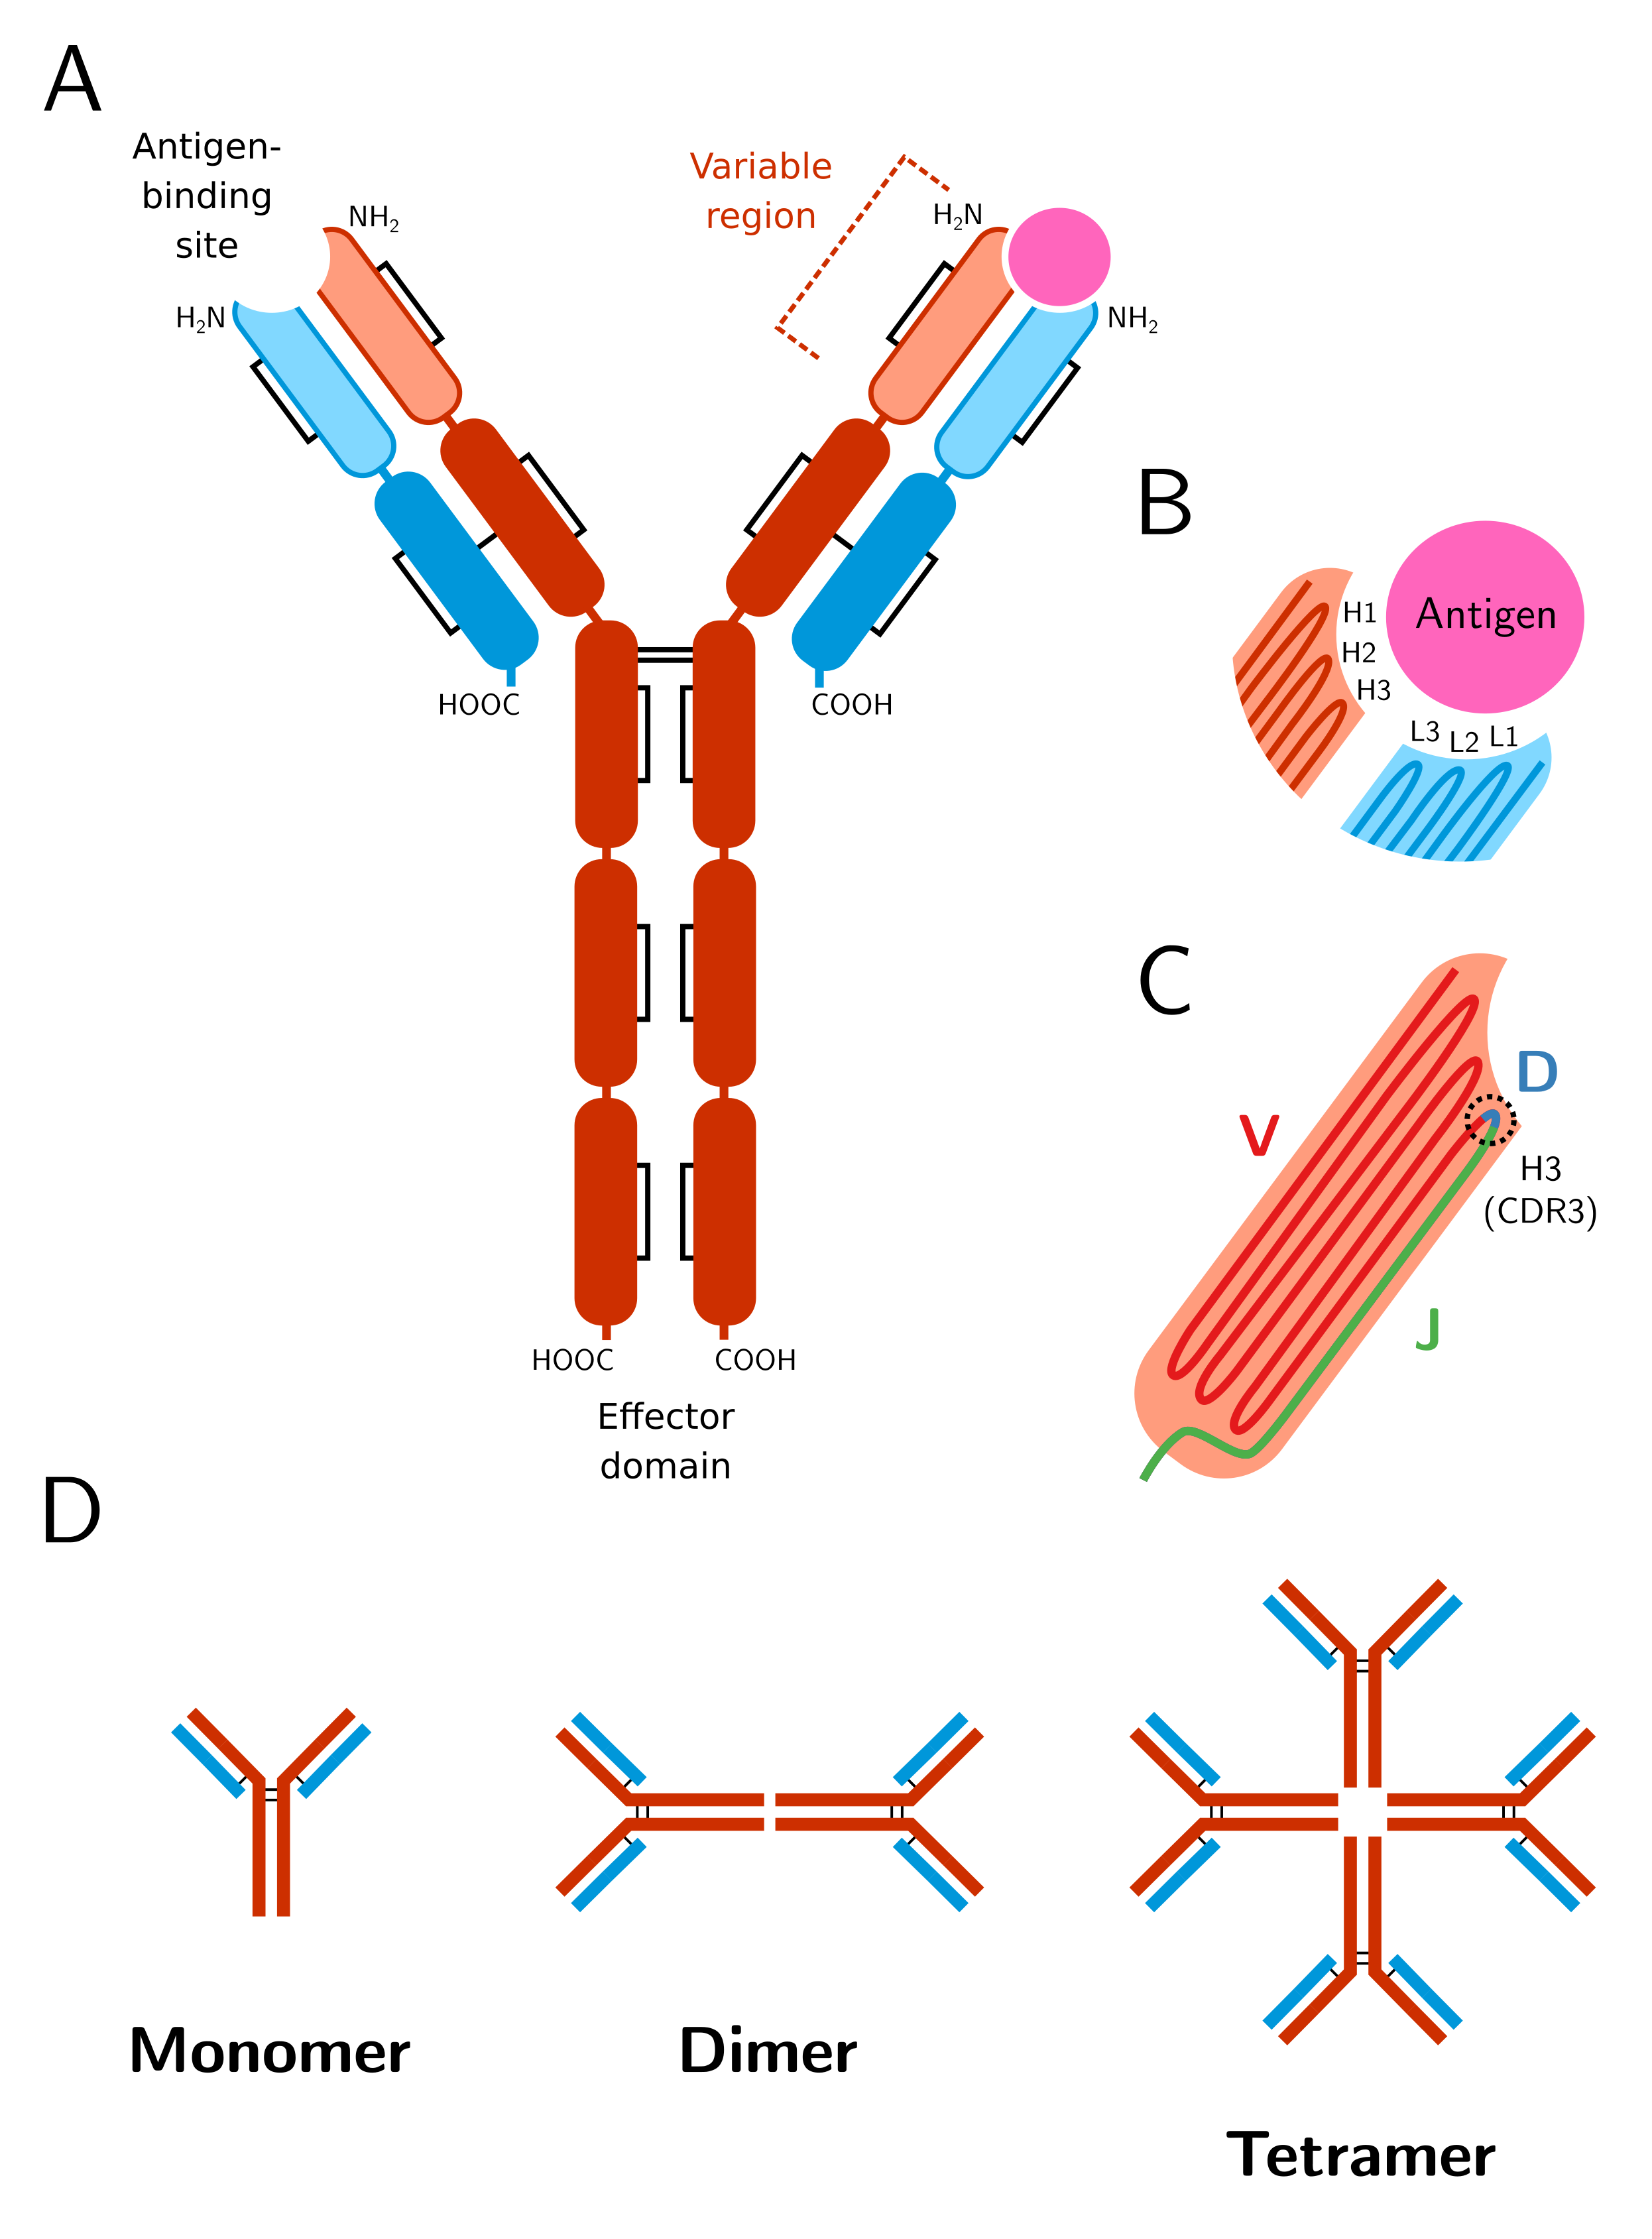
\includegraphics[width=0.9\textwidth]{_Figures/png_edited/antibody-structure}
\begin{subfigure}{0em}
\phantomsubcaption{}
\label{fig:intro-antibody-structure-schematic}
\end{subfigure}
\begin{subfigure}{0em}
\phantomsubcaption{}
\label{fig:intro-antibody-structure-loops}
\end{subfigure}
\begin{subfigure}{0em}
\phantomsubcaption{}
\label{fig:intro-antibody-structure-vdj}
\end{subfigure}
\begin{subfigure}{0em}
\phantomsubcaption{}
\label{fig:intro-antibody-structure-multimers}
\end{subfigure}
\caption[Antibody structure and function]{\textbf{Antibody structure and function:} (A) Schematic of a hingeless secreted antibody monomer, with heavy chains depicted in red, light chains in blue, and bound antigen in pink. Immunoglobulin fold domains are depicted as rounded rectangles, with variable-region domains shown with light shading and constant-region domains with dark. Black lines indicate disulfide bonds. (B) Schematic close-up of an immunoglobulin antigen-binding site, indicating the six loop regions (H1-3 and L1-3) making up the antigen-binding region. (C) Schematic close-up of the heavy-chain variable region, indicating the regions corresponding to the variable, diversity and joining gene segments from the unrecombined \igh{} locus. Note the chimeric nature of the third antigen-binding loop (H3, marked), which is formed by parts of all three gene segments. (D) In the context of antibodies, ``monomer'' refers to a single four-chain antibody protein, while ``dimer'', ``tetramer'' \etc refer to multiple antibodies linked together through covalent or noncovalent interactions.}
\label{fig:intro-antibody-structure}
\end{figure}
% TODO: Actual antibody crystal structure here?

\subsection{Antibody sequence diversification and primary repertoire diversity}
\label{sec:intro_immunity_primary}

% TODO: Discuss allelic exclusion (Magadan)
% TODO: Read up on allelic exclusion in teleosts in Magadan 2015

The immune environment encountered by a vertebrate organism contains an enormous number of different potential pathogenic threats, each of which has its own antigenic signatures and many of which are capable of evolving much more rapidly than the vertebrate host \parencite{jack2015evolution}. In order for the adaptive immune system to cope with this huge diversity of different threats, it must be able to produce antibodies with a correspondingly large diversity of different antigen specificities. The greater the potential diversity of antibody sequences available to the adaptive immune system, the greater its capacity to respond effectively to novel immune threats. In reality, the mechanisms employed by the vertebrate adaptive immune system to diversify its antigen receptors enable an almost unlimited diversity of potential antibody sequences, with a correspondingly vast array of potential antigen specificities \parencite{mora2016quantifying}.

The mechanisms by which the adaptive immune system produces this diversity are dramatic, and rely on a highly unusual underlying gene structure \parencite{jung2006vdjr} and a very high level of cellular wastage \parencite{kogut2012bcells}. In the humoral immune system, antibody diversification takes place during B-cell development in the primary lymphopoietic organs (bone marrow in mammals, anterior kidney in teleosts \parencite{sunyer2013fishing}). Prior to this process, the native antibody loci in B-progenitor cells (and other cell types) is highly fragmented \parencite{jung2006vdjr}, with numerous fragmentary variable-region sequences present in series on the chromosome upstream of the constant-region exons. In the heavy chain locus, these variable-region gene segments can be divided into three categories:

\begin{itemize}
\item \textbf{Variable (\vh) segments} are the longest class of gene segment, at roughly \bp{300} in length. Each V-segment codes for the majority of the variable region of an antibody, including the entirety of the first three framework regions (FWR1-3) and the first two complementarity-determining regions (CDR1-2) as well as the 5' part of CDR3 \parencite{jung2006vdjr} (\Cref{fig:intro-antibody-structure-vdj}). They are therefore highly structured, and include several highly-conserved positions present in virtually all functional V-segments in nearly all species, including two conserved cysteine residues (which code for an intra-domain disulfide bond) and a conserved tryptophan residue following CDR1 \parencite{lefranc2003vnumbering}. Each V-segment is also associated with its own promoter sequence and 5'-UTR, as well as a 5'/C-terminal leader peptide between the translation start site and the start of the functional V-sequence.
\item \textbf{Diversity (\dh) segments} are the shortest class of segment, typically on the order of 10-\bp{20}, and are the least structured \parencite{ruiz1999humandj}. They form the middle part of CDR3 (\Cref{fig:intro-antibody-structure-vdj}) \parencite{schroeder2010immunoglobulins}.
\item \textbf{Joining (\jh) segments} are of intermediate length, typically 50-\bp{60} \parencite{ruiz1999humandj}. They form the 3'/C-terminal part of heavy chain CDR3 and the 5'/N-terminal part of FR4 (\Cref{fig:intro-antibody-structure-vdj}) \parencite{schroeder2010immunoglobulins}. Each J-segment is succeeded on the chromosome by a splice donor site \parencite{magadan2011medaka}, which is used to join the variable region of the antibody sequence to the constant region via RNA splicing following transcription of \igh{} mRNA (\Cref{fig:intro-vdjr-locus}iii). Like \vh segments, \jh segments can be identified from their conserved structure, particularly the conserved tryptophan residue marking the end of CDR3 \parencite{ruiz1999humandj}.
\end{itemize}

In the simplest ``translocon" configuration of the \igh{} locus, blocks of repeated \vh, \dh and \jh segments are present in series on the chromosome in contiguous V-, D- and J-regions (\Cref{fig:intro-vdjr-locus}i) \parencite{schroeder2010immunoglobulins,jung2006vdjr}. During B-cell development, a single \vh, \dh and \jh segment are selected, and the intervening genomic regions are permanently excised from the genome to produce a single contiguous VDJ sequence coding for the complete variable region of an antibody (\Cref{fig:intro-vdjr-locus}ii). The mechanism by which this excision occurs is called VDJ recombination, and relies on a specialised recombinase complex containing lymphocyte-specific recombination-activating genes 1 and 2 (\gene{RAG1} and \gene{RAG2}) \parencite{jung2006vdjr,schatz2011vdjr}. This complex recognises specialised recombination signal sequences (RSSs) flanking each variable gene segment, composed of highly conserved heptamer and nonamer sequences separated by a spacer sequence of conserved length (either 12 or \bp{23}, corresponding respectively to one or two turns of the DNA helix) \parencite{hesse1989rss} (\Cref{fig:intro-vdjr-consensus}). Each functional \vh segment is succeeded by a \bp{23}-spacer RSS in 5'-3' orientation, while each \jh segment is preceded by a \bp{23}-spacer RSS in 3'-5' orientation; each \dh segment, meanwhile, is flanked by \bp{12}-spacer RSSs in 5'-3' and 3'-5' orientation, respectively (\Cref{fig:intro-vdjr-rss}) \parencite{schatz2011vdjr}. 

In VDJ recombination, recombinase complexes bind two of these RSSs and associate with each other to bring the two corresponding gene segments into close proximity (\Cref{fig:intro-vdjr-mechanism}i-iii). A single-strand DNA nick is introduced between each RSS and its gene segment, and the exposed 3'-hydroxyl group of the break attacks the 5'-phosphate on the other strand to produce an asymmetric double-strand break, with the coding sequence terminating in a hairpin loop and the cleaved RSS in a blunt end \parencite{schroeder2010immunoglobulins,schatz2011vdjr} (\Cref{fig:intro-vdjr-mechanism}iv-v). These breaks are then resolved by the ubiquitous non-homologous end-joining machinery of the DNA damage response: the blunt ends of the cleaved RSSs can be directly ligated together, while for the coding sequences the hairpin loops must first be cleaved and the resulting 3'-overhangs resolved \parencite{schroeder2010immunoglobulins,schatz2011vdjr} (\Cref{fig:intro-vdjr-mechanism}vi-vii). The net result of this process is a contiguous V/D or D/J join in the coding sequence and a ligated DNA circle containing the excised RSSs and intervening sequence, which is subsequently degraded. Via unknown mechanisms \parencite{schatz2011vdjr}, the recombination machinery exhibits a strong preference for RSS sequences of different lengths (the so-called ``12/23 rule''), encouraging  D-J and V-D joins while largely preventing V-J joins. 

The simple joining of gene segments during VDJ recombination provides a basic combinatorial sequence diversity, with a number of possible sequences in the simplest case equal to the product of the numbers of \vh, \dh and \jh segments in the \igh{} gene locus. The number of potential \igh{} variable-region sequences in most species, however, is vastly higher than this: in humans, for example, there are roughly 8000 possible functional VDJ combinations \parencite{lefranc2001humanheavy}, but the number of different possible nucleotide sequences exceeds $10^{22}$ \parencite{elhanati2015model}. This huge difference arises from the inexactness with which the coding ends produced by the recombinase complex are joined following RSS excision (\Cref{fig:intro-vdjr-junctions}). Before the two gene segments brought together in VDJ recombination can be joined by NHEJ, the hairpin loops formed by the recombinase complex must be resolved by re-nicking the DNA \parencite{schroeder2010immunoglobulins,schatz2011vdjr}. This re-nicking process is not exact, and often occurs within the coding sequence, resulting in a palindromic 3'-overhang that can be filled in (resulting in palindromic \textit{P-insertions}) or trimmed (resulting in \textit{deletions}). The resulting blunt ends then serve as substrates for the lymphocyte-specific terminal dideoxy transferase enzyme (TdT), which adds a variable number of untemplated nucleotides (nonpalindromic \textit{N-insertions}) prior to sequence ligation \parencite{schroeder2010immunoglobulins,schatz2011vdjr}. As a result, the final recombined sequence is frequently not a clean ligation of the two original gene segments, but an inexact join involving multiple missing terminal positions and/or \textit{de novo} inserted sequence, a phenomenon collectively known as \textit{junctional diversity} (\Cref{fig:intro-vdjr-mechanism}vi-vii) \parencite{flaherty2012chapter}.

The three process contributing to junctional diversity (P insertion, N insertion, and deletion) together vastly increase the potential antibody sequence diversity available to a developing B-cell at the heavy-chain CDR3 region, which as a consequence is by far the most variable single region in determining antigen specificity \parencite{shirai1999h3}. This junctional diversity, however, comes at a substantial cost. The indel mutations introduced by VDJ recombination are not constrained to occur in multiples of three over both junctions, resulting in a high rate of recombinations in which the \vh and \jh segments are out of frame with each other; still more loci are rendered nonfunctional through the introduction of \textit{de novo} STOP codons. As the sequence changes introduced by VDJ recombination are irreversible, many developing B-cells are left with permanently disrupted \igh{} loci on both chromosomes, and are left with no recourse but programmed cell death. In addition, the huge and untemplated sequence diversity introduced in this way means that many B-cells whose \igh{} loci do successfully undergo VDJ recombination are left with BCRs that either cannot effectively bind any antigen or strongly bind self-antigen, resulting in useless antibodies in the first case and a dangerous risk of autoimmunity in the second; these B-cells are eliminated through a process of antigenic selection before \naive B-cells are permitted to exit the primary lymphopoietic organs, resulting in still more wastage as cells with nonfunctional or self-binding antigens undergo programmed cell death. Overall, as many as 90\% of developing B-cells may be eliminated by one or other of these processes before successfully exiting the primary lymphoid organs \parencite{kogut2012bcells}.  

% More details on primary selection in Kogut and its sources if needed

Taken together, the processes of VDJ recombination, junctional diversity and primary selection will produce a population of \naive B-cells with an extremely high diversity of heavy-chain ideotypes, with virtually every \naive B-cell expressing a unique variable-region sequence. Taken together, the resulting population of sequences represents the \textit{primary antibody heavy-chain repertoire} of the organism, and determines the range of different antigen sequences the humoral immune system of that organism can potentially respond to. The diversity of this primary repertoire depends on the native structure of the \igh{} locus in that species (which determines the number of segment choices available to the VDJ-recombination process), the distribution of possible numbers of insertions or deletions contributing to junctional diversity, and the stringency of the primary selection process.

\begin{figure}
\centering
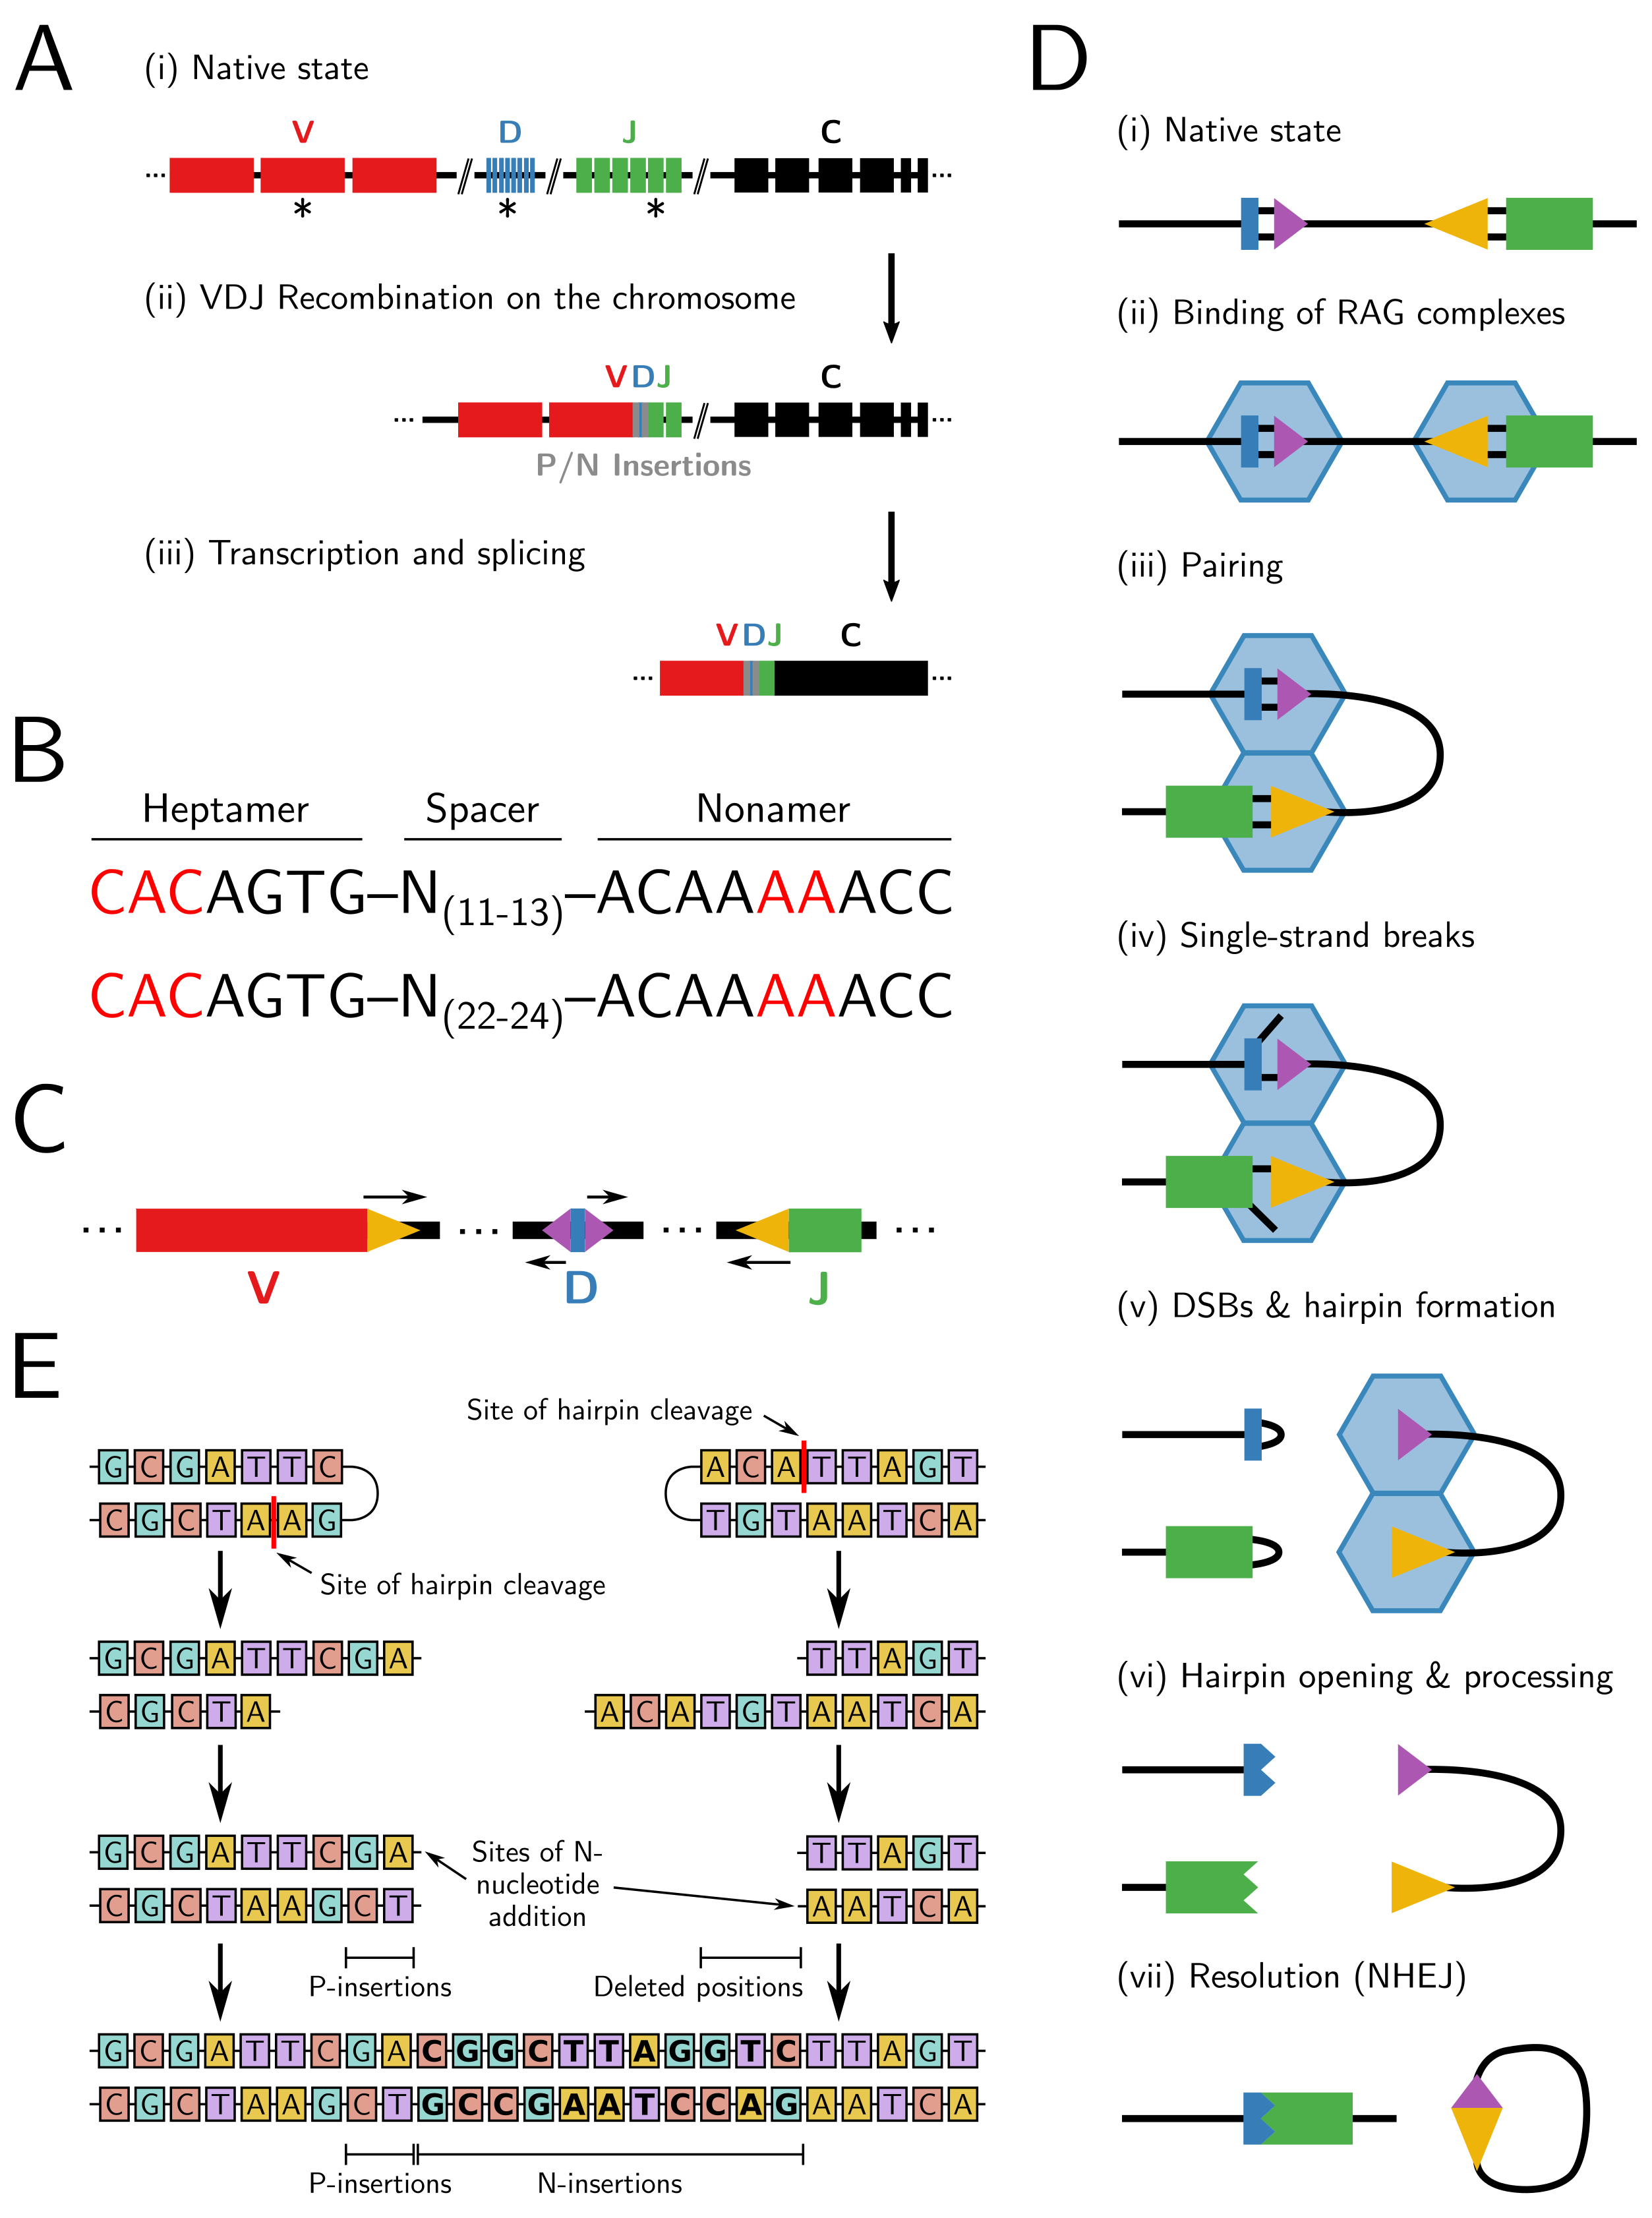
\includegraphics[width=0.95\textwidth]{_Figures/png_edited/primary-diversity}
\begin{subfigure}{0em}
\phantomsubcaption{}
\label{fig:intro-vdjr-locus}
\end{subfigure}
\begin{subfigure}{0em}
\phantomsubcaption{}
\label{fig:intro-vdjr-consensus}
\end{subfigure}
\begin{subfigure}{0em}
\phantomsubcaption{}
\label{fig:intro-vdjr-rss}
\end{subfigure}
\begin{subfigure}{0em}
\phantomsubcaption{}
\label{fig:intro-vdjr-mechanism}
\end{subfigure}
\begin{subfigure}{0em}
\phantomsubcaption{}
\label{fig:intro-vdjr-junctions}
\end{subfigure}
\caption[Primary sequence diversification in antibodies]{\textbf{Primary sequence diversification in antibodies:} (A) Schematic of antibody sequence formation at the locus level. Black asterisks indicate the segments to be recombined. (B) Consensus sequence of short (above) and long (below) RSSs in jawed vertebrates. Nucleotides marked in red are the most strongly conserved and most required for efficient recombination \parencite{hesse1989rss}. (C) Schematic of position and orientation of long (orange) and short (purple) RSSs relative to variable-region gene segments. (D) Schematic of recombination mechanism for a D/J segment pair, illustrating hairpin formation and imprecise end-joining of coding sequences; adapted from \parencite{schatz2011vdjr}, Figure 2. (E) Example of the inexact hairpin resolution mechanisms leading to junctional diversity in (D-vi); adapted from \parencite{flaherty2012chapter}, Figure 10-5.
} 
\label{fig:intro-vdjr}
\end{figure}


%VDJ recombination in the \textit{IGH} locus is highly structured, and occurs in a specific order. First, a D and a J segment are selected and recombined to produce a DJ sequence. Then, a V region is selected and recombined with the DJ to produce a continuous VDJ sequence constituting the variable region of the heavy chain. The complete protein sequence is produced during later transcriptional splicing, which joins this variable-region sequence to downstream constant-region exons to produce a mature \textit{IGH} mRNA. This strict ordering of V/D/J segments, which obtains in the vast majority of recombined sequences observed, is produced through the combination of a variety of regulatory mechanisms. The most basic of these is the structure of the RSSs, which comprise a conserved heptamer and nonamer sequence separated by a relatively unconserved spacer region of either 12 or 23bp \parencite{jung2006vdjr}, corresponding to either one or two turns of the DNA helix. V and J segments in the IGH locus are flanked by RSSs with 23bp spacer regions, while those flanking D-regions have 12bp spacers %citation needed
%As the RAG recombinase specifically recognises pairs of RSSs with dissimilar spacer lengths (a restriction known as the 12/23 or one-turn/two-turn rule), direct V-to-J recombination events are excluded \parencite{jung2006vdjr}. % Better citation if possible.
%
%Complete VDJ recombination places the V-region promoter in close proximity to a highly-conserved enhancer element (known as iE$\mu$) lying between the last J segment and the first constant-region exon \parencite{jung2006vdjr}; this enhancer is important for strong expression of the mature IGH mRNA from the pre-B-cell stage onwards. 

\subsection{\igh{} locus structure in teleost fishes}
\label{sec:intro_teleost_loci}

\Cref{sec:intro_immunity_primary} describes the process of \igh{} locus maturation in terms of an idealised translocon locus with a simple V-D-J-C structure (\Cref{fig:intro-vdjr-locus}). In some species, including humans and mice, \igh{} loci roughly correspond to this simplified structure, albeit with a much larger number of gene segments; however, in many species, including all teleosts, this idealised structure is a significant oversimplification of the actual layout of their \igh{} loci \parencite{fillatreau2013astonishing}. Due to their repetitiveness and complex structure, comprehensive assembly of \igh{} loci is often difficult, and full elucidation of their structure often requires a focused characterisation effort. Nevertheless, a number of teleost loci have been characterised to date, including several species (e.g. three-spined stickleback and medaka) closely related to the African turquoise killifish.

Among teleost fishes, the simplest \igh{} locus structures known to date are exhibited by species such as zebrafish, grasscarp, and fugu (\Cref{fig:intro-teleost-loci-simple}) \parencite{fillatreau2013astonishing}. In these species, the \igh{} locus adopts a V-D-J-\cz{}-D-J-\cm{}-\cd{} structure, with a single shared V-region followed by D- and J-regions specific to the \igh{Z} and \igh{M/D} constant regions, respectively. The rainbow trout locus has a similar organisation, but with two additional V-segments following the \igh{Z} region \parencite{hansen2005trout}. During VDJ recombination in these loci, the choice of variable gene segments also determines the choice of constant region: if a pair of \dh and \jh segments upstream of the \igh{Z} constant region is selected, the cell will express \igh{Z}, while if the segments chosen are downstream of \igh{Z}, that constant region will be excised during VDJ recombination and \igh{M} and/or \igh{D} will be used instead. As a result, VDJ recombination in these species determines both the ideotype of a developing B-cell and its isotype \parencite{fillatreau2013astonishing}.

While some teleost species possess such relatively simple \igh{} loci, many species exhibit much more complicated, and often much larger, locus structures. In many species, multiple distinct subloci (comprising V-, D- and J-regions and least one constant region) are present in tandem on the chromosome, often with distinct combinations of variable gene segments and constant regions (\Cref{fig:intro-teleost-loci-complex}); in a few cases, such as medaka and Atlantic salmon, one or more of these subloci is in inverted orientation relative to the rest of the locus. In some species, such as Atlantic salmon, whole-genome duplication has led to the existence of multiple distinct \igh{} loci on different chromosomes, each of which has its own complement of subloci, gene segments, and constant regions \parencite{yasuike2010salmon}. In this milieu, pseudogenisation of gene segments or constant-region exons is common, resulting in loci with large numbers of pseudogenised V-segments and constant regions.

The diversity in locus size and organisation among teleost fishes is likely to have important consequences for humoral adaptive immunity in these species. The native locus constitutes the raw substrate for the VDJ recombination process, and the number of different \vh, \dh and \jh gene segments available for recombination defines the baseline sequence diversity of antibodies in that species. It is not clear to what extend VDJ recombination can take place across different subloci in the large tandem loci described in \Cref{fig:intro-teleost-loci-complex}; if recombination between subloci is restricted, this will also have important effects on the kinetics of VDJ recombination in a species. The division of an \igh{} locus into tandem subloci may also have effects on the statistics of B-cell maturation, with more subloci conceivably presenting the opportunity for a greater number of recombination attempts before the \igh{} loci of a developing B-cell are exhausted and so reducing the rate at which cells fail to mature successfully; however, to my knowledge little or nothing is known about the effects of locus structure on B-cell developmental processes at present. Finally, variations in the constant regions present in different species are likely to have very important effects on humoral immunity; most fundamentally, whereas \igh{Z/T} appears to be specialised for mucosal adaptive immunity in those teleost species that possess it \parencite{zhang2010igtgut,fillatreau2013astonishing,xu2013igtskin}, it is not known how mucosal immune responses manifest in species lacking this isotype. Given all these important (and potentially-important) effects of \igh{} locus structure on humoral adaptive immunity, characterising the sequence and organisation of this locus is an essential step in understanding the adaptive immune system of any vertebrate species.

\begin{figure}
\centering
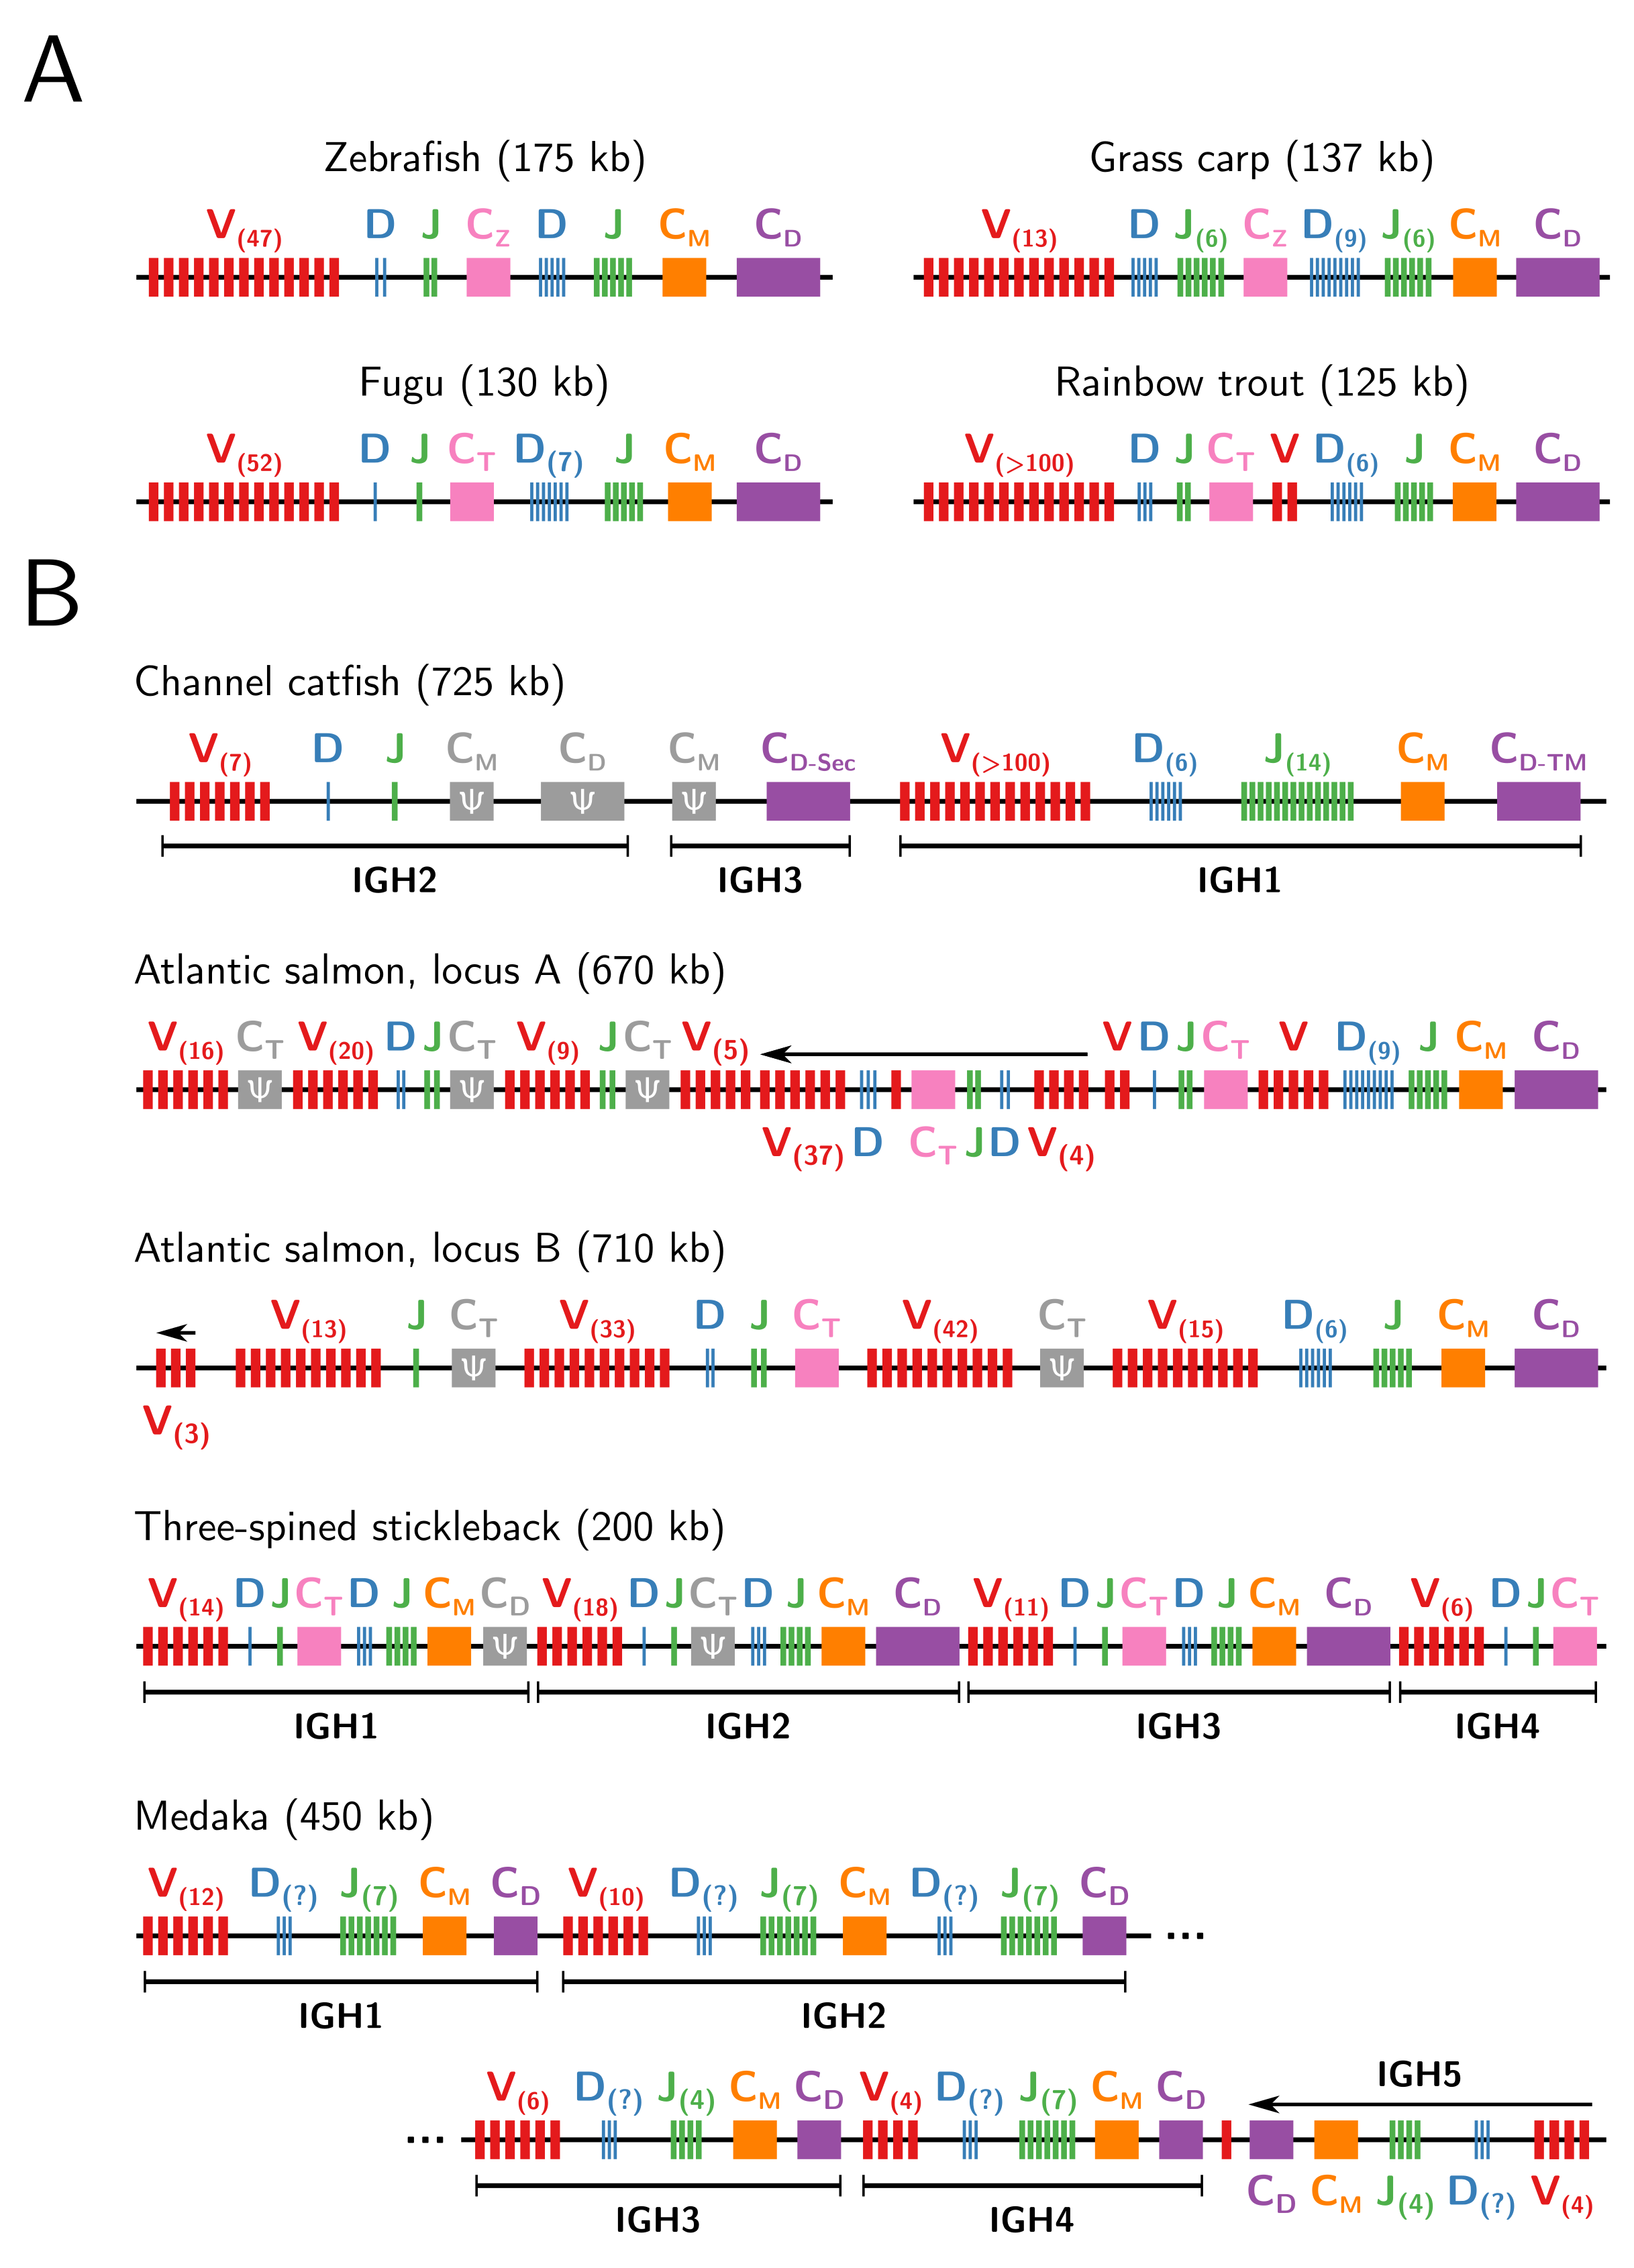
\includegraphics[width=0.85\textwidth]{_Figures/png_edited/teleost-loci}
\begin{subfigure}{0em}
\phantomsubcaption{}
\label{fig:intro-teleost-loci-simple}
\end{subfigure}
\begin{subfigure}{0em}
\phantomsubcaption{}
\label{fig:intro-teleost-loci-complex}
\end{subfigure}
\caption[\igh{} locus structure in teleost fishes]{\textbf{\igh{} locus structure in teleost fishes:} Simplified schematics of \igh{} loci from nine teleost species. (A) In the simplest teleost \igh{} loci, single \igh{Z} and \igh{M/D} constant regions share a common V-region, but are preceded by separate D/J regions. In rainbow trout, a small number of V-segments also separate \igh{Z} from the pre-\igh{M} D-region. (B) In many teleosts, the \igh{} loci are much larger and more complex, with repeated tandem subloci (labelled regions), pseudogenised constant regions (grey, $\psi$), inverted segments (leftward arrows), and other deviations from the classic locus organisation. Loci are not to scale; blocks of more than five segments are condensed and labelled with their segment number, as are some smaller segment blocks for clarity. Adapted from \parencite{fillatreau2013astonishing}, Figure 2 and \parencite{bengten2015fishantibodies}, Figure 4, with additional information from \parencite{magadan2011medaka,bao2010stickleback,gambondeza2011stickleback,yasuike2010salmon,xiao2010grasscarp}.
The number of D-regions in the medaka locus is not provided in the sources.}
\label{fig:intro-teleost-loci}
\end{figure}

\subsection{Affinity maturation and secondary repertoire diversity}
\label{sec:intro_affinity_maturation}

Following VDJ recombination and primary selection, developed \naive B-cells emerge from the primary lymphoid organs and circulate in the periphery. At some point, a subset of these \naive cells will make contact with their cognate antigen. If this contact occurs in the correct signalling context (in particular, in the presence of T-cell help), the B-cell becomes activated and begins to proliferate \parencite{dunnwalters2010bcellageing}. During this clonal expansion process, the B-cell's antibody genes undergo a very high rate of somatic mutation (known as \textit{somatic hypermutation} or SHM), with mutations focused in the complementarity-determining regions coding for the antigen-binding loops of the variable region; in mammals, the rate can be as high as $10^{-3}$ per nucleotide per cell division \parencite{noia2007shm}. This SHM process is orchestrated by the activation-induced cytidine deaminase enzyme (AID), which preferentially targets particular hotspot motifs (canonically  RGYW/WRCY and WA/TW) and deaminates cytidine residues to uracil, which can either be corrected to thymine on DNA replication (resulting in a C-to-T transition mutation) or removed via base-excision repair (resulting in a variety of other mutations) \parencite{magor2015affinity}. As a result, the original antibody sequence of the ancestral \naive cell is diversified into a cluster of related sequences, with widely varying affinity for the cognate antigen.

In order for the combination of clonal expansion and somatic hypermutation to improve the adaptive immune system's ability to respond to the stimulating antigen, the resulting clone needs to undergo a selection process, to identify and advantage cells expressing antibodies with improved antigen affinity. This selection is effected through a competitive process in which clonally-expanded B-cells attempt to bind cognate antigen trapped on the surface of helper cells: those cells which successfully bind antigen receive growth and differentiation signals, while those which do not undergo programmed cell death. In mammals, this process takes place primarily in histologically-distinct germinal centres within specialised secondary lymphoid organs such as the spleen \parencite{howard2006quality,noia2007shm}, in which B-cells that have encountered antigen first undergo clonal expansion and SHM, then compete for antigen on the surface of follicular dendritic cells \parencite{howard2006quality}. In teleosts, which lack specialised, histologically-differentiated germinal centres, B-cell proliferation takes place near clusters of melanomacrophages surrounded by reticular cells, both of which have been attributed an antigen-trapping and -presentation role analogous to that performed by FDCs in mammals \parencite{magor2015affinity}.

While clonal expansion, somatic hypermutation and clonal selection, collectively known as \textit{affinity maturation}, are present in both mammals and teleosts, the increase in antibody affinity resulting from this process in teleosts is far weaker than in mammals (e.g. 3-to-10-fold in rainbow trout, compared to as much as 1000-fold in mammals \parencite{magor2015affinity}). Since SHM appears to be fully functional in those fish so far investigated (albeit with a greater bias towards C-to-T transitions over other mutations) \parencite{magor2015affinity}, this difference seems likely to arise from differences in clonal selection dynamics between teleosts and mammals. The reasons for such a difference are still not entirely clear, but may involve histological differences in where and how affinity maturation takes place in these taxa. In mammalian germinal centres, the ratio between expanded B-cells and FDCs is such that the amount of presenting antigen is limiting, forcing competition for antigen among B-cells and favouring those cells which can bind antigen most strongly \parencite{magor2015affinity}. In teleosts, conversely, proliferating B-cells are far outnumbered by antigen-trapping melanomacrophages and reticular cells, resulting in an oversupply of antigen relative to B-cell demand; this antigen surplus may result in faster overall proliferation, but at the cost of much weaker selection for high-affinity antibodies \parencite{magor2015affinity}.

Following affinity maturation, activated B-cells undergo differentiation into memory cells (which persist in the bloodstream for long periods and provide secondary immune memory) and plasmablasts/plasma cells (which secrete large amounts of antigen to mount a powerful immune response) \parencite{howard2006quality,dunnwalters2010bcellageing}. Affinity-matured cells can also re-enter germinal centres (or their less-developed teleost equivalents) to undergo additional rounds of proliferation, hypermutation and selection \parencite{howard2006quality}; memory cells can also undergo further rounds of affinity maturation, resulting in even larger and more diverse clones and still-higher levels of antigenic affinity. In tetrapods, class switching between different constant-region isotypes also occurs as part of affinity maturation, and is also orchestrated by AID; however, this process is absent in teleosts \parencite{magor2015affinity}.

The combination of the primary (\naive) repertoire described in \Cref{sec:intro_immunity_primary} with the clonal expansions and additional sequence diversity arising from affinity maturation constitutes the \textit{secondary heavy-chain antibody repertoire} of the organism (\Cref{fig:intro-bcell-repertoires}). This is the repertoire actually encountered by incoming pathogens and available to relatively direct experimental interrogation. The structure and diversity of this secondary repertoire depends on the makeup of the primary repertoire, the degree of clonal expansion and hypermutation during affinity maturation, the strength of clonal selection, and the relative abundance of different B-cell subtypes. Inferring the composition of the primary repertoire from that of the secondary is therefore non-trivial, and requires an attempt to distinguish sequences arising from \naive versus activated B-cells or infer the former from the latter; once obtained, the \naive sequences can be used to infer the parameters of the generative process \parencite{elhanati2015model}.

\begin{figure}
\centering
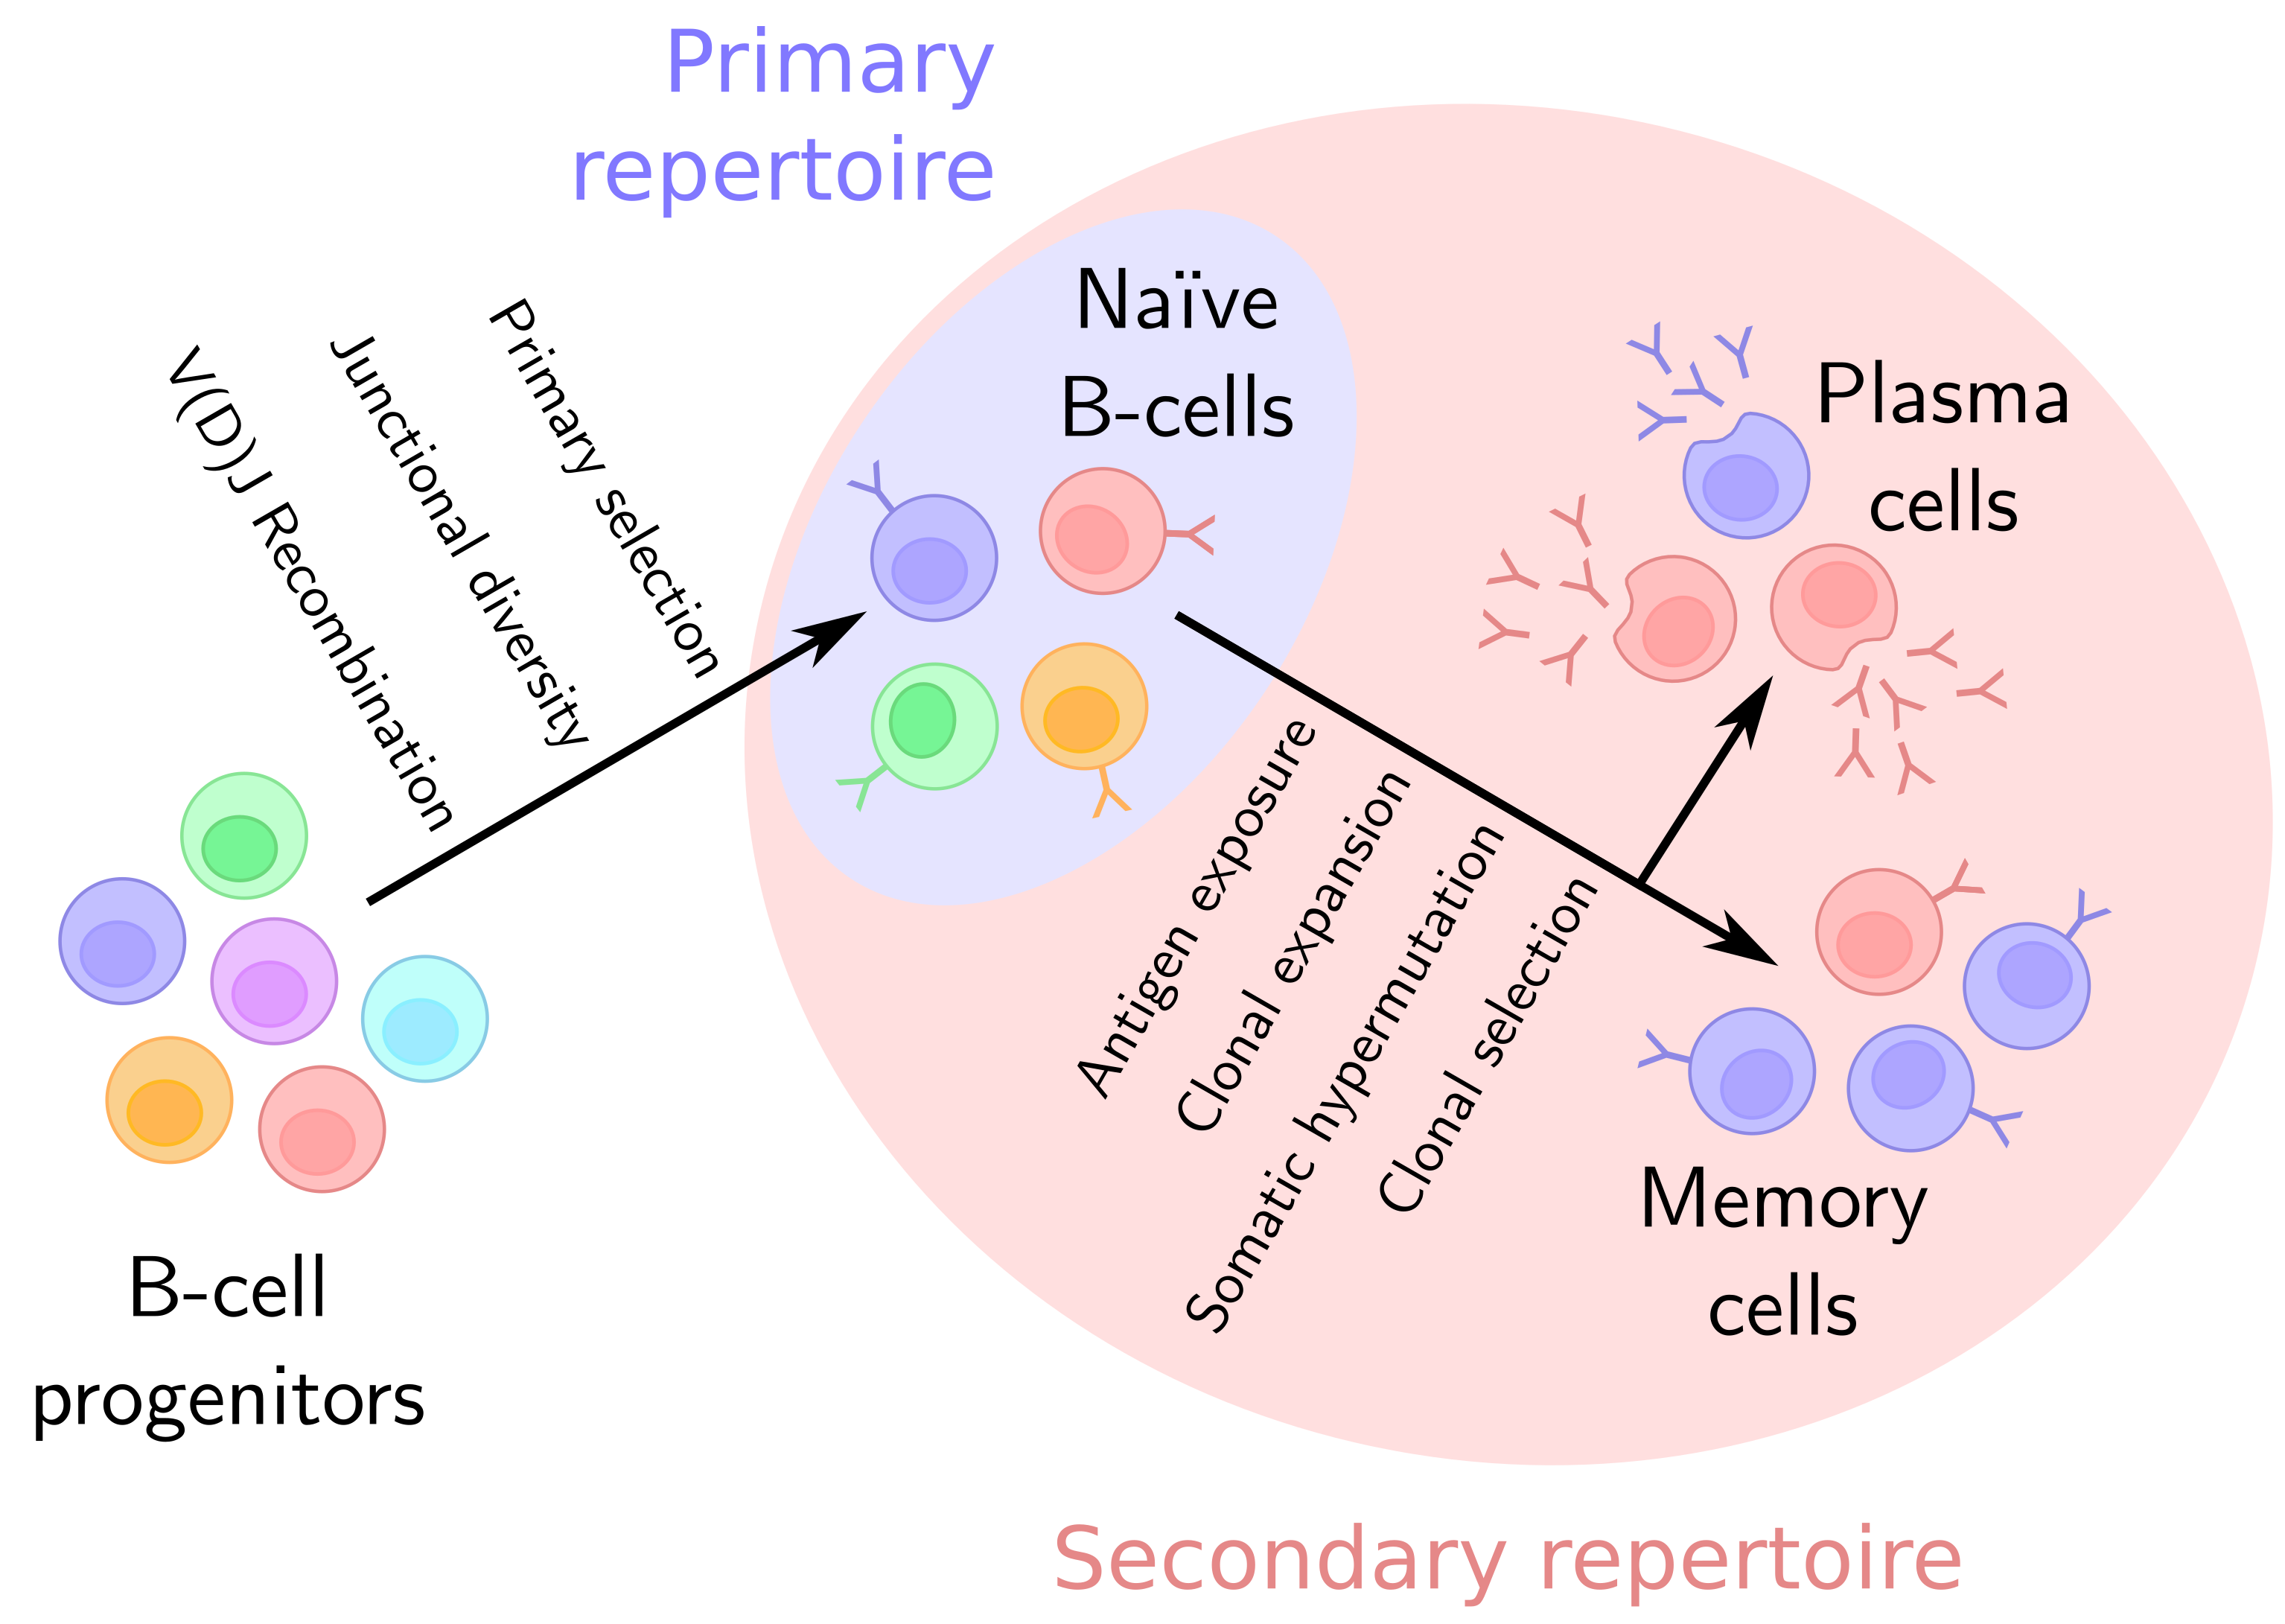
\includegraphics[width=0.9\textwidth]{_Figures/png_edited/bcell-repertoire-primary-secondary}
\caption{\textbf{Primary and secondary antibody repertoires:} Schematic of processes giving rise to the primary (\naive) and secondary (total) B-cell repertoires in the vertebrate immune system. Cell colours indicate clonal membership, with a loss of clonal diversity during primary development (left) and affinity maturation (right). Primary B-cell development (left) takes place in primary lymphoid organs (bone marrow in mammals, anterior kidney in teleosts), while affinity maturation (right) takes place in germinal centres (in mammals) or proto-germinal clusters (in teleosts) in secondary lymphoid organs such as the gut-associated lymphoid tissue (GALT) or spleen.}
\label{fig:intro-bcell-repertoires}
\end{figure}

\section{Humoral adaptive immunosenescence in vertebrates}
\label{sec:intro_immunosenescence}

The immune system of aged vertebrates has long been known to undergo a severe and systemic decline in functionality with age \parencite{segre1977immunosenescence}. As a result of this decline, older individuals exhibit increased susceptibility to a wide range of bacterial, viral, and fungal infectious diseases, as well as higher rates of complications and mortality from those infections when they occur \parencite{sambhara2009vaccination}. In addition, the effectiveness of vaccination against these infections often declines dramatically with age, with older individuals often receiving half or less of the immune protection from vaccination exhibited by younger recipients \parencite{sambhara2009vaccination}. Similar declines in immune functionality with age are also observed in other model organisms, and have been especially well-studied in mice, which share many details of their immune system with humans while being substantially easier to study in depth. While many different parts of the immune system are implicated in this immunosenescent phenotype \parencite{kogut2012bcells}, the decline in the humoral adaptive immune system has emerged as one particularly important contributor \parencite{ademokun2010ageing}.

The changes in the humoral immune system underlying its impaired functionality in old age begin at the level of B-cell development. In mice, the population of haematopoietic stem cells (HSCs) resident in the bone marrow increases in number but exhibits a decreased propensity to regenerate the pool of developing B-cells \parencite{ademokun2010ageing,kogut2012bcells}; factors contributing to this change include a deteriorating bone marrow niche, changes in blood-borne factors affecting HSC differentiation, and the well-known of older mammalian HSCs towards myeloid (rather than lymphoid) cell lineages \parencite{kogut2012bcells,dunnwalters2010bcellageing}. As a result of this change in HSC behaviour, the number of new B-cell progenitor and precursor cells in the bone marrow declines with age in mice; furthermore, these precursors exhibit decreased proliferation capacity, reduced rates of VDJ recombination and an increased rate of apoptosis \parencite{montecino2013immunosenescence,kogut2012bcells,labrie2004bone}. The rate of B-cell output from the bone marrow therefore declines significantly in aged mice compared to young adults, falling as low as 10\% of its level in young mice \parencite{kogut2012bcells}. As these \naive cells also have a shorter lifespan than antigen-experienced memory- and long-lived-plasma-cell populations, the net result of this decline in output from the bone marrow is a decrease in the number of \naive cells in the periphery and a progressive increase in the relative prevalence of antigen-experienced memory and plasma cells \parencite{mehr2011reversing,kogut2012bcells}; the pool of circulating immunoglobulins, meanwhile, becomes progressively dominated by hypermutated antibodies specific to previously-encountered antigens \parencite{kogut2012bcells}. As these \naive cells are essential for responding to novel or mutated immune threats not previously encountered by the immune system, this change is thought to lead to a progressive reduction in the capacity of the humoral immune system to respond effectively to novel threats \parencite{kogut2012bcells}.

Despite the decline in new \naive B-cells produced by the bone marrow, the total number of B-cells in aged mice does not appear to change significantly, reflecting an increase in the absolute number, as well as the relative prevalence, of antigen-experienced B-cell subpopulations. In humans, conversely, the absolute number of total B-cells appears to decline with age \parencite{ademokun2010ageing,montecino2013immunosenescence,aberle2013mechanistic}, with most B-cell subsets showing a significant decline in absolute abundance \parencite{frasca2011age}. Sources differ as to the age-related changes in relative abundance of different B-cell subtypes in humans, with some reporting an increase in the relative prevalence of \naive cells and decrease in that of memory cells\parencite{frasca2011age,blomberg2013age} and others reporting a more mouse-like shift in favour of the memory compartment \parencite{ademokun2010ageing}. These differences may arise from differences in the methods and cell markers used to quantify abundance of different B-cell populations \parencite{ademokun2010ageing}, genuine differences between populations, or the limitations of peripheral blood as a method of sampling the whole-body B-cell population of an individual \parencite{siegrist2009extremes}.

Whatever changes in cellular composition occur in ageing humans, it is clear that both humans and mice undergo a severe age-related decline in B-cell functionality. In humans, the best-understood aspect of this decline is a deterioration in the responsiveness of older patients to vaccination. Older humans frequently exhibit a substantially smaller \parencite{sambhara2009vaccination} and slower \parencite{kogut2012bcells} increase in the titre of antigen-specific serum antibodies in response to vaccination \parencite{sasaki2011limited,aberle2013mechanistic,ademokun2010ageing}, with defects in humoral response observed to vaccines for diseases as diverse as influenza, hepititis A and B, tetanus, diphtheria, pneumococcus and tick-borne encephalitis \parencite{dunnwalters2010bcellageing}. At least in the case of influenza, this decline in specific antibody production is primarily due to a decrease in the number of plasmablasts activated in response to vaccination \parencite{montecino2013immunosenescence,aberle2013mechanistic,sasaki2011limited}.

In addition to being less abundant, the antibodies produced by elderly humans in response to vaccination also appear to be of lower quality: anti-influenza antibodies produced by older human individuals demonstrate reduced ability to effectively neutralise viral haemagglutinin \parencite{kogut2012bcells,sasaki2011limited}, while IGHM antibodies produced by elderly subjects in response to pneumococcal polysaccharide vaccine demonstrate reduced opsonisation ability \parencite{kogut2012bcells}. While basal serum antibody titres actually increase rather than decrease with age in humans and mice \parencite{frasca2009ageing}, suggesting that antibody production \textit{per se} is not impaired with age, these antibodies also decline in quality \parencite{montecino2013immunosenescence}, with measurable increases in the rate of polyspecific and self-reactive antibodies produced in older individuals \parencite{kogut2012bcells}. This decline in baseline antibody quality in older individuals suggests a breakdown in primary B-cell selection in the bone marrow, enabling a greater number B-cells with low-specificity or self-reactive antibody sequences to emerge into the periphery \parencite{ademokun2010ageing}.

Various aspects of affinity maturation are also impaired in aged mammalian B-cells. While memory-cell clones established early in life often persist into old age, \naive B-cells in aged humans demonstrate a severely reduced ability to give rise to new antigen-specific memory B-cells following antigenic stimulation, impairing the establishment of functional immune memory for novel threats \parencite{aberle2013mechanistic}. B-cells from older humans and mice also exhibit impaired class-switch recombination capacity, possibly as a result of decreased AID expression \parencite{montecino2013immunosenescence,blomberg2013age,frasca2011age}, impairing the generation of antibodies with the same specificity but different effector functions. The decreased ability of older individuals to produce high-affinity antigen-specific antibodies \parencite{frasca2011age} also suggests a defect in affinity maturation, though this could also be attributable to the known ageing-related defects in the T-helper and follicular dendritic cells involved in secondary B-cell selection \parencite{montecino2013immunosenescence,aberle2013mechanistic,ademokun2010ageing} rather than changes in the B-cells themselves. Conversely, the effect of ageing on the somatic hypermutation process remains controversial \parencite{henry2019influenza,howard2006quality,ademokun2010ageing,frasca2009ageing}, with different groups reporting an increase, a decrease, or no change in the rate and level of SHM accumulation of different B-cell subtypes with age. 

The various cellular and population-level changes that occur in the humoral immune system with age naturally have important effects on the antibody repertoires of ageing individuals. Aged humans \parencite{siegrist2009extremes} and mice \parencite{dunnwalters2010bcellageing} exhibit increased rates of non-malignant clonal expansions in the memory-cell compartment, which when combined with the apparent maintenance or decline in total B-cell number would lead to a reduction in overall diversity \parencite{dunnwalters2010bcellageing}. Similarly, early techniques that investigated the repertoire by investigating the distribution of CDR3 lengths (CDR3 spetratyping) indicated that older humans frequently exhibit more distorted distributions dominated by CDR3 regions of a particular length, indicative of clonal expansion, and found that older individuals with more distorted spectratypes exhibited greater frailty and worse health and lifespan outcomes than those with more young-like spectratypes \parencite{gibson2009spectratyping}. On the basis of these and similar findings, the antibody repertoire has long been thought to decline in diversity in older individuals, impairing the adaptability of the ageing adaptive immune system.

More recently, the development of specialised high-throughput-sequencing-based techniques for interrogating antibody repertoires (\Igseq, or \igseq \parencite{weinstein2009igseq}) has enabled a few studies to investigate the ageing of these repertoires in greater detail. These studies, primarily on human peripheral blood, have confirmed many observations made using older lower-throughput methods: a reduced number of clonal lineages in older repertoires reflects decreased \naive-cell output from the bone marrow) \parencite{jiang2013vaccine}, while an increase in mean CDR3 length \parencite{wang2014ageing} and the average rate of premature STOP codons \parencite{debourcy2017ageing} in older repertoires similarly support the finding that primary and clonal selection are impaired with age. 
An increase in clonal expansion in older individuals is also observed: 
an \textit{oligoclonal} phenotype, in which one or a few large clones dominate the repertoire, is often seen in peripheral blood from elderly humans but very rarely in the young \parencite{wang2014ageing,debourcy2017ageing}. These expanded clones are persistent before and after vaccination \parencite{debourcy2017ageing} and even across multiple years \parencite{wang2014ageing}; in contrast, large clones observed in young human blood repertoires are typically transient responses to recent antigen challenge \parencite{wang2014ageing}.

The reduction in clonal richness and increase in clonal expansions seen in older individuals contribute to an overall reduction in the estimated number of unique sequences present in the peripheral repertoire \parencite{debourcy2017ageing}, a change observed for both \naive and mutated sequences and exacerbated by a significant reduction in within-clone sequence diversity in at least some elderly individuals \parencite{debourcy2017ageing}. The same study also found a drop in the percentage of unique sequences identified as coming from \naive B-cells, suggesting a mouse-like shift in repertoire prevalence towards antigen-experienced cell types \parencite{debourcy2017ageing}. However, while the alpha (within-individual) sequence diversity of the human peripheral repertoire appears to decline with age, the beta (between-individual) diversity of the repertoire actually increases, with repertoires from older individuals differing more from one another than those of young individuals \parencite{debourcy2017ageing}. Elderly repertoires also showed decreased flexibility in response to immune challenge, with repertoires taken from the same individual pre- and post-vaccination being significantly more similar in elderly than in young samples \parencite{debourcy2017ageing}, perhaps as a result of longer and more individualised histories of antigen exposure. Taken together, these findings suggest a pattern in which human peripheral antibody repertoires progressively lose diversity of the course of the human lifespan, while also becoming increasingly individualised and distinct.

In conclusion, there is strong evidence for a variety of developmental and physiological changes in the B-cell immune system with age in both mice and humans, giving rise to a severe decline in overall functional performance and immune protection. Many of these changes affect the composition of the antibody repertoire, with a reduction in clonal and sequence diversity and an increase in between-individual variability with age in human blood. However, despite this abundance of data, there remain some serious limitations in our knowledge of the ageing antibody repertoire.  From an evolutionary and comparative perspective, almost nothing is known about adaptive immunosenescence in species other than humans and mice; while several \igseq studies have been performed on teleost fish \parencite{weinstein2009igseq,jiang2011determinism,krasnov2017igseq,lund2019salmon,fu2018fugu}, for example, none to my knowledge have investigated B-cell immunosenescence in this taxon. Many of the findings reported above are specific to IGHG or IGHA antibodies in mice and humans \parencite{kogut2012bcells}, and may not generalise to species lacking these isotypes. Even in humans, the majority of immunosenescence studies, including virtually all repertoire studies, are limited to peripheral blood, and therefore primarily sample the minority of B-cells in transition between tissues; the majority of B-cells, which are resident in some immune organ or tissue, are systematically underrepresented in these samples \parencite{siegrist2009extremes,tabibiankeissar2016ageing}. Relatively little is therefore known about how the ageing of the B-cell repertoire differs between organs; the only paper I know of which investigated changes in antibody-repertoire diversity with age in biopsies from multiple human tissues failed to find any significant changes in alpha diversity, except for a significant \textit{increase} in repertoire sequence entropy in old spleen \parencite{tabibiankeissar2016ageing}. No published paper I know of has yet to investigate the ageing of the antibody repertoire at mucosal surfaces, where secreted antibodies play a particularly important role in regulating microbiotal communities and defending the body from pathogenic invasion.

In addition to this lack of spatial resolution in our knowledge of antibody repertoire ageing, there is a serious lack of temporal resolution; most studies of antibody repertoire ageing simply compare a ``young'' group (say 20-30 years of age) with one or two ``old'' groups (say $\geq70$ years of age), with little or no information about the intervening progression of any observed phenotypes \parencite{debourcy2017ageing,tabibiankeissar2016ageing}. The effect of known lifespan-increasing interventions on immune repertoire ageing also remains largely unstudied. Due to their very long lifespans and restrictions on experimental manipulation, humans are unsuitable subjects for these sorts of experiments, as are long-lived vertebrate model organisms such as zebrafish (median lifespan c. 3.5 years \parencite{gerhard2002zebrafish}) and \textit{Xenopus} (median lifespan c. 9 years \parencite{bowler1977longevity}). Even mice (median lifespan c. 2 to 2.5 years for the most common laboratory strains \parencite{yuan2009aging}), though widely used in biogerontology, are inconveniently long-lived for many ageing experiments. Conversely, many major model organisms in ageing research (such as fruit flies and nematode worms) are invertebrates, and so lack a mammal-like adaptive immune system. The development of a short-lived vertebrate species as a model organism for antibody-repertoire experiments would therefore be highly valuable for immunosenescence research, as well as ageing research more generally.

\section{The African turquoise killifish as a model for vertebrate ageing}
\label{sec:intro_killifish}

The genus \textit{Nothobranchius} comprises a broad group of annual freshwater fishes distributed across equatorial and subequatorial Africa \parencite{valdesalici2003lifespan}, with species diversity concentrated in the south-east of the continent \parencite{genade2005annual}. Members of this genus share a suite of adaptations to life in ephemeral pools and rivers, most notably the production of desiccation-resistant embryos capable of surviving through the dry season in a diapause state \parencite{genade2005annual}. Fish from this genus have been known for several decades to  exhibit very rapid growth and short lifespans, consistent with their evolving under conditions of very high extrinsic mortality \parencite{valdesalici2003lifespan}, with many species exhibiting a median lifespan of less than one year. Nevertheless, there is wide variation within the genus in body size, growth rate and lifespan, with species from less arid regions tending to show slower growth and longer median lifespans \parencite{genade2005annual}.

Like other \textit{Nothobranchius} species, the turquoise killifish (\nfu) is a medium-sized annual fish first isolated from ephemeral freshwater pools -- in this case, from a relatively arid region of southeastern Zimbabwe \parencite{genade2005annual,jubb1971new}. Even by the standards of the \textit{Nothobranchius} genus, \Nfu exhibits extremely rapid growth, maturation, and ageing, with the most widely-used laboratory strain (GRZ) exhibiting a median lifespan of just 9-16 weeks \parencite{valdesalici2003lifespan,genade2005annual,terzibasi2008strains,kirschner2012map,valenzano2015genome,smith2017microbiota} -- the shortest lifespan of any captive-bred vertebrate, and a dramatic outlier on the distribution of vertebrate lifespans. Combined with their possession of several important vertebrate-specific adaptations -- including an adaptive immune system -- this extremely short lifespan makes the turquoise killifish a highly promising model organism for ageing research \parencite{harel2015crispr}.

Despite its very short lifespan, \textit{N. furzeri} has been found to show a wide range of senescent phenotypes in even the shortest-lived strains, including lipofuscin deposition \parencite{genade2005annual};  accumulation of senescence markers \parencite{genade2005annual};  increased neurodegenaration \parencite{valenzano2006resveratrol1,valenzano2006resveratrol2}; impaired learning and behavioural phenotypes  \parencite{genade2005annual,valenzano2006resveratrol1}; and a high incidence of degenerative and neoplastic lesions \parencite{dicicco2011histopathology}. These diverse phenotypes indicate that the short lifespan of the turquoise killifish is the result of an accelerated general ageing process, rather than the specific failure of a particular organ or system. Moreover, established anti-ageing interventions such as resveratrol treatment \parencite{valenzano2006resveratrol1}, reduction in ambient temperature \parencite{valenzano2006temperature} and dietary restriction \parencite{terzibasi2009dr} also extend lifespan in the turquoise killifish, indicating a strong analogy with the ageing phenotypes observed in canonical model systems.

Due primarily to its potential as a model organism for ageing research, the turquoise killifish has also seen rapid development as a genetic model. The short-lived GRZ strain has been bred in captivity for fifty years and at least a hundred generations \parencite{terzibasi2007review} and exibits a very high degree of homozygosity \parencite{kirschner2012map,reichwald2009genome,valenzano2009map}, providing a uniform genetic background for experimental interventions. A number of important genetic resources are now available, including several assemblies of the nuclear genome \parencite{reichwald2015genome,valenzano2015genome,willemsen2019popgen}, the most recent of which (\parencite{willemsen2019popgen}, in preparation) is of very high quality. These assemblies have yielded a genome with an estimated size of roughly 1.5 gigabases \parencite{willemsen2019popgen};
karyotyping \parencite{reichwald2009genome} and sequencing analysis \parencite{reichwald2015genome} both indicate a chromosome number of $2n = 38$, corresponding to 19 distinct linkage groups in the haploid genome.

Prior to the work contained in this thesis, almost nothing was known about the adaptive immune system of the turquoise killifish. However, as a teleost, and therefore as a jawed vertebrate, it could be strongly expected to have a roughly mammal-like adaptive immune system, and a number of genes related to B-cell adaptive immunity (including \gene{RAG1}, various B-cell developmental markers, and fragments of antibody genes) were identified in one or more genome annotations. Phylogenetically, the genus \textit{Nothobranchius} falls within the Cyprinodontiformes, and the turquoise killifish is therefore relatively closely related to several species with previously-characterised \igh{} loci, including fugu, stickleback and medaka \parencite{terzibasi2007review,hughes2018teleostphylo}. Despite the relatively unknown state of adaptive immunity in the turquoise killifish, therefore, there was good reason to believe it possessed a functional B-cell immune system similar to those of other teleosts, and therefore comparable in many respects with those of mammalian species, including humans. When combined with its short lifespan and rapid ageing phenotype, this makes the turquoise killifish a potentially highly-valuable model for studying the forms and mechanisms of humoral adaptive immunosenescence in jawed vertebrates. In this thesis, therefore, I characterised the \igh{} locus of the turquoise killifish, established a working \igseq protocol, and performed the first experiments investigating adaptive immunosenescence in this species.

\begin{figure}
\centering
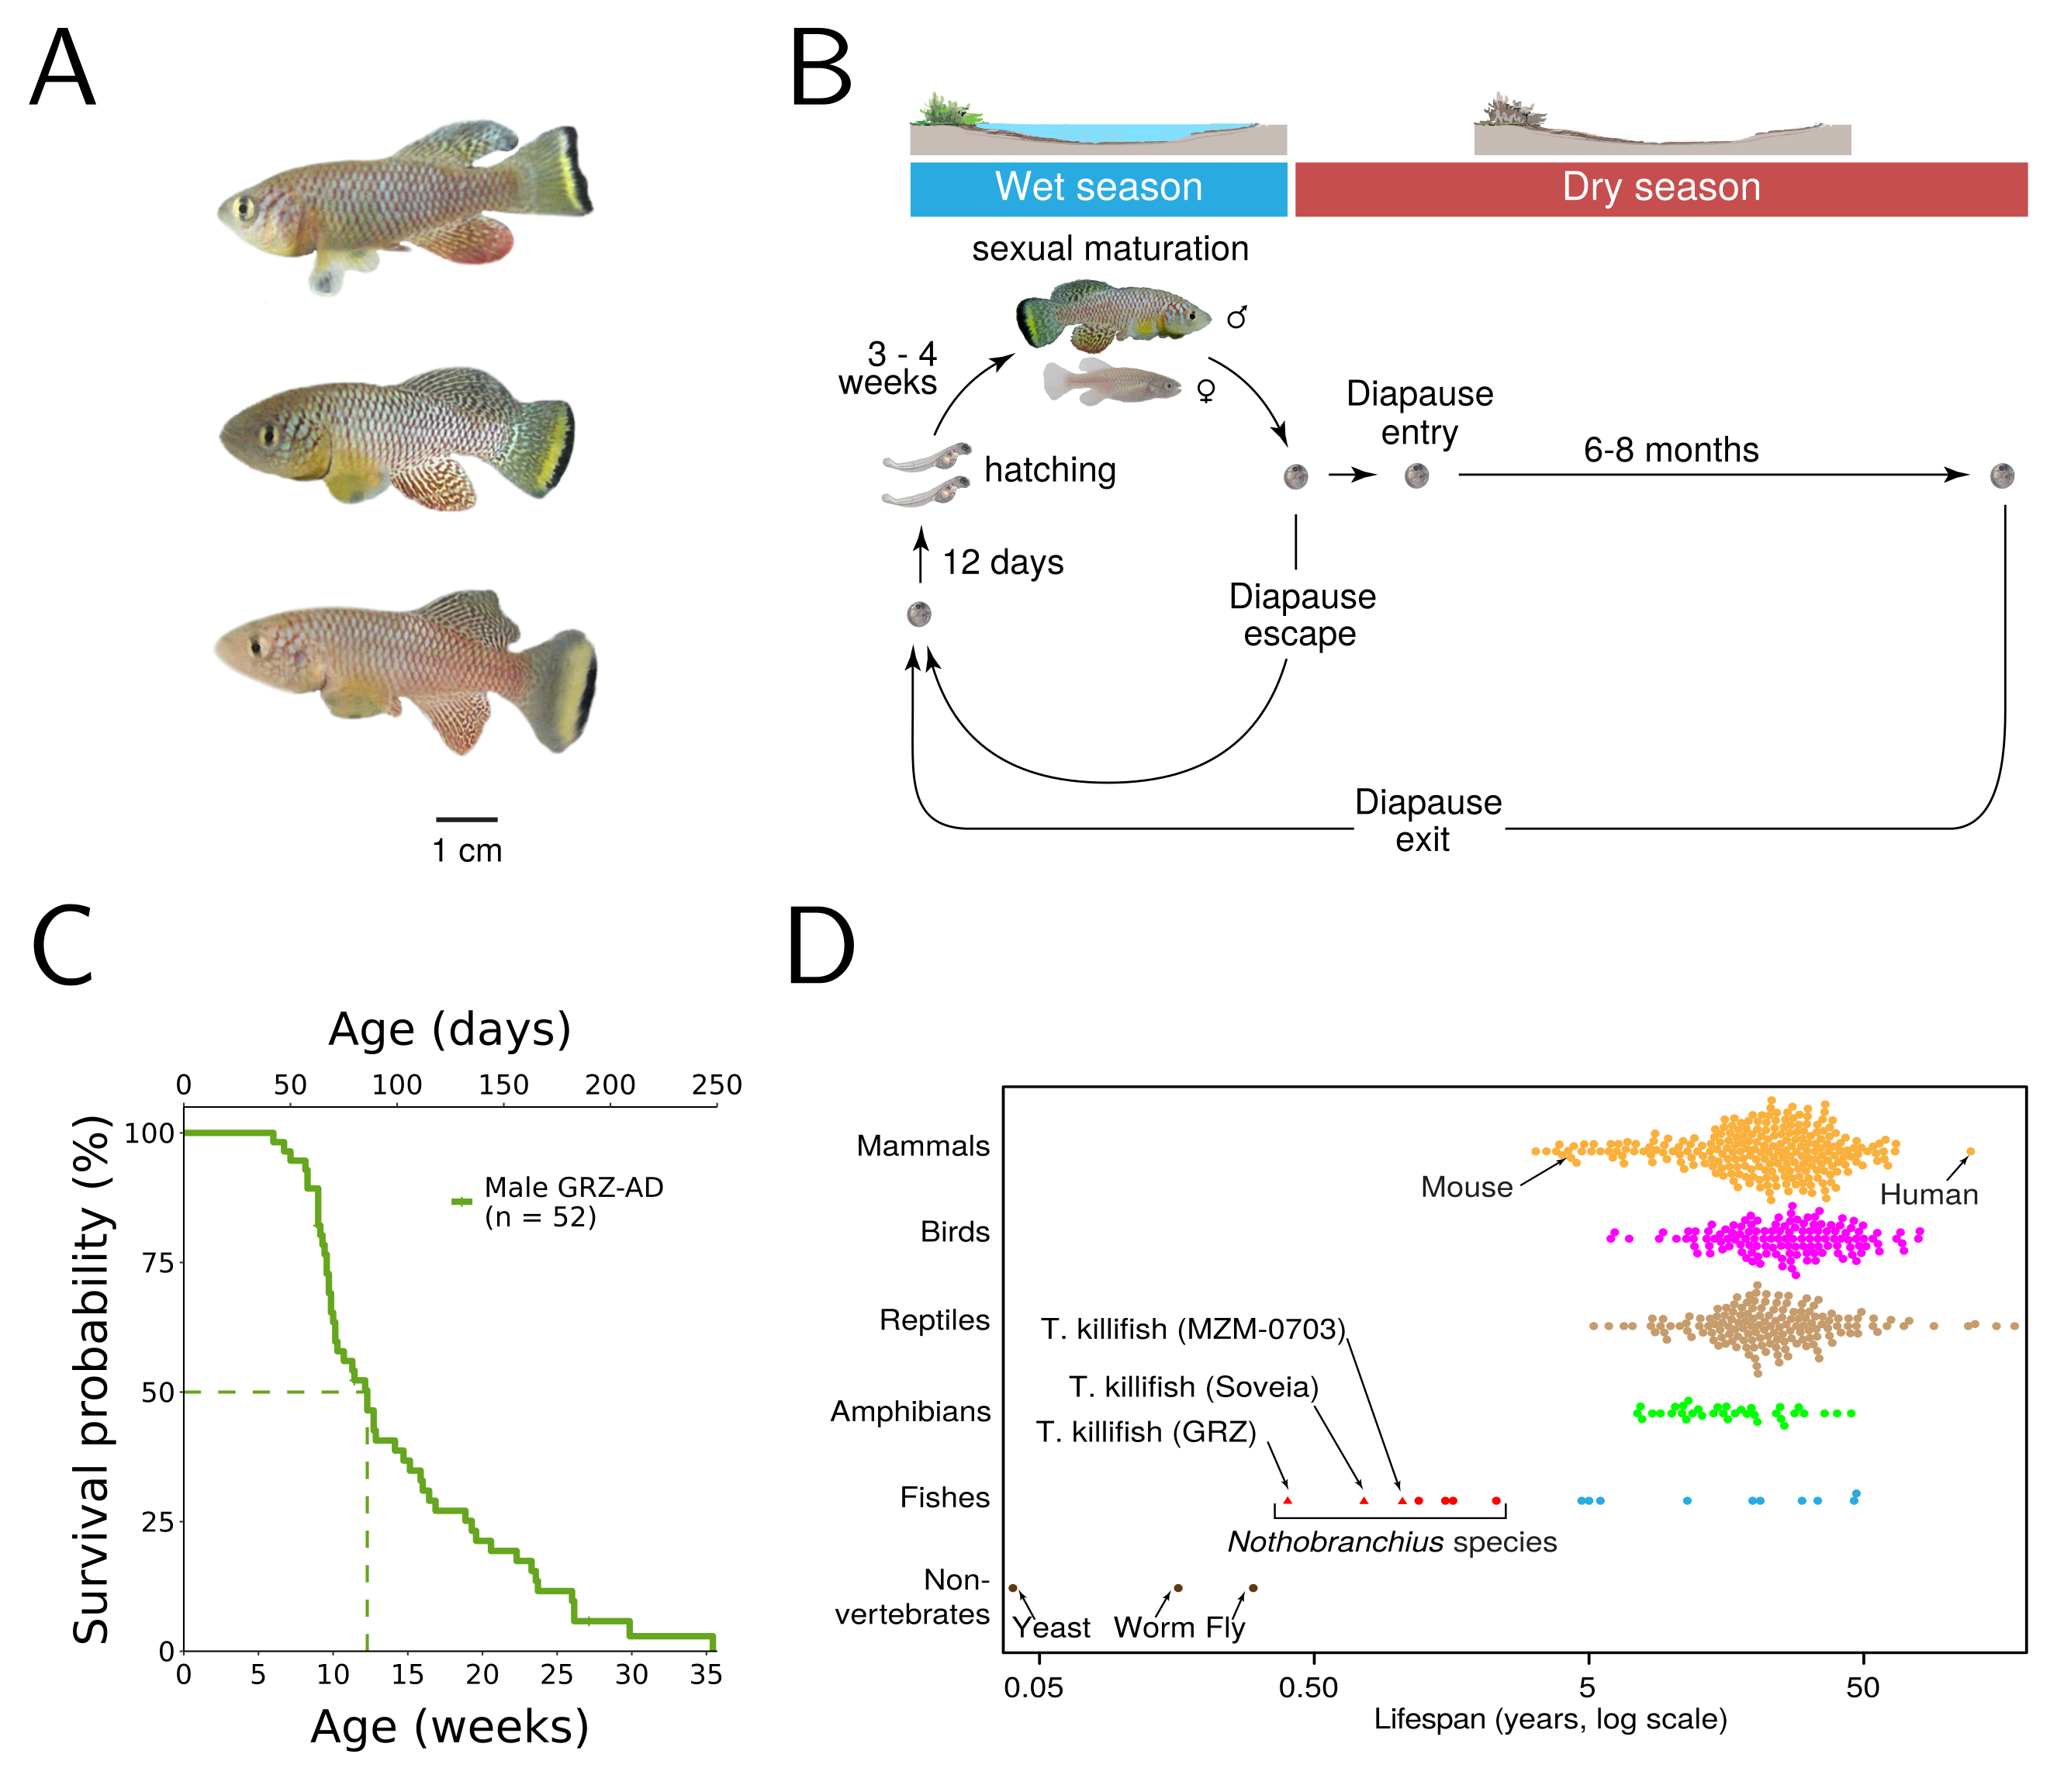
\includegraphics[width=0.95\textwidth]{_Figures/png_edited/intro-turquoise-killifish}
\caption[The turquoise killifish (\nfu) as a model for vertebrate ageing]{\textbf{The turquoise killifish (\nfu) as a model for vertebrate ageing:} (A) Photographs of adult male yellow-tailed turquoise killifish.
(B) Life cycle of the turquoise killifish in its natural environment, showing hatching and breeding during the rainy season and embryo survival in diapause during the dry season.
(C) Example lifespan curve of short-lived GRZ-AD turquoise-killifish males, hatched in December 2016, with a median lifespan of roughly 12 weeks.
(D) Comparison of turquoise-killifish maximum lifespan (red triangles) to other vertebrate species, demonstrating the extremely short lifespan of \Nfu compared to other vertebrates. (A), (B) and (D) adapted from \parencite{valenzano2015genome}, Figure 1.}
\end{figure}
%!TEX root = ../thesis.tex
% TODO: Change this?

\chapter{Materials and methods}  
\onehalfspacing

\pagebreak

%%%%%%%%%%%%%%%%%%%%%%%%%%%%%%%%%%%%%%%%%%%%%%%%%%%%%%%%%%%%%%%%%%%%%%%%%%%%%%%
% FISH HUSBANDRY SECTION
%%%%%%%%%%%%%%%%%%%%%%%%%%%%%%%%%%%%%%%%%%%%%%%%%%%%%%%%%%%%%%%%%%%%%%%%%%%%%%%

\section{Killifish husbandry and sample preparation methods}
\label{sec:methods_husbandry}

Male turquoise killifish (\nfu, GRZ-AD strain) from a single hatching were raised under standard husbandry conditions \parencite{dodzian2018husbandry} and housed from four weeks post-hatching in individual \lt{2.8} tanks connected to a water recirculation system. Fish received \hr{12} of light per day on a regular light/dark cycle, and were fed blood
worm larvae and brine shrimp nauplii twice a day during the week and once a day during the weekend \parencite{dodzian2018husbandry,smith2017microbiota}.

Sacrificed fish (\Cref{tab:igseq-cohorts-fish}) were killed by anaesthetisation in \gl{1.5} Tricaine solution in room-temperature tank water \parencite{carter2011tricaine}, then flash-frozen in liquid nitrogen and ground to a homogenous powder with a pestle in a liquid-nitrogen-filled mortar. The powder was mixed thoroughly and stored at \degC{-80} prior to RNA isolation.

%%%%%%%%%%%%%%%%%%%%%%%%%%%%%%%%%%%%%%%%%%%%%%%%%%%%%%%%%%%%%%%%%%%%%%%%%%%%%%%
% MOLECULAR/WETLAB SECTION
%%%%%%%%%%%%%%%%%%%%%%%%%%%%%%%%%%%%%%%%%%%%%%%%%%%%%%%%%%%%%%%%%%%%%%%%%%%%%%%

\section{Biochemistry and molecular biology methods}

\subsection{Standard methods}

\subsubsection{PCR}
\label{sec:methods_molec_standard_pcr}

The polymerase chain reaction is a well-established method for rapid amplification of a DNA sequence through repeated cycles of denaturation, priming and replication by a high-temperature-tolerant DNA polymerase enzyme \parencite{paul2010hotstartpcr}. Unless otherwise specified, all PCRs in this chapter were performed using \x{2} Kapa HiFi HotStart ReadyMix PCR Kit (\Cref{app:solutions_enzymes}) according to the manufacturer's instructions. Briefly, for a \ul{25} reaction, \ul{12.5} Kapa ReadyMix was combined with \ul{12.5} total of template, nuclease-free water, and primers; these volumes were scaled linearly for reactions of different volumes. The mixture was then heated in a thermocycler as follows:

\begin{center}
\begin{threeparttable}
\begin{tabular}{cccc}\toprule
\textbf{Step} & \textbf{Temperature [\degC{}]} & \textbf{Duration [\secs{}]} & \textbf{Cycles}\\\midrule
Initial denaturation & 95 & 180 & 1 \\\midrule
Denaturation & 98 & 20 & \multirow{3}{*}{$n_c$\tnote{a}}\\
Annealing & $T_a$\tnote{a} \tnote{} & 15 & \\
Extension & 72 & $t_{ext}$\tnote{a} & \\\midrule
Final extension & 72 & $t_{ext} \times 4$\tnote{a} & 1\\
\bottomrule\end{tabular}
\begin{tablenotes}
\item[a] Annealing temperature ($T_a$), extension time ($t_{ext}$) and cycle number ($n_c$) determined separately for each reaction.
\end{tablenotes}
\end{threeparttable}
\end{center}

\subsubsection{Nucleic-acid purification with SeraSure magnetic beads}
\label{sec:methods_molec_standard_serasure}

Nucleic-acid isolation, size-selection and concentration in the \igseq library preparation protocol (and elsewhere where necessary) was performed using SeraSure SPRI (solid phase reversible immobilization) bead preparations \parencite{hawkins1994spri,deangelis1995spri,lennon2010cleanup,fisher2011cleanup}. In SPRI, paramagnetic beads bind DNA in the presence of polyethylene glycol (PEG), with the affinity of the beads for DNA depending on the concentration of PEG in the binding buffer. As a result, the range of nucleic-acid sequence lengths retained by SPRI bead purification depends primarily on the concentration of PEG, which in turn depends on the relative volume of SeraSure bead suspension added to a sample; the higher the concentration, the shorter the minimum fragment length retained during the purification process. In combination with a magnetic rack to remove the DNA-bound beads from suspension, this allows DNA of the desired size range to be isolated from a solution and resuspended in the desired volume of fresh buffer.

To prepare \ml{50} of SeraSure bead suspension for DNA (or DNA:RNA heteroduplex) isolation, a stock of SeraMag beads (\Cref{app:solutions_reagents}) was vortexed thoroughly, then \ml{1} was transferred to a new tube. This tube was then transferred to a magnetic rack and incubated at room temperature for \mins{1}, then the supernatant was removed and replaced with \ml{1} TET buffer (\Cref{app:solutions_buffers}) and the tube was removed from the rack and vortexed thoroughly. This washing process was repeated twice more, for a total of three washes in TET. A fourth cycle was used to replace the TET with incomplete SeraBind buffer (iSB, \Cref{app:solutions_buffers}). The vortexed \ml{1} aliquot of beads in iSB was then transferred to a conical tube containing \ml{28} iSB and mixed by inversion. To add the PEG, \ml{20} \pc{50} (w/v) PEG 8000 solution was dispensed slowly down the side of the conical tube, bringing the total volume to \ml{49}. Finally, this was brought to \ml{50} by adding \ul{250} \pc{10} (w/v) Tween 20 solution and \ul{750} autoclaved water to complete the SeraSure bead suspension.

To perform a bead cleanup, an aliquot of prepared SeraBind solution was vortexed thoroughly to completely resuspend the beads, then the appropriate relative volume of SeraSure suspension was added to a sample, mixing thoroughly by gentle pipetting. The sample was incubated at room temperature for \mins{5} to allow the beads to bind the DNA, then transferred to a magnetic rack and incubated for a further \mins{5} to draw as many beads as possible out of suspension. The supernatant was removed and discarded and replaced with \pc{80} ethanol, to a volume sufficient to completely submerge the bead pellet. The sample was incubated for 0.5-\mins{1}, then the ethanol was replaced and incubated for a further 0.5-\mins{1}. The second ethanol wash was removed, and the tube left on the rack until the bead pellet was almost, but not completely, dry, after which it was removed from the rack. The bead pellet was resuspended in a suitable volume of elution buffer (EB, \Cref{app:solutions_buffers}) then incubated at room temperature for at least 5 minutes to allow the nucleic-acid molecules to elute from the beads.

Unless otherwise specified, the beads from a cleanup were left in a sample during subsequent applications. To remove beads from a sample, the sample was mixed gently but thoroughly to resuspend the beads, incubated for an extended time period (at least \mins{10}) to maximise nucleic-acid elution, then transferred to a magnetic rack and incubated for 2-\mins{5} to remove the beads from suspension. The supernatant (containing the eluted nucleic-acid molecules) was then transferred to a new tube, and the beads discarded.

\subsubsection{Phenol-chloroform extraction and ethanol precipitation of DNA}
\label{sec:methods_molec_standard_phenol}

% TODO: Explain and cite phenol-chloroform extraction

To remove RNA and protein from isolated DNA samples, each sample was diluted to \ul{500} in nuclease-free water and mixed with \ul{500} of equilibrated phenol:chloroform:isoamyl alcohol (PCI) mixture (\Cref{app:solutions_reagents}) in a fume hood. The sample/PCI mixture was shaken vigorously by had for \secs{15} to thoroughly mix the different components, then centrifuged in a benchtop centrifuge (\mins{5}, room temperature, top speed). Again in a fume hood, the mixed sample was angled at \degrees{45}, and the upper aqueous phase containing the DNA was removed and transferred to a new tube while the lower organic phase was discarded. A second aliquot of \ul{500} PCI was added and the sample was mixed, centrifuged and separated as before. Finally, in order to remove residual phenol in the sample, \ul{500} pure chloroform was added to the newly-separated aqueous phase and the sample was once again mixed, centrifuged and separated. 

% TODO: Citation for ethanol precipitation

Following this final round of separation, the DNA in the aqueous phase was precipitated by addition of 0.1 volumes of \mol{3} sodium acetate solution, followed by 2.5 volumes of fresh \pc{100} ethanol. The mixture was mixed gently by inversion, then incubated for 1-\hr{3} at \degC{-80} or at \degC{-20} overnight. The suspension of precipitated DNA was pelleted through centrifugation in a benchtop centrifuge (\mins{30}, \degC{4}, top speed). The supernatant was discarded and replaced with \ul{500} chilled \pc{70} ethanol, and the sample centrifuged again (\mins{5}, \degC{4}, top speed). After this, the supernatant was again discarded, and the samples allowed to air-dry before being resuspended in 30-\ul{50} EB (\Cref{app:solutions_buffers}). 

\subsubsection{Guanidinium thiocyanate-phenol-chloroform extraction of RNA}
\label{sec:methods_molec_standard_qiazol}

% TODO: Explain and cite TRIzol isolation

To isolate total RNA from homogenised killifish tissues, \ml{1} of QIAzol lysis reagent (\Cref{app:solutions_reagents}, containing acid phenol and guanidinium thiocyanate) was added to \g{0.1} of tissue, mixed gently but thoroughly by inversion, then incubated at room temperature for \mins{5} to allow the QIAzol to penetrate the tissue. 0.2 volumes of chloroform was added and the mixture was shaken vigorously for \secs{15}, then incubated at room temperature for \mins{3}. The mixture was then centrifuged (\mins{15}, \degC{4}, \g{12000}). Angling the tube at \degrees{45}, the upper aqueous phase containing the RNA was removed and transferred to a new tube, while the lower organic phase was discarded.

Following phase separation, the RNA was precipitated by adding 0.5 volumes of room-temperature isopropanol, mixing gently by inversion and incubating for \mins{5} at room temperature. The suspension was centrifuged (\mins{10}, \degC{4}, \g{12000}) and the supernatant discarded. 1 volume of freshly prepared \pc{75} ethanol was added and the tube was vortexed briefly and centrifuged again (\mins{5}, \degC{4}, \g{7500}). The supernatant was discarded and the RNA pellet allowed to air-dry for 5-\mins{10}, then resuspended in \ul{50} EB (\Cref{app:solutions_buffers}). The concentration and quality of the resulting total-RNA solution were assayed with the Qubit 2.0 flourometer (Thermo Fisher, RNA BR assay kit) and TapeStation 4200 (Agilent, RNA tape), respectively, according to the manufacturer's instructions.

\subsection{Library size-selection with the BluePippin}
\label{sec:methods_molec_standard_bluepippin}

The BluePippin (Sage Science) is a DNA size-selection system based on agarose gel electrophoresis, which uses timed switching between positively-charged electrodes at a forked gel channel in an agarose cassette to redirect DNA of a desired size range into a separate lane from the rest of the sample \parencite{sage2016bluepippin}. The timing of switching is determined based on the size range input by the user and calibrated using flourescent internal standards, which are added to the sample during the sample preparation process and designed to run well ahead of the possible size ranges for that cassette type. The combination of the choice of cassette and the choice of standards determines which fragment lengths can be effectively isolated using the machine.

For the experiments described in this thesis, a \pc{1.5} cassette with R2 markers were used, enabling size selection of targets in the range of 250--\bp{1500} \parencite{sage2016bluepippin}. Machine calibration and testing, cassette preparation, and protocol design were performed in accordance with the BluePippin documentation and instructions given by the machine software. During this process, the elution wells of the lanes to be used in the size-selection run were emptied and refilled with \ul{40} of electrophoresis buffer (\Cref{app:solutions_reagents}), then sealed for the duration of the run, and a broad-range size-selection protocol with a target range of 400 to \bp{800} was specified. \ul{30} of sample was then combined with \ul{10} of loading solution (\Cref{app:solutions_reagents}) and vortexed to mix, then \ul{40} of buffer was removed from the appropriate loading well and replaced, slowly, with the prepared sample mixture. The protocol was started and run until the final elution was complete. Finally, the eluted samples were removed from the elution wells of the appropriate lanes, and the unused lanes of the cassette were re-sealed for future use.

\subsection{BAC isolation and sequencing}
\label{sec:methods_molec_bacs}

All BAC clones that were sequenced for this research were provided by the FLI in Jena as plate or stab cultures of transformed \textit{E. coli}, which were replated and stored at \degC{4} when not in use. Prior to isolation, the clones of interest were cultured overnight in at least \ml{100} LB medium to produce a large liquid culture. The cultures were then transferred to \ml{50} conical tubes and centrifuged (10-\mins{25}, \degC{4}, \g{3500}) to pellet the cells. After pelleting, the supernatant was carefully discarded and the cells were resuspended in \ml{18} buffer P1 (\Cref{app:solutions_buffers}).

% TODO: Reference (/explanation?) for alkaline lysis

After resuspension, the cultures underwent alkaline lysis to release the BAC DNA and precipitate genomic DNA and cellular debris. \ml{18} lysis buffer P2 (\Cref{app:solutions_buffers}) was added to each tube, which was then mixed gently but thoroughly by inversion and incubated at room temperature for \mins{5}. \ml{10} ice-chilled neutralisation buffer P3 (\Cref{app:solutions_buffers}) was added and each tube was mixed gently but thoroughly by inversion and incubated on ice for \mins{15}. The tubes were then centrifuged (20-\mins{30}, \degC{4}, \g{12000}) to pellet cellular debris and the supernatant transferred to new conical tubes. This process was repeated at least two more times, until no more debris was visible in any tube; this repeated pelleting was necessary to minimise contamination in each sample, as the normal column- or paper-based filtering steps used during alkaline lysis protocols result in the loss of the BAC DNA.

Following alkaline lysis, the BAC (and residual genomic) DNA in each sample underwent isopropanol precipitation: 0.6 volumes of room-temperature isopropanol was added to the clean supernatant in each tube, followed by 0.1 volumes of \mol{3} sodium acetate solution. Each tube was mixed well by inversion, incubated for 10-\mins{15} at room temperature, then centrifuged (\mins{30}, \degC{4}, \g{12000}) to pellet the DNA. The supernatant was discarded and the resulting DNA smear was ``resuspended'' in \ml{1} \pc{100} ethanol and transferred to a \ml{1.5} tube, which was re-centrifuged (\mins{5}, \degC{4}, top speed) to obtain a concentrated pellet. Finally, the peletted samples were resuspended in EB (\Cref{app:solutions_buffers}) and purified of proteins and RNA using phenol:chloroform extraction and ethanol precipitation (\Cref{sec:methods_molec_standard_phenol}).

The resuspended BAC isolates were sent to the Cologne Center for Genomics, where they underwent Illumina Nextera XT library preparation and were sequenced on an Illumina MiSeq sequencing machine (MiSeq Reagent Kit v3, 2x300bp reads).

\subsection{Immunoglobulin sequencing of killifish samples}
\label{sec:methods_molec_igseq}

\subsubsection{RNA template quantification and quality control}
\label{sec:methods_molec_igseq_template}

Total RNA from whole-body killifish samples was isolated as described in \Cref{sec:methods_molec_standard_qiazol}; gut RNA from microbiota transfer experiments \parencite{smith2017microbiota} was already prepared and available. Quantification of RNA samples was performed with the Qubit 2.0 flourometer (RNA BR assay kit), while quality control and integrity measurement was performed using the TapeStation 4200 (RNA tape), both according to the manufacturer's instructions.

\subsubsection{Reverse-transcription and template switching}
\label{sec:methods_molec_igseq_rt}

Reverse transcription of total RNA and template switching for \igseq library preparation was performed using SMARTScribe Reverse Transcriptase (\Cref{app:solutions_enzymes}), in line with the protocol specified in \parencite{turchaninova2016igprep} (Procedure, steps 5-9). Briefly, \ng{750} total RNA from a killifish sample was combined with \ul{2} \umol{10} gene-specific primer (GSP), homologous with the second \ch exon of \Nfu \igh{M} (\Cref{app:oligos_primers}, designed using \program{Primer3} \parencite{untergasser2012primer3}). The reaction volume was brought to a total of \ul{8} with nuclease-free water, and the resulting mixture was incubated for 2 minutes at \degC{70} to denature the RNA, then cooled to \degC{42} to anneal the GSP. % TODO: Citation for purpose of incubation steps (Vollmers?)

Following annealing, the RNA-primer mixture was combined with \ul{12} of reverse-transcription master-mix (\Cref{tab:methods_rt_mm}), including the reverse-transcriptase enzyme and template-switch adapter (\Cref{app:oligos_tsa}, sequence provided in \parencite{turchaninova2016igprep}). The complete reaction mixture was incubated at for \hr{1} at \degC{42} for the reverse-transcription reaction, then mixed with \ul{1} of uracil DNA glycosylase (UDG, \Cref{app:solutions_enzymes}) and incubated for a further \mins{40} at \degC{37} to digest the template-switch adapter. Finally, the reaction product was purified using SeraSure beads (\Cref{sec:methods_molec_standard_serasure}) at \x{0.7} concentration, eluting in \ul{16.5} clean elution buffer (EB, \Cref{app:solutions_buffers}).

\begin{table}[h]
\begin{center}\small
\begin{threeparttable}
\caption{Master-mix components for SMARTScribe reverse transcription, per sample}
\begin{tabular}{llll}\toprule
\textbf{Volume [\ul{}]} & \textbf{Component} & \textbf{Concentration} & \textbf{Reference}\\\midrule
2 & SMARTScribe reverse transcriptase & \unitsul{100} & \Cref{app:solutions_enzymes} \\
4 & SMARTScribe first-strand buffer & \x{5} & \Cref{app:solutions_reagents} \\
2 & SmartNNNa barcoded TSA & \umol{10} & \Cref{app:oligos_tsa}\\
2 & DTT & \mmol{20} & \Cref{app:solutions_reagents}\\
2 & dNTP mix & \umol{10} per nucleotide & \Cref{app:solutions_reagents}\\
0.5 & RNasin RNase inhibitor & \unitsul{40} & \Cref{app:solutions_enzymes}\\\bottomrule
\end{tabular}
\label{tab:methods_rt_mm}
\end{threeparttable}
\end{center}
\end{table}

\subsubsection{PCR amplification and adapter addition} 
\label{sec:methods_molec_igseq_pcr}

Following reverse-transcription, UDG digestion, and cleanup, the reaction mixture underwent three successive rounds of Kapa PCR (\Cref{sec:methods_molec_standard_pcr}, \Cref{tab:methods_igseq_pcr}) each of which was followed by a further round of bead cleanups (\Cref{sec:methods_molec_standard_serasure}, \Cref{tab:methods_igseq_beads}). The first of these PCR reactions added a second strand to the reverse-transcribed cDNA and amplified the resulting DNA molecules; the second added partial Illumina sequencing adapters and further amplified the library, and the third added complete Illumina adapters (\Cref{app:oligos_illumina}, including i5 and i7 indices \parencite{illumina2018adapters}). Primer sequences (\Cref{app:oligos_primers}) homologous to the template-switch adapter (M1SS and M1S) were provided by \parencite{turchaninova2016igprep}, while those homologous to the \cm{1} constant-region exon (IGHC-B and IGHC-C) were designed using \program{Primer3} \parencite{untergasser2012primer3}.

\begin{table}[h]
\def\arraystretch{1.3}
\centering\small
\begin{threeparttable}
\caption{Details of PCR protocols for \Nfu immunoglobulin sequencing}
\begin{tabular}{c|ccc|cc|ccccc}\toprule
\multirow{2}{*}{\textbf{PCR}} & \multicolumn{3}{c|}{\textbf{Protocol details}} & \multicolumn{2}{c|}{\textbf{Primers}} & \multicolumn{4}{c}{\textbf{Volumes (\ul{})\tnote{b}}}\\
 & \# cycles & $T_m$ (\degC{}) & $t_\mathrm{ext}$ (\secs{}) & F & R & Template & Primers (each) & Kapa & H\textsubscript{2}O \\\midrule
1 & 18 & 65 & 15 & IGHC-B & M1SS & 10.5 & 1 (\x{}2) & 12.5 & 0 \\\midrule
2 & 13 & 65 & 15 & M1S+P2 & IGHC-C+P1 & 1 & 0.5 (\x{}2) & 12.5 & 10.5 \\\midrule
3 & 7 to 12\tnote{c} & \textbf{68} & 15 & D50*\tnote{a} & D7**\tnote{a} & 2 & \textbf{0.75} (\x{}2) & 12.5 & 9 \\
\bottomrule
\end{tabular}
\begin{tablenotes}
\item[a] PCR3 primers selected as appropriate for each library's assigned indices; see \Cref{app:oligos_illumina} for more information.
\item[b] If the number of samples to be sequenced was small, all volumes of PCR 3 were doubled for a \ul{50} total PCR volume.
\item[c] See \Cref{tab:methods_igseq_cycles} for specific cycle numbers used in each experiment.
\end{tablenotes}
\label{tab:methods_igseq_pcr}
\end{threeparttable}
\end{table}

\begin{table}[h]
\def\arraystretch{1.5}
\centering\small
\caption{Details of bead cleanups during \Nfu immunoglobulin sequencing}
\begin{threeparttable}
\begin{tabular}{l|c|cc|c}\toprule
\multirow{2}{*}{\textbf{Stage}\tnote{a}} & \multirow{2}{*}{\textbf{Sample volume}} & \multicolumn{2}{c|}{\textbf{Beads volume (\ul{})}} & \multirow{2}{*}{\textbf{Elution volume (\ul{})}\tnote{c}}\\
& & \ul{} & \x{}\tnote{b} & \\\midrule
RT & 21 & 14.7 & 0.7 & 16.5\\
PCR 1 & 25 & 17.5 & 0.7 & 25\\
PCR 2 & 25 & 17.5 & 0.7 & 15\\
PCR 3 & 25\tnote{d} & 20\tnote{d} & 0.8 & 15\tnote{d}\\
Pooling & Varies\tnote{e} & Varies\tnote{e} & 2.5 & 35\\ 
\bottomrule
\end{tabular}
\begin{tablenotes}
\item[a] Each bead cleanup takes place immediately \textit{after} its corresponding stage.
\item[b] Bead volumes are usually given as multiples of the sample volume.
\item[c] All elutions performed in the specified volume of elution buffer (EB, \Cref{app:solutions_buffers}).
\item[d] If PCR 3 reaction volume differs from \ul{25}, bead and elution volumes are rescaled proportionally to sample volume as appropriate.
\item[e] Samples are pooled in equimolar ratio.
\end{tablenotes}
\label{tab:methods_igseq_beads}
\end{threeparttable}
\end{table}

\begin{table}[h]
\def\arraystretch{1.3}
\centering\small
\caption{PCR cycle numbers used for \Nfu immunoglobulin sequencing}
\begin{threeparttable}
\begin{tabular}{c|ccc|cc|ccccc}\toprule
\multirow{2}{*}{\textbf{Experiment}} & \multicolumn{3}{c|}{\textbf{Number of PCR cycles}} & \multirow{2}{*}{\textbf{Reference}}\\
& PCR 1 & PCR 2 & PCR 3 &\\\midrule
Pilot & 18 & 13 & 9 & \Cref{sec:igseq_pilot}\\
Ageing & 18 & 13 & 8 & \Cref{sec:igseq_ageing}\\
Gut & 18 & 13 & 12 &\Cref{sec:igseq_gut}\\
\bottomrule
\end{tabular}
\label{tab:methods_igseq_cycles}
\end{threeparttable}
\end{table}

\subsubsection{Library pooling, size selection and sequencing} 
\label{sec:methods_molec_igseq_seq}

Following PCR3 and its attendant bead cleanup, the total concentration of each library was assayed with the Qubit 2.0 (DNA HS assay kit), while the size distribution of each library was obtained using the TapeStation 4200 (D1000 tape). To obtain the concentration of complete library molecules in each case (as opposed to primer dimers or other off-target bands), the ratio between the concentration of the desired library band (c. 620-\bp{680}) and the total concentration of the sample in the TapeStation assay was calculated for each TapeStation lane, and the total concentration of each library as measured by the Qubit was multiplied by this number to obtain an estimate of the desired figure:

\begin{equation}
\mathrm{Library~concentration} (L) = \mathrm{Qubit~concentration} \times \frac{\mathrm{TapeStation~concentration~[main~band]}}{\mathrm{TapeStation~concentration~[total]}}
\label{eq:library-conc}
\end{equation}

\noindent All the libraries for a given experiment were then pooled, such that the estimated concentration $L$ of each library in the final pooled sample was equal and the total mass of nucleic acid in the pooled sample was at least \ng{240}. The pooled libraries underwent a final bead cleanup (\Cref{sec:methods_molec_standard_serasure}, \Cref{tab:methods_igseq_beads}) to concentrate the samples, then underwent size selection with the BluePippin (\Cref{sec:methods_molec_standard_bluepippin}, \pc{1.5} DF Marker R2, broad 400-800bp). The size-selected pooled samples underwent a final round of quality control (as above) to confirm their collective concentration (at least \nmol{1.5}) and size distribution (one peak at c. 620-\bp{680}). Finally, the pooled and size-selected libraries were sequenced externally on an Illumina MiSeq System (MiSeq Reagent Kit v3, 2x300bp reads, 30\% PhiX spike-in), either at the Cologne Center for Genomics (pilot and ageing experiments) or with Admera Health (gut experiment).

%%%%%%%%%%%%%%%%%%%%%%%%%%%%%%%%%%%%%%%%%%%%%%%%%%%%%%%%%%%%%%%%%%%%%%%%%%%%%%%
% COMPUTATIONAL/BIOINFORMATIC SECTION
%%%%%%%%%%%%%%%%%%%%%%%%%%%%%%%%%%%%%%%%%%%%%%%%%%%%%%%%%%%%%%%%%%%%%%%%%%%%%%%

\section{Computational and analytic methods}
\label{sec:methods_comp}

\subsection{General data processing and pipeline structure}
\label{sec:methods_comp_general}

Unless otherwise specified, processing and analysis of biological data was performed using standard Bioconductor \parencite{huber2015bioconductor} packages: \program[R]{Biostrings} \parencite{pages2017biostrings} and \program[R]{BSgenome} \parencite{pages2018bsgenome} for biological sequence data, \program[R]{GenomicRanges} \parencite{lawrence2013genomicranges} for sequence ranges, and \program[R]{genbankr} \parencite{becker2018genbankr} and \program[R]{rentrez} \parencite{winter2017rentrez} for GenBank files. 

Smith-Waterman and Needleman-Wunsch exhaustive alignments \parencite{needleman1970alignment,waterman1981alignment} were performed using the \snippet{pairwiseAlignment} function from \program[R]{Biostrings}; percentage sequence identities were computed using the \snippet{pid} function from the same package.

Processing of tabular data was performed using the Tidyverse suite of tools, especially \program[R]{readr} \parencite{wickham2018readr}, \program[R]{dplyr} \parencite{wickham2018dplyr}, \program[R]{tidyr} \parencite{wickham2018tidyr} and \program[R]{stringr} \parencite{wickham2018stringr}. \program{snakemake} \parencite{koster2012snakemake} was used to design and run data-processing pipelines.

Unless otherwise specified, standard statistical operations and comparisons were performed using built-in functions from the \program[R]{stats} package in \program{R} \parencite{rcore2018rcore}: \snippet{wilcox.test} for two-sample Mann-Whitney $U$ tests, \snippet{kruskal.test} for multisample Kruskal-Wallis analysis-of-variance tests, \snippet{lm} for linear models, \snippet{glm} for generalised linear models, \snippet{cor} for Pearson product-moment correlation coefficients, \snippet{hclust} for hierarchical clustering, and \snippet{pcoa} for principal co-ordinate analysis.

\subsection{Data visualisation}
\label{sec:methods_comp_visualisation}

Unless otherwise specified, data were visualised using \program[R]{ggplot2} \parencite{wickham2016ggplot2}. Chromosome ideograms, locus structure visualisations, and sashimi plots were constructed using \program[R]{Gviz} \parencite{hahne2016gviz}. Cluster dendrograms and phylogenetic trees were drawn with \program[R]{ggtree} \parencite{guangchuang2018ggtree}, using utilities from \program[R]{ape} \parencite{paradis2018ape} and \program[R]{tidytree} \parencite{guangchuang2018tidytree}. Sequence logos were drawn with \program[R]{ggseqlogo} \parencite{wagih2017ggseqlogo}. 

\subsection{BAC insert assembly}
\label{sec:methods_comp_bacs}

\subsubsection{Identifying BAC candidates for the \nfu \igh{} locus}
\label{sec:methods_comp_bacs_ident}

The first group of candidate BAC clones to be used in the \Nfu locus assembly was identified by searching for scaffolds in a previous assembly of the \Nfu genome (\texttt{NotFur1}, GenBank accession GCA\_000878545.1 \parencite{valenzano2015genome}) that contained either \textit{IGH} gene fragments (\texttt{GapFilledScaffold\_8761}, \texttt{8571}, \texttt{16121}) or genes homologous to those flanking the \textit{IGH} locus in stickleback and medaka (GapFilledScaffold\_2443 and 292). Subsequences from these scaffolds were sent to Kathrin Reichwald at the FLI in Jena, who identified four BAC clones (193A03, 276N03, 209K12, 181N10) with sequenced ends close to the query sequences.

Following sequencing and assembly of these BAC inserts, a further group of BACs was identified using a second, independent genome assembly (GenBank accession 	GCA\_001465895.2, \parencite{reichwald2015genome}) and the database of BAC end sequences, which by then were publicly available. The assembled BAC sequences were found to map within or near a large, gapped region on synteny group 3 of this genome assembly, and BACs were selected that either intruded into this gapped region or had end sequences that mapped to another scaffold aligning to the assembled BAC inserts (scaffold01427, scaffold02214, scaffold01820). In total, 11 further BACs were sequenced and assembled in this second round (223M21, 162F04, 220O06, 248A22, 165M01, 206K13, 154G24, 208A08, 277J10, 109B21, 216D12).

\subsubsection{Sequence trimming, filtering and correction}
\label{sec:methods_comp_bacs_trim}

Demultiplexed, adapter-trimmed MiSeq sequencing data were uploaded by the sequencing provider to Illumina BaseSpace and accessed via the Illumina utility program \program{BaseMount}. Reads from each library were trimmed with \lstinline{Trimmomatic} \parencite{bolger2014trimmomatic} to remove adapter sequences, trim low-quality sequence, and discard any trimmed reads below a minimum lengh:

\begin{lstlisting}
trimmomatic PE -phred33 <forward_reads_fastq> <reverse_reads_fastq> <output_paths> ILLUMINACLIP:<adapter_directory>/TruSeq3-PE.fa:2:30:10 LEADING:20 TRAILING:20 SLIDINGWINDOW:4:30 MINLEN:36
\end{lstlisting}

\noindent Following this, the trimmed reads were filtered to remove \textit{E. coli} genomic DNA and other contaminants by aligning them using \lstinline{Bowtie2} \parencite{langmead2012bowtie2} and retaining read pairs that did not align concordantly:

\begin{lstlisting}
bowtie2 --very-sensitive-local --local --reorder --un-conc <output_prefix> -x <ecoli_genome_index_path> -1 <forward_reads_fastq> -2 <reverse_reads_fastq> -S <sam_file_prefix>
\end{lstlisting}

\noindent Before sequence assembly, the filtered reads then underwent correction, to reduce the impact of errors occurring during the library preparation and sequencing process. In order to increase the reliability of the resulting scaffolds and reduce the impact of ideosyncracies of any given correction tool, the reads were corrected in parallel using two different programs; \program{QuorUM} \parencite{marcais2015quorum}:

\begin{lstlisting}
quorum -d -q "33" -p <output_path> <interleaved_reads_files>
\end{lstlisting}

\noindent and \program{BayesHammer} (the built-in correction tool of the \program{SPAdes} genome-assembly software \parencite{bankevich2012spades,nikolenko2013bayeshammer}):

\begin{lstlisting}
spades.py -1 <forward_reads_fastq> -2 <reverse_reads_fastq> -o <output_path> --disable-gzip-output --only-error-correction --careful --cov-cutoff auto -k 21,33,55,77,99,127 --phred-offset 33
\end{lstlisting}

\subsubsection{Sequence assembly and scaffolding}
\label{sec:methods_comp_bacs_assembly}

Each pair of independently-corrected reads files was then passed to \program{SPAdes} \parencite{bankevich2012spades} for \textit{de novo} genome assembly:

\begin{lstlisting}
spades.py -1 <forward_reads_fastq> -2 <reverse_reads_fastq> -o <output_path> --disable-gzip-output --only-assembler --careful --cov-cutoff auto -k 21,33,55,77,99,127 --phred-offset 33
\end{lstlisting}

Following assembly, any \textit{E. coli} scaffolds resulting from residual contaminating reads were identified by aligning scaffolds to the \textit{E. coli} genome using \program{BLASTN} \parencite{altschul1990blast,altschul1997blast}, and scaffolds containing significant matches were discarded. The remaining scaffolds were then scaffolded using \program{SSPACE} \parencite{boetzer2011sspace}, using jumping libraries from the two killifish genome assemblies mentioned in \Cref{sec:methods_comp_bacs_ident} \parencite{valenzano2015genome,reichwald2015genome}:

\begin{lstlisting}
SSPACE_Standard_v3.0.pl -x 0 -k 5 -a 0.7 -n 15 -z 200 -g 1 -p 0 -l <jumping_library_config_file> -s <spades_scaffolds_file>
\end{lstlisting}

In order to guarantee the reliability of the assembled scaffolds, the assemblies produced with \program{BayesHammer}- and \program{QuorUM}-corrected reads were compared, and scaffolds were broken into segments whose contiguity was agreed on between both assemblies. To integrate these fragments into a contiguous insert assembly, points of agreement between BAC assemblies from the same genomic region (e.g. two scaffolds from one assembly aligning concordantly to one scaffold from another) and between BAC assemblies and genome scaffolds, were used to combine scaffolds where possible. Any still-unconnected scaffolds were assembled together through pairwise end-to-end PCR (\Cref{sec:methods_molec_standard_pcr}, with one primer each on the end of each scaffold designed using \program{Primer3} \parencite{untergasser2012primer3}) and Sanger sequencing (Eurofins).

\subsection{Locus characterisation and assembly}
\label{sec:methods_comp_locus}

\subsubsection{Collating reference sequences}
\label{sec:methods_comp_locus_reference}

Most publications presenting characterisations of \igh{} loci do not provide easy-to-use databases of trimmed and curated gene segments, and the data that is available is often partial and heterogeneous between publications. In order to obtain standardised reference databases for locus characterisation, further analysis was performed on publically-available data from three reference species with previously-characterised \igh{} loci: medaka (\species{Oryzias}{latipes}) \parencite{magadan2011medaka}, zebrafish (\species{Danio}{rerio}) \parencite{danilova2005zebrafish} and three-spined stickleback (\species{Gasterosteus}{aculeatus}) \parencite{bao2010stickleback,gambondeza2011stickleback}, as described below. Following automatic sequence extraction, the reference sequences were checked manually for any severely pathological (e.g. out-of-frame) sequences and edited before being used for inference in novel loci.

\subsubsubsection{Medaka}

\noindent GenBank files of the annotated medaka \igh{} locus were downloaded from the supplementary information of the medaka locus paper (\parencite{magadan2011medaka}, additional file 6) and corrected to make them parsable by \program[R]{genbankr}. Locus sequence and annotation ranges were extracted from these GenBank files into \fmt{FASTA} and tab-separated tabular formats, respectively, and segment annotations were renamed to match the naming conventions used in other species. \vh, \dh, \jh and constant-region-exon nucleotide sequences were extracted from the locus sequence using these annotations. Amino-acid sequences for \vh, \jh and constant-region sequences were obtained automatically by identifying the reading frames which minimised the number of STOP codons in each sequence.

\subsubsubsection{Stickleback}

\noindent Limited sequence information on the \igh{} locus in stickleback, including \vh segments and bulk (non-exon-separated) constant regions was provided in a GenBank file in the locus characterisation paper for medaka (\parencite{magadan2011medaka}, additional file 6), while additional sequence information (including \dh and \jh nucleic-acid sequences and amino-acid sequences of constant-region exons) was extracted manually from one of the stickleback locus papers (\parencite{bao2010stickleback},  Figure S1 to S4) into \fmt{FASTA} files. As with medaka, the GenBank reference file was downloaded, corrected and parsed to yield a \fmt{FASTA} file of the locus sequence and tab-separated tabular files of annotation ranges. \vh sequences were extracted from the locus sequence using these annotation ranges and translated as specified for medaka above; \jh sequences provided by \parencite{bao2010stickleback} were translated such that the final nucleotide formed the last position of the final codon.

To obtain nucleic-acid sequences of the constant-region exons, the amino-acid sequences from \parencite{bao2010stickleback} were aligned to the locus sequence with \program{TBLASTN} \parencite{gertz2006tblastn}, with a query coverage threshold of 40\% and a maximum of three HSPs per query sequence:

\begin{lstlisting}
tblastn -query <ch_aa_fasta> -subject <gac_locus_fasta> -qcov_hsp_perc 40 -max_hsps 3 -outfmt '<output_format>' > <output_path>
\end{lstlisting}

\noindent with the following standardised tabular output format: 

\begin{lstlisting}
6 qseqid sseqid pident qcovhsp length mismatch gapopen gaps sstrand qstart qend sstart send evalue bitscore qlen slen
\end{lstlisting}

\noindent To filter out alignments across subloci, any alignment of an exon upstream of the annotated boundaries of its corresponding bulk constant region (whose ranges were specified in the GenBank file) was discarded; the alignment with the highest score for each exon was then used to extract the corresponding nucleic-acid sequence from the locus. In order to control for any errors, either during manual extraction of locus sequences from the paper or in the paper itself, these nucleic-acid sequences were then re-translated to generate new amino-acid sequences, again using the translation frame producing the fewest STOP codons; these sequences were then used in place of the reference files in downstream applications.

\subsubsubsection{Zebrafish}

\noindent GenBank files corresponding to the zebrafish \igh{} locus were provided (without segment annotations) on GenBank by \parencite{danilova2005zebrafish}; this publication also provided detailed co-ordinates for the \vh, \dh and \jh segments (but not constant exons) on these sequences. Aligned amino-acid sequences were provided for the exons of \igh{M} and \igh{Z}, but no detailed information about \igh{D} exons could be found for these sequences; as a result, reference information about \igh{D} was not used from this species.

As with stickleback, the amino-acid sequences provided were aligned to the locus sequences  with \program{TBLASTN} to identify and extract exon nucleic-acid sequences, which were then translated using the frame yielding the fewest STOP codons for each sequence. \vh sequences were obtained using the ranges provided in \parencite{danilova2005zebrafish} and translated in the same manner. \dh and \jh nucleotide sequences were obtained directly from \parencite{danilova2005zebrafish}; as with stickleback, \jh amino-acid sequences were obtained by translating the nucleotide sequences in the frame such that the final nucleotide formed the last position of the final codon.

\subsubsection{Identifying putative locus sequences}
\label{sec:methods_comp_locus_scaffolds}

In order to identify sequences in a genome assembly potentially containing part of an \igh{} locus, reference \vh, \jh and constant-region nucleotide and amino-acid sequences were mapped to the assembly using \program{BLAST} \parencite{altschul1990blast,altschul1997blast}. Nucleotide sequences were aligned to the locus using the relatively permissive \program{blastn} algorithm (as opposed to e.g. \program{megablast} or \program{dc-megablast}):

\begin{lstlisting}
blastn -tastk blastn -query <reference_exon_fasta> -subject <locus_fasta> -outfmt "<output_format>"
\end{lstlisting}

Protein sequences, meanwhile, were aligned using the standard \program{blastp} algorithm:

\begin{lstlisting}
\noindent blastp -query <reference_exon_fasta> -subject <locus_fasta> -outfmt '<output_format>'
\end{lstlisting}

\noindent In both cases, the tabular output format specified in \Cref{sec:methods_comp_locus_reference} was used, to provide a predictable format for downstream processing of \program{BLAST} alignment tables.

Following alignment of reference sequences, overlapping alignments to reference segments of the same segment type, isotype (if applicable) and exon number (if applicable) were collapsed together, keeping track of the number of collapsed alignments and the best E-values and bitscores obtained for each alignment group. Alignment groups with a very poor maximum E-value ($> 0.001$) were discarded, as were groups consisting of fewer than two alignments and groups overlapping with a much better alignments to a different sequence type, where ``much better'' was defined as a bitscore difference of at least 33. Following resolution of conflicts, \vh and \ch alignments underwent a second filtering step of increased stringency, requiring a minimum E-value of $10^{-10}$ to be retained. 

Following alignment filtering, scaffolds containing surviving alignments to at least two distinct segment types (where \vh, \jh, and each type of constant-region exon each counted as one segment type), or alignments to one segment type covering at least 1\% of the scaffold's total length were retained as potential locus scaffolds. To reduce computational runtime spent processing irrelevant sequence on long scaffolds, each candidate scaffold so identified was trimmed to 100kb before the first putative gene segment and 100kb after the last one; in the case of \nfu and \xma, these ranges were further reduced following more thorough segment characterisation (\Cref{sec:methods_comp_locus_segments}).

The exact reference sequences used for this extraction process differed depending on the genome being analysed. For \nfu (\Cref{sec:nfu-locus}), the reference sequences extracted from medaka, stickleback and zebrafish (\Cref{sec:methods_comp_locus_reference}) were used; for \xma (\Cref{sec:xma-locus}), gene segments inferred for \Nfu were also included; and for other species (\Cref{sec:locus_comparative}), the reference sequences plus those inferred for both \Nfu and \Xma were used.

\subsubsection{Locus sequence finalisation}
\label{sec:methods_comp_locus_final}

In the case of both \nfu and \xma, a single chromosome (chromosome 6 in \Nfu, chromosome 16 in \Xma) was identified as bearing the \igh{} locus in that species. In the case of \Xma, this was the only segment-bearing scaffold identified in the genome, and the completed locus sequence was obtained by simply trimming the chromosomal sequence at either end of the segment-bearing region. In contrast, multiple scaffolds from the \Nfu genome were also identified as bearing at least one potential \igh{} segment (\Cref{tab:nfu-locus-scaffolds}). In order to identify which of these were in fact part of the locus and integrate them into a contiguous sequence, BAC candidates identified and assembled as described in \Cref{sec:methods_comp_bacs} were incorporated into the assembly.

To do this, all assembled BAC inserts were screened for \igh{} locus segments in the same manner described for genome scaffolds (\Cref{sec:methods_comp_locus_scaffolds}). Passing BACs (\Cref{tab:nfu-locus-bacs}) were aligned to the candidate genome scaffolds with \program{BLASTN} and integrated manually together, giving priority in the event of a sequence conflict to (i) any sequence containing a gene segment missing from the other, and (ii) the genome scaffold sequence if neither sequence contained such a segment. BACs and scaffolds which could not be integrated into the locus sequence in this way were discarded as orphons.

\subsubsection{Locus segment characterisation}
\label{sec:methods_comp_locus_segments}

Detailed characterisation of \igh{} gene segments was performed on finished \igh{} locus sequences for \xma and \nfu, and on isolated candidate scaffolds for other species, using the same reference segment databases used to identify candidate scaffolds for that species in \Cref{sec:methods_comp_locus_scaffolds}. % For Xma they are the same.
The specific methods used depended on segment type.

\subsubsubsection{\vh}

\noindent To identify \vh segments on newly characterised loci, reference \vh segments were used to construct a multiple-sequence alignment with \program{PRANK} \parencite{loytynoja2014prank}:

\begin{lstlisting}[language=bash]
prank -d=<reference_vh_db> -o=<output_path> -gaprate=0.00001 -gapext=0.00001 -F -termgap
\end{lstlisting}

\noindent The resulting alignment was used as an input to \program{NHMMER} \parencite{wheeler2013nhmmer,eddy2011hmm,eddy2009homology,eddy2008alignment}, which constructs a Hidden Markov Model from a multiple-sequence alignment and uses it to identify matching sequences in a reference sequence:

\begin{lstlisting}[language=bash]
nhmmer --dna --notextw --tblout <output_path> -T 80 <vh_alignment> <locus_sequence_path>
\end{lstlisting}

\noindent where \snippet{-T 80} specified the minimum alignment score required to report a match. The resulting match table was used to identify candidate ranges in the locus sequence corresponding to \vh segments; these ranges were extended by 9bp at either end to account for boundary errors, and the corresponding nucleotide sequences were extracted to a FASTA file. Each sequence was then checked and refined manually: 3' ends were identified by the start of the RSS heptamer sequence (consensus \sequence{CACAGTG} \parancite{hesse1989rss}), if present, while 5' ends and FR/CDR boundaries were identified using IMGT/DomainGapAlign \parencite{ehrenmann2011domaingapalign} with the default settings. Where necessary, IMGT/DomainGapAlign was also used to IMGT-gap the \vh segments in accordance with the IMGT unique numbering \parencite{lefranc2003vnumbering}.

An initial amino-acid sequence for each \vh segment was produced automatically from the extracted nucleotide sequence by identifying the reading frame which minimised the number of STOP codons in the sequence; this worked well for most segments. \vh amino-acid sequences were then refined (and in a few cases re-translated) using the manually-refined nucleotide sequences, including end-refinement and FR/CDR boundary identification.

Following extraction and manual curation, \vh segments were grouped into families based on their pairwise sequence identity. In order to assign segments to families, the nucleotide sequence of each \vh segment in a locus was aligned to each other segment using Needleman-Wunsch global alignment, and the resulting matrix of pairwise sequence identities was used to perform single-linkage heirarchical clustering on the \vh segments. The resulting dendrogram was cut at 80\% sequence identity to obtain \vh families. These families were then numbered based on the order of the first-occurring \vh segment from that family in the first \igh{} sublocus in which the family is represented, and each \vh segment was named based on its parent sublocus, its family, and its order among elements of that family in that sublocus (\Cref{nfu-vh-coords,xma-vh-coords-1,xma-vh-coords-2,xma-vh-coords-3,xma-vh-coords-4,xma-vh-coords-5}).

\subsubsubsection{\jh}

\noindent As with \vh segments, \jh segments were identified by building a multiple-sequence alignment with \program{PRANK} and using it to construct an HMM with \program{nhmmer}; the parameters used were the same as for \vh segments, except that there was no minimum score for \program{nhmmer} to report a sequence match (\snippet{-T 0} instead of \snippet{-T 80}). The resulting sequence ranges were extended by \bp{20} on either end and extracted into FASTA format. These sequences were then trimmed automatically by identifying the RSS heptamer sequence at the 5' end and the splice junction motif (\texttt{GTA}) at the 3' end, then checked and refined manually.

\begin{wraptable}{r}{5.5cm}
\caption{Regex patterns used to search for conserved W118 residues in \jh sequences during AUX file generation}\label{tab:jh-aux-patterns}
\begin{tabular}{r>{\ttseries}l}\toprule  
\# & Pattern \\\midrule
1 & TGGGBNNNNGBN\\
2 & TGGGBNNNGBN\\
3 & TGGGBNNNNNGBN\\
4 & TGGGBNNNNNNGBN\\
5 & TGGGBN\\\bottomrule
\end{tabular}
\end{wraptable}

\program{IgBLAST} \parencite{ye2013igblast} identifies CDR3 boundaries for recombined IGH VDJ sequences using an auxiliary file specifying the reading frame of each \jh segment, along with the co-ordinate of the conserved \texttt{TGG} codon (corresponding to the conserved W118 residue in the recombined sequence \parencite{lefranc2014immunoglobulins}) marking the CDR3/FR4 boundary. An auxiliary file for the inferred \jh segments was generated automatically by searching for the conserved sequence using a series of regular-expression patterns of decreasing stringency (\Cref{tab:jh-aux-patterns}), taking the first match in each sequence as the desired residue; this determined both the reading frame and the W118 sequence co-ordinate. Once generated, the auxiliary file was then used to determine the reading frame for automatically translating the \jh sequences; both the auxiliary file and amino-acid \fmt{FASTA} file were then edited to incorporate any manual refinements made to the \jh nucleotide sequences.

Curated \jh sequences were named based on their order within their parent sublocus and, where applicable, on whether they were upstream of IGHZ or IGHM constant regions (\Cref{tab:nfu-jh-coords-seg,tab:xma-jh-coords-seg}).

\subsubsubsection{\dh}

\noindent Unlike \vh and \jh gene segments, \dh segments are too short and variable to be found effectively using an HMM-based search strategy. Instead, \dh segments in assembled loci were located using their distinctive pattern of flanking recombination signal sequences (\Cref{sec:intro_immunity_primary}): an antisense RSS in 5', then a short D-segment, then a sense RSS in 3'. Potential matches to this pattern were searched for using \program{FUZZNUC} from the EMBOSS collection of bioinformatics tools \parencite{rice2000emboss}, with a high error tolerance to account for deviations from the conserved sequence in either or both of the RSSs:

\begin{lstlisting}
fuzznuc -pattern 'GGTTTTTGTN(10,14)CACTGTGN(1,25)CACAGTGN(10,14)ACAAAAACC' -pmismatch 8 -rformat gff -outfile <output_path> <locus_sequence_path>
\end{lstlisting}

\noindent This generated a \fmt{GFF} file \parencite{stein2010generic} of permissive matches, representing potential \dh segments; these were then grouped by sequence co-ordinate, and higher-mismatch candidates overlapping with a lower-mismatch alternative were discarded.

Orientation of \dh segments based on their own sequence is challenging, as the segments themselves have no clear conserved structure and the flanking RSSs are rotationally symmetric. To overcome this problem and orientate the \dh segments on the locus, the table of \dh candidate ranges was combined with previously-identified (and easier to orientate) \vh and \jh ranges. Each \dh candidate was then orientated based on the orientations of its flanking segments: segments with an oriented segment immediately upstream or downstream adopted the orientation of that segment, while segments with contradictory orientation information were discarded. This process was repeated until all \dh segments had either been orientated or discarded.

After orientation, the \dh ranges were used to extract \dh sequences in FASTA format from the locus sequence; these sequences then underwent a second, more stringent filtering step, in which sequences lacking the most conserved positions in each RSS \parencite{hesse1989rss} were discarded \parencite{grep}:

\begin{lstlisting}
grep -B 1 '[ACTG]\{{25,27\}}TG[ACTG]\{{1,25\}}CA[ACTG]\{{25,27\}}' <dh_fasta> | sed '/^--$'/d > <output_fasta>
\end{lstlisting}

Finally, the identified \dh candidates were checked manually, candidates without good RSS sequences were discarded, and flanking RSS sequences were trimmed to obtain the \dh segment sequences themselves. As with \jh, these were numbered based on their order within their parent sublocus and, when applicable, on whether they were upstream of IGHZ or IGHM constant regions (\Cref{tab:nfu-dh-coords-seg,tab:xma-dh-coords-seg}).

\subsubsubsection{CH}

\noindent To detect and identify constant-region exons in the characterised loci, constant-region nucleotide and protein sequences from reference species were mapped to the locus sequence using \program{BLAST} \parencite{altschul1990blast,altschul1997blast}, in the same manner described for putative locus scaffolds in \Cref{sec:methods_comp_locus_scaffolds}.
Following alignment of reference sequences, overlapping alignments to reference segments of the same isotype and exon number were collapsed together, keeping track of the number of collapsed alignments and the best E-values and bitscores obtained for each alignment groups. Alignment groups with a very poor maximum E-value ($> 0.001$) were discarded, as were groups overlapping with a much better alignments to a different isotype or exon type, where ``much better'' was defined as a bitscore difference of at least 16.5. Where conflicting alignments to different isotypes or exon types co-occurred without a sufficiently large difference in bitscore, both alignment groups were retained for manual resolution of exon identity.

% TODO: Explain difference in filtering stringency between segment identification and here (33 vs 16.5)

Following resolution of conflicts, alignment groups underwent a second filtering step of increased stringency, requiring a minimum E-value of $10^{-8}$ and at least two aligned reference exons over all reference species to be retained. Each surviving alignment group was then converted to a sequence range, extended by \bp{10} at each end to account for truncated alignments failing to cover the ends of the exon, and used to extract the corresponding exon sequence into \format{FASTA} format. These sequences then underwent manual curation to resolve conflicting exon identities, assign exon names and perform initial end refinement based on putative splice junctions.

In order to validate intron/exon boundaries and investigate splicing behaviour among \textit{IGH} constant-region exons in \Nfu and \Xma, published RNA-sequencing data (\Cref{tab:rnaseq-sources}) were aligned to the annotated locus using STAR \parencite{dobin2013star}. In both cases, reads files from multiple individuals were concatenated and aligned together, in order to make the intron/exon boundary changes in mapping behaviour as clear as possible. 

% TODO: Add software version table at the end (STAR version = version 2.5.2b)

Before aligning the RNA-seq reads, each locus underwent basic repeat masking, using the built-in zebrafish repeat parameters from \program{RepeatMasker} \parencite{smith2016repeatmasker}:

\begin{lstlisting}[language=bash]
RepeatMasker -species danio -dir <masked_locus_dir> -s <unmasked_locus_path>
\end{lstlisting}

\noindent After masking, a \program{STAR} genome index was generated from each locus:

\begin{lstlisting}[language=bash]
STAR --runMode genomeGenerate --genomeDir <star_index_directory_path> --genomeFastaFiles <masked_locus_path> --genomeSAindexNbases <sa_index>
\end{lstlisting}

\noindent where the \snippet{--genomeSAindexNbases} option determines the size of the suffix-array index and is dependent on the length of the reference sequence being indexed : 

\begin{equation}
\mathrm{SA~index~size~(bits)} = \frac{\log_2(\mathrm{length~of~reference~sequence})}{2} - 1
\label{eq:sa_index}
\end{equation} % TODO: Citation needed for this equation

\noindent Following index generation, the RNA-seq reads were mapped to the generated index as follows:

\begin{lstlisting}[language=bash]
STAR --genomeDir <star_index_directory_path> --readFilesIn <input_reads> --outFilterMultimapNmax 5 --alignIntronMax 10000 --alignMatesGapMax 10000
\end{lstlisting}

\noindent where the \snippet{--outFilterMultimapNmax} option excludes read pairs mapping to more than five distinct co-ordinates in the reference sequence, the \snippet{--alignIntronMax} option excludes reads spanning predicted introns of more than \kb{10}, and the \snippet{--alignMatesGapMax} option excludes read pairs mapping more than \kb{10} apart. Following alignment, the resulting \format{SAM} files were processed into sorted, indexed \format{BAM} files using \program{SAMtools} \parencite{li2009samtools} and visualised with Integrated Genomics Viewer (\program{IGV}, \parencite{robinson2011igv,thorvaldsdottir2013igv}) to determine intron/exon boundaries of predicted exons, as well as the major splice isoforms present in each dataset.

In order to reduce time and memory requirements for generating alignment figures (\Cref{fig:nfu-locus-sashimi,fig:xma-locus-sashimi}), secondary alignments were performed on truncated loci consisting only of the IGHM/D or (where present) IGHZ constant regions, plus a few flanking kilobases on each side. In these cases, the additional parameters constraining multimapping, intron length and mate distance were not necessary due to the much shorter and less repetitive reference sequence.

For species other than \Nfu or \Xma, intron/exon boundaries were predicted manually based on BLASTN and BLASTP alignments to closely-related species and the presence of conserved splice-site motifs (\texttt{AG} at the 5' end of the intron, \texttt{GT} at the 3' end \parencite{shapiro1987splice}). In cases where no 3' splice site was expected to be present (e.g. for CM4 or TM2 exons), the nucleotide exon sequence was terminated at the first canonical polyadenylation site (\texttt{AATAAA} if present, otherwise one of \texttt{ATTAAA}, \texttt{AGTAAA} or \texttt{TATAAA} \parencite{ulitsky2012polya}), while the amino-acid sequence was terminated at the first STOP codon. In many cases, it was not possible to locate a TM2 exon due to its very short (typically two-amino-acid-residue) conserved coding sequence. % TODO: Citations/examples for TM2 length

\subsubsection{Synteny analysis}
\label{sec:methods_comp_locus_synteny}

Synteny between subloci in the \Nfu locus was analysed using \program[R]{DECIPHER}'s standard synteny pipeline \parencite{wright2016decipher}, which searches for chains of exact $k$-mer matches within two sequences:

\begin{lstlisting}[language=R]
DBPath <- tempfile()
DBConn <- dbConnect(SQLite(), DBPath)

Seqs2DB(seqs = <sublocus_1_sequence>, type = "XStringSet", dbFile = DBConn, identifier = "IGH1", verbose = FALSE)
Seqs2DB(seqs = <sublocus_2_sequence>, type = "XStringSet", dbFile = DBConn, identifier = "IGH2", verbose = FALSE)

dbDisconnect(DBConn)

SyntenyObject <- FindSynteny(dbFile = DBPath, verbose = FALSE)
\end{lstlisting}

\noindent Cross-locus sequence comparisons between gene segments were performed analogously to the comparisons involved in \vh family assignment, with \snippet{pairwiseAlignment} and \snippet{pid} from \program[R]{Biostrings}.


\subsection{Phylogenetic trees}
\label{sec:methods_comp_trees}


\subsubsection{Species tree construction and annotation}
\label{sec:methods_comp_trees_species}

Information about the interrelationships of most of the teleost taxa discussed in this thesis was obtained from the comprehensive teleost phylogeny of Hughes \textit{et al.} \parencite{hughes2018teleostphylo}, while additional, higher-resolution information on the interrelationships of African killifishes missing from that tree was provided by Cui \textit{et al.} \parencite{cui2019annual}. As no single published tree covered all the species of interest, a simple cladogram of relatioships was constructed manually from the information provided by these two sources. Annotations (e.g. of clade membership or isotype status) were added using \program[R]{tidytree} \parencite{guangchuang2018tidytree}.

\subsubsection{Phylogenetic inference on \igh{} locus sequences}
\label{sec:methods_comp_trees_phylo}

Three phylogenetic trees were inferred from molecular data of \igh{Z} gene segments: one on the \vh segments on \nfu and \xma, one on \ch exons from all species, and one on \igh{Z} constant-regions of \igh{Z} bearing species. In all cases, a sequence \format{FASTA} database was assembled from the relevant species. As identical sequences can cause problems during phylogenetic analysis, entries with completely identical sequences  were then collapsed together into a single \format{FASTA} sequence, which was relabelled with the names of all its parent sequences. 

A multiple-sequence alignment of the remaining sequences was then constructed with \program{PRANK}:

\begin{lstlisting}
prank -d=<ch_fasta> -o=<output_prefix> DNA -termgap
\end{lstlisting}

\noindent The resulting alignment was passed to the maximum-likelihood phylogenetic inference program \lstinline{RAxML} (\parencite{stamatakis2005raxml3,stamatakis2006raxml6,stamatakis2014raxml8}, version 8.2.12), using the SSE3-enabled parallelised version of the software, the standard GTR-Gamma nucleotide substitution model, and built-in rapid bootstrapping:

\begin{lstlisting}
raxmlHPC-PTHREADS-SSE3 -f a -m GTRGAMMA -s <ch_prank_alignment> -w <output_dir> -N <n_bootstrap_replicates> -x <bootstrap_seed> -p <parsimony_seed> -n <output_suffix>
\end{lstlisting} 

\noindent Finally, the bootstrap-annotated \snippet{RAxML_bipartitions} file was inspected and rooted manually in \program{Figtree} \parencite{rambaut2012figtree}, before being annotated and visualised in \program{R} with \program[R]{tidytree} and \program[R]{ggtree}, respectively.

\subsubsubsection{\vh-segment tree}

\noindent In order to build a phylogenetic tree of \vh segments from the \Nfu and \Xma \igh{} loci, all \vh sequences from those loci were labelled with their origin species and combined together into a single \format{FASTA} file. Sequences with more than 25\% missing characters were discarded prior to \program{PRANK} alignment. During tree-inference with \program{RAxML}, 100 bootstrap replicates were used.

\subsubsubsection{\ch exon tree}

\noindent To build a phylogenetic tree of \ch exons, nucleotide sequences of constant exons from all species involved in this study were labelled with their origin species and combined into a single \format{FASTA} file, which was then filtered to discard transmembrane exons, secretory tails, and sequences with more than 25\% missing characters. In addition, CM4 nucleotide sequences were trimmed to the coding region, removing the 3'-UTR. As with the \vh-segment tree described above, 100 bootstrap replicates were used during tree-inference with \program{RAxML}. As the outgroup among \ch exon groups is unknown, the tree was visualised in unrooted format (\Cref{fig:ch-tree-all}).

\subsubsubsection{\igh{Z} tree}

\noindent To investigate the evolution of \igh{Z}, the \cz{1-4} exons from each \igh{Z} constant region found in any of the analysed genomes were concatenated together into a single sequence and labelled with the source species and constant region. In the event of partial constant regions missing one or more \cz{} exons, the remaining exons were concatenated together in the usual order. Following database processing and alignment, \program{RAxML} tree-inference was run using 1000 bootstrap replicates, in order to increase the reliability and precision of the support values obtained. % TODO: Discuss collapsing polytomous nodes

\subsection{Ig-Seq data pre-processing}
\label{sec:methods_comp_igpreproc}

Unless otherwise specified, pre-processing utilities used in the following sections were provided by the \program{pRESTO} \parencite{vanderheiden2014presto} and \program{Change-O} \parencite{gupta2015changeo} suites of Ig-Seq processing tools.

\subsubsection{Sequence uploading and annotation}
\label{sec:methods_comp_igpreproc_annot}

Demultiplexed, adapter-trimmed MiSeq sequencing data were uploaded by the sequencing provider to Illumina BaseSpace and accessed via the Illumina utility program \program{BaseMount}. Library annotation information (fish ID, sex, strain, age at death, death weight, etc.) were added to the read headers of each library \format{FASTQ} file:

\begin{lstlisting}
ParseHeaders add -f <field_keys> -u <field_values> -s <input_reads_file>
\end{lstlisting}

\noindent The replicate and individual identity of each library were then added as additional annotations, by concatenating sets of other annotations together as specified by the user:

\begin{lstlisting}
ParseHeaders.py merge -f <field_keys> -k INDIVIDUAL --act cat -s <annotated_reads_file>
ParseHeaders.py merge -f <field_keys> -k REPLICATE --act cat -s <annotated_reads_file>
\end{lstlisting}

\noindent Following annotations, reads from different libraries were pooled together, then split by replicate identity:

\begin{lstlisting}
SplitSeq.py group -s {input} -f REPLICATE s <pooled_reads_file>
\end{lstlisting}

\noindent This pooling and re-splitting process enables all reads considered to be a single replicate to be processed together even if sequenced separately, maximising the effectiveness of UMI-based pre-processing while also allowing all replicates to be processed in parallel.

\subsubsection{Quality control, primer masking and UMI extraction}
\label{sec:methods_comp_igpreproc_mask}

After pooling and re-splitting, the raw read set underwent quality control, discarding any read with an average Phred score \parencite{ewing1998phred} of less than 20:

\begin{lstlisting}
FilterSeq quality -q 20 -s <input_reads_file>
\end{lstlisting}

\noindent Following quality filtering, the reads underwent processing to identify and remove invariant primer sequences. To do this, known primer sequences were aligned to each read from a fixed starting position, and the best match on each read was identified and trimmed. Initially, the primer sequences from the third PCR step of the library prep protocol were used, trimming off primer sequences corresponding to part of the constant \cm{1} exon and the 5' invariant part of the template-switch adapter:

\begin{lstlisting}
MaskPrimers score --mode cut --start 0 -s <3prime_read_file> -p <CM1_primer_file>;
MaskPrimers score --mode cut --start 0 -s <5prime_read_file> -p <TSA_primer_file>
\end{lstlisting}

\noindent Following this, the forward reads underwent a second round of masking using the 3' invariant part of the TSA sequence (\sequence{CTTGGGG}), and the intervening 16 bases were extracted and recorded in each read header as that read's unique molecular identifier (UMI):

\begin{lstlisting}
MaskPrimers score --mode cut --barcode --start 16 --maxerror 0.5 -s <masked_5prime_read_file> -p <TSA_3prime_sequence_file>
\end{lstlisting}

\noindent As the match sequence for this second round of masking is shorter and more error-prone than the primer sequences used in the first round, an increased mismatch tolerance (\snippet{--maxerror 0.5}) was permitted, increasing the number of reads with successfully-extracted UMIs.

\subsubsection{Barcode error handling}
\label{sec:methods_comp_igpreproc_correct}

In order to reduce the level of barcode errors in each dataset, primer-masked \igseq reads underwent barcode clustering, in which reads with the same replicate identity and highly similar UMI sequences were grouped together into the same molecular identifier group (MIG). To do this, 5'-reads were clustered by UMI sequence using  \program{CD-HIT-EST} \parencite{li2006cdhit,fu2012cdhit} with a 90\% sequence identity cutoff, with cluster identities being recorded in a new CLUSTER field in each read header \parencite{vanderheiden2018perscomm}:

\begin{lstlisting}
SplitSeq group -s <masked_reads_file> -f REPLICATE;
ClusterSets barcode -f BARCODE -k CLUSTER --cluster cd-hit-est --prefix B --ident 0.9 -s <split_reads_file>
\end{lstlisting}

In order to split any genuinely distinct MIGs accidentally united by this process, as well as to reduce the level of ``natural'' barcode collisions, the reads then underwent a second round of clustering, this time separately on the read sequences within each barcode cluster using \program{VSEARCH} (an open-source alternative to \program{USEARCH} \parencite{edgar2010usearch,rognes2016vsearch}).
This time, the cluster dendrogram was cut at 75\% total sequence identity, and each subcluster was separated into its own distinct MIG \parencite{vanderheiden2018perscomm}:

\begin{lstlisting}
ClusterSets set -f CLUSTER -k CLUSTER --cluster vsearch --prefix S --ident 0.75 -s <clustered_reads_file>
\end{lstlisting}

These clustering thresholds (90\% for barcode clustering, 75\% for barcode splitting) were identified empirically as the values that maximise the number of reads passing downstream quality checks in turquoise-killifish data.

The cluster annotations from these two clustering steps were combined into a single annotation, uniquely identifying each MIG in each replicate. These annotations were further modified to designate the replicate identity of each read, giving each MIG a unique annotation across the entire dataset. These annotations were copied to the reverse reads, such that each read pair had a matching MIG annotation, and reads without a mate (due to differential processing of the two reads files) were discarded:

\begin{lstlisting}
ParseHeaders collapse -s <clustered_5prime_reads> -f CLUSTER --act cat;
ParseHeaders merge -f REPLICATE CLUSTER -k RCLUSTER --act set -s <annotated_5prime_reads>;
PairSeq -1 <reannotated_5prime_reads> -2 <3prime_reads> --1f BARCODE CLUSTER RCLUSTER --coord illumina
\end{lstlisting}

\subsubsection{Consensus-read generation and pair merging}
\label{sec:methods_comp_igpreproc_consensus}

Following barcode clustering, the \igseq forward reads were grouped based on cluster identity, and the reads in each cluster grouping were aligned and collapsed into a consensus read sequence:

\begin{lstlisting}
BuildConsensus --bf RCLUSTER --cf <header_fields> --act <copy_actions> --maxerror 0.1 --maxgap 0.5 -s <annotated_reads_file>
\end{lstlisting}

\noindent Positions at which at least half the aligned reads in the MIG had a gap character were deleted from the consensus (\snippet{--maxgap 0.5}), while MIGs with a mismatch rate from the consensus of more than 10\% were discarded from the dataset (\snippet{--maxerror 0.1}). The resulting \format{FASTQ} file contained a single consensus sequence for each cluster annotation, labelled with its CONSCOUNT (the total number of reads contributing to that consensus sequence),  the number of reads allocated to each barcode in the cluster, and various header fields (\snippet{<header_fields>}) propagated from the contributing reads by summing or concatenating the values from each contributing read (\snippet{<copy_actions>}). An identical consensus-read-generation step was performed on the reverse reads.

After consensus-read generation had been performed for both 5' and 3' reads, the annotations attached to each read were again unified across read pairs with matching cluster identities, and consensus reads without a mate of the same cluster identity were dropped:

\begin{lstlisting}
PairSeq -1 <5prime_consensus_reads> -2 <3prime_consensus_reads> -coord presto
\end{lstlisting}

\noindent Following consensus-read generation and annotation unification, consensus-read pairs with matching cluster annotations were aligned and merged into a single contiguous sequence. Where possible, this was done by simply aligning the two mate sequences against each other; where this was not possible (e.g. due to the lack of a significant sequence overlap) the consensus reads were instead aligned with \program{BLASTN} \parencite{altschul1990blast,altschul1997blast} to a reference database of \vh sequences to generate a merged sequence, with \sequence{N} characters used to separate pairs that aligned in a non-overlapping manner on the same \vh segment \parencite{vanderheiden2014presto}:

\begin{lstlisting}
AssemblePairs sequential --coord presto --scanrev --aligner blastn --rc tail --1f <header_fields> -1 <5prime_consensus_reads> -2 <3prime_consensus_reads> -r <vh_fasta_file>
\end{lstlisting}

\noindent In either case, annotation fields were copied to the new merged sequence from the forward consensus read, with the fields to be copied specified by \snippet{--1f <header_fields>}. Sequence pairs for which both alignment approaches failed were discarded.

\subsubsection{Collapsing identical sequences and singleton removal}
\label{sec:methods_comp_igpreproc_collapse}

To quantify the abundance of each unique sequence present in each sample, merged consensus sequences with identical insert sequences but distinct MIG assignments were collapsed together into a single \format{FASTQ} entry, recording the number, size and UMI makeup of contributing MIGs in each case in the sequence header alongside any existing annotation information:

\begin{lstlisting}
CollapseSeq --inner --cf <header_fields> --act <copy_actions> -n 20 -s <merged_consensus_seqs>
\end{lstlisting}

\noindent The collapsed sequences from each replicate identity in the dataset were then concatenated into a single file for easier downstream processing. 

As sequences represented by only a single read across all MIGs in the dataset (so-called \textit{singleton} sequences, with a \snippet{CONSCOUNT} of no more than 1) could not be corrected by UMI clustering or consensus building, they are not considered reliable for downstream processing and analysis \parencite{vanderheiden2018perscomm}; as a result, they were here identified and separated from the other collapsed sequences:

\begin{lstlisting}
SplitSeq group -f CONSCOUNT --num 2 -s <collapsed_consensus_seqs>
\end{lstlisting}

\noindent Finally, the non-singleton sequences so identified were converted into \format{FASTA} format with \program{seqtk} \parencite{li2016seqtk} for downstream processing:

\begin{lstlisting}
seqtk seq -a <non_singleton_consensus_seqs> > <presto_fasta_output>
\end{lstlisting}

\subsubsection{Assigning VDJ identities with IgBLAST}
\label{sec:methods_comp_igpreproc_igblast}

To assign \vh, \dh and \jh identities to the corrected, collapsed consensus sequences produced by the \program{pRESTO} pipeline, gene segment databases were aligned to the \format{FASTA} output from \Cref{sec:methods_comp_igpreproc_collapse} with \program{IgBLAST} \parencite{ye2013igblast}. To do this, each reference file was converted into a \program{BLAST} database with \snippet{makeblastdb}, and the output \format{FASTA} file was aligned to these databases with \snippet{igblastn}:

\begin{lstlisting}
makeblastdb -parse_seqids -dbtype nucl -in <vh_reference_fasta> -out <vh_db_prefix>;
makeblastdb -parse_seqids -dbtype nucl -in <dh_reference_fasta> -out <dh_db_prefix>;
makeblastdb -parse_seqids -dbtype nucl -in <jh_reference_fasta> -out <jh_db_prefix>;
igblastn -ig_seqtype Ig -domain_system imgt -query <presto_fasta_output> -out <igblast_output> -germline_db_V <vh_db_prefix> -germline_db_D <dh_db_prefix> -germline_db_J <jh_db_prefix> -auxiliary_data <jh_aux_file> -outfmt '7 std qseq sseq btop'
\end{lstlisting}

\noindent A \jh auxiliary file (\Cref{sec:methods_comp_locus_segments}) was used to indicate the reading frame and CDR3 boundary co-ordinate of each \jh sequence in the reference database (\snippet{-auxiliary_data <jh_aux_file>}).

\subsubsection{Clonotype inference with Change-O}
\label{sec:methods_comp_igpreproc_clones}

Following V/D/J identity assignment, the output \format{FASTA} file from \Cref{sec:methods_comp_igpreproc_collapse}, raw reference segment databases from \Cref{sec:methods_comp_locus_segments} and segment assignments from \Cref{sec:methods_comp_igpreproc_igblast} were used to construct a tab-delimited \program{Change-O} sequence database:

\begin{lstlisting}
MakeDb igblast --regions --scores --failed --partial --asis-calls --cdr3 -i <igblast_output> -s <presto_fasta_output> -r <vh_reference_fasta> <dh_reference_fasta> <jh_reference_fasta>
\end{lstlisting}

\noindent where \snippet{--failed} indicates that invalid sequences should be included in a separate database rather than discarded outright, \snippet{--regions} and \snippet{--cdr3} indicate that the database should include comprehensive FR and CDR annotations, \snippet{--scores} indicates that the database should include alignment score metrics, \snippet{--partial} indicates that sequences with incomplete V/D/J alignments (e.g. those without an unambiguous V- or J-assignment) should not automaticall qualify as failed, and \snippet{--asis-calls} instructs the program to accept assignments to V/D/J databases with non-standard name formatting. Following database construction, each entry was given a unique name on the basis of its replicate identity and ordering, and the database was filtered to exclude sequences with a V-alignment score of less than 100 (\Cref{sec:igseq_pilot_composition}).

In order to compute the appropriate distance threshold for clonotype assignment, each sequence was assigned a nearest-neighbour Hamming distance within the repertoire, using the related \program{R} packages \program[R]{SHazaM} and \program[R]{Alakazam} \parencite{gupta2015changeo}:

\begin{lstlisting}[language=R]
tab <- readChangeoDb(<named_db_path>) %>% mutate(ROW = seq(n()))
dist_pass <- distToNearest(tab, model = "ham", normalize = "len", fields = "INDIVIDUAL", first = FALSE)
dist_fail <- tab %>% filter(! ROW %in% dist_pass$ROW) %>%·mutate(DIST_NEAREST = NA) 
writeChangeoDb(bind_rows(dist_pass, dist_fail), <db_output_path>)
\end{lstlisting}

\noindent where \snippet{model = "ham"} indicates that a single-nucleotide Hamming distance metric is to be used, \snippet{normalize = "len"} that distances should be normalised by total sequence length, \snippet{first = FALSE} determines how to handle ambiguous V/J calls, and \snippet{fields = "INDIVIDUAL"} that only distances between sequences from the same source individual should be considered.

Following assignment of nearest-neighbour distances, a distance threshold for clonotyping was computed by fitting a pair of unimodal distributions to the nearest-neighbour distribution over all sequences and selecting the threshold that minimises the maximises the average of sensitivity and specificity when assigning a point to one of these distributions (\Cref{sec:igseq_pilot_clones}) \parencite{nouri2018threshold}. As with nearest-neighbour distance assignment, this was done in \program{R} using \program[R]{SHazaM} and \program[R]{Alakazam}; all four possible models (fitting either a normal or gamma distribution to each of the two peaks) were tried, and the one with the highest maximum likelihood was used to compute the threshold value:

\begin{lstlisting}[language=R]
tab <- readChangeoDb(<changeo_db_path_with_distances>)
models <- c("gamma-gamma", "gamma-norm", "norm-gamma", "norm-norm")
thresholds <- numeric(length(models))
likelihoods <- numeric(length(models))
for(n in 1:length(models)){
  obj <- tryCatch(findThreshold(as.numeric(tab$DIST_NEAREST), method = "gmm", model = "hmm", cutoff = "opt"), error = function(e) return(e$message), warning = function(w) return(w$message))
  thresholds[n] <- ifelse(isS4(obj), obj@threshold, NA)
  likelihoods[n] <- ifelse(isS4(obj), obj@loglk, NA)
}
if (!all(is.na(thresholds))) write(thresholds[last(which(likelihoods == max(likelihoods, na.rm = TRUE))], <threshold_output_path>)
\end{lstlisting} 

\noindent Following inference of the correct distance threshold, clonotype inference was performed on the sequence database by grouping sequences by V- and J-assignment and CDR3 length, computing pairwise Hamming distances between each pair of CDR3 sequences in each group, and performing single-linkage clustering on the resulting distance matrix \parencite{gupta2017hierarchical}, with a maximum of one permitted ambiguous \sequence{N} character in the CDR3 sequence:

\begin{lstlisting}
DefineClones --act set --model ham --sym min --norm len --failed -d <changeo_db> --dist <cluster_distance_threshold> --gf INDIVIDUAL --link single --maxmiss 1
\end{lstlisting}

\noindent where \snippet{--act set} tells the program how to handle ambiguous V/D/J assignments, \snippet{--model ham} specifies the clustering metric as the pairwise Hamming distance; \snippet{--norm len} indicates that the Hamming distances should be normalised by sequence length; \snippet{--sym min} specifies that, in the event of asymmetric \texttt{A -> B} and \texttt{B -> A} distances (e.g. arising from length normalisation) the minimum distance should be used; \snippet{--dist} specifies the distance threshold at which to cut the clustering dendrogram; and \snippet{--gf INDIVIDUAL} states that only sequences from the same individual can belong to the same clone.

Finally, the clonotype numbers assigned to each individual were combined with the group ID of each clonotype to give a unique ID for each clonotype in the dataset.

\subsubsection{Germline inference and segment annotation}
\label{sec:methods_comp_igpreproc_germ}

After threshold determination and clonotyping, a so-called ``full-length germline sequence'' is constructed for each sequence. To do this for a given sequence, germline V/J sequences are trimmed of deleted positions and concatenated together, separated by a masked region with length corresponding to the inserted nucleotides and remaining \dh sequence:

\begin{lstlisting}
CreateGermlines -g dmask --cloned -d <clonotyped_changeo_db> -r <vh_reference_fasta> <dh_reference_fasta> <jh_reference_fasta> --failed
\end{lstlisting}

\noindent where \snippet{-g dmask} indicates that \dh nucleotides should be masked in the germline sequence, and \snippet{--failed} indicates that sequences that fail germline assignment should be retained in a separate database. Importantly, \snippet{--cloned} indicates that sequences from the same clone should recieve the same germline assignment, based on a simple majority rule among sequences in the clone; this process also enables assignment of unambiguous segment identities to ambiguously-assigned sequences within larger clones, improving segment calls in the dataset. 

Following germline inference, each sequence in the dataset was annotated according to whether or not it possessed V/D/J assignments and whether these assignments were ambiguous (i.e. whether multiple possible assignments were given rather than just one), and combined VJ and VDJ assignments were obtained by concatenating the individual segment assignments as appropriate. The processed sequence databases were then passed on to downstream analysis pipelines as outlined in \Cref{sec:methods_comp_igdownstream}.

\subsubsection{Tracking read survival}
\label{sec:methods_comp_igpreproc_readsurv}

Read survival during the pre-processing pipeline was tracked for each replicate at each stage from importation of raw reads to clonotyping (no sequences were lost during germline inference). During the \program{pRESTO} pipeline, read counting was performed by extracting sequence headers into a tab-delimited table

\begin{lstlisting}
ParseHeaders.py table -s <input_seqs> -f INDIVIDUAL REPLICATE <other_fields>
\end{lstlisting}  

\noindent with other fields (e.g. CONSCOUNT) as appropriate to the stage in the pipeline. \program{Change-O} databases, meanwhile, were already in tab-delimited tabular format. Following conversion to tabular format where necessary, read survival for each replicate was assessed by aggregating the CONSCOUNT fields of each sequence assigned to each replicate; prior to consensus-building, each sequence was assigned a CONSCOUNT of 1, making this equivalent to simply counting the number of sequences.

\subsection{Downstream analysis of antibody repertoires}
\label{sec:methods_comp_igdownstream}

\subsubsection{Clonal counts and inter-replicate correlations}
\label{sec:methods_comp_igdownstream_clones}

Following the completion of the pipeline from \Cref{sec:methods_comp_igpreproc}, the number and proportion of sequences successfully assigned clonotypes was evaluated by counting the number of unique sequences in the final \program{Change-O} databases with missing (NA) clonal identities. The size of each clone in the dataset was found by counting the number of unique sequences assigned to that clone, either in total or for each replicate separately; a clone was designated to be present in a replicate if at least one sequence in that replicate was assigned to that clone. Following inference of clone sizes in each replicate, the correlation between replicates was computed using a simple Pearson's product-moment correlation coefficient (implemented in \snippet{cor} in \program{R}) comparing their respective vectors of clone sizes.

\subsubsection{Zipf approximation of rank:frequency distributions}
\label{sec:methods_comp_igdownstream_zipf}

To obtain the rank:frequency distributions of clones in a \program{Change-O} database, the size of each clone in each repertoire (\Cref{sec:methods_comp_igdownstream_clones}) was divided by the total number of unique sequences in that repertoire to obtain a relative frequency for each clone; these frequencies were then ranked in descending order within each repertoire. The resulting distributions could then be plotted on a log:log plot to visualise the underlying distribution. Best-fit Zipf distributions could then be obtained for each repertoire using maximum-likelihood estimation, either on all clones or after excluding some number of the largest clones in each repertoire:

\begin{lstlisting}[language=R]
lzipf <- function(f, s){
  # Compute the negative log-likelihood of a set of frequencies
  # under a Zipf distribution with parameter s
  s * sum(f * log(1:length(f))) + sum(f) * log(H(length(f), s))
}

dzipf <- function(r, s, N){
  # Return the predicted frequency of a rank r under a Zipf 
  # distribution for a population with total size N
  (1/(r^s))/H(N, s)
}

compute_zipf_slope <- function(frequencies, n_exclude){
  m <- mle(function(s) lzipf(frequencies[-(1:n_exclude)], s), start = list(s=1))
  return(m@coef[["s"]])
}

# Add Zipf slope and predicted clonal frequencies to a
# pre-computed clone table
clone_table <- clntab %>% group_by(INDIVIDUAL) %>% arrange(CLONE_RANK) %>% mutate(S = compute_zipf_slope(CLONE_SIZE, n_exclude), EXP_FREQUENCY = dzipf(CLONE_RANK, S, n()), EXP_SIZE = sum(CLONE_SIZE) * EXP_FREQUENCY))
\end{lstlisting}

\noindent The resulting expected frequency from the fitted Zipf distribution could then be overlaid on the actual observed frequency to compare the fit of the inferred distribution to the actual clonal repertoire (\Cref{sec:igseq_pilot_clones}). Meanwhile, the ranks and frequencies computed as part of the estimation process could be used to compute the observed P20 of the repertoire (i.e. the sum of frequencies of all clones with rank 20 or less), as well as the expected P20 (i.e. the sum of frequences for those clones predicted by the fitted Zipf distribution).


\subsubsection{Rarefaction analysis for inter-experiment comparison}
\label{sec:methods_comp_igdownstream_rarefaction}

Inter-individual comparisons of metrics such as clonal counts, P20, or the proportion of large clones in the repertoire make the implicit assumption that the sampling process (in particular, the sampling effort) used to obtain each repertoire was similar between the individuals being compared. When this is not the case -- when the number of cycles used to amplify each library or the number of sequencing reads per library differs between individuals, for example -- sample composition is liable to differ systematically between repertoires, making comparisons using such metrics unreliable. In the case of immune repertoire sequencing, the very large number of small clones in most immune repertoires  \parencite{mora2016diversity} means that increased sampling depth is likely to lead to larger clonal counts, lower P20 values, and smaller proportions of large clones.

In order to compare the clonal richness and P20 values of antibody repertoires from different \igseq experiments in the turquoise killifish in a more reliable manner, I performed rarefaction analysis \parencite{gotelli2001rarefaction} on these repertoires at the level of unique sequences. For each of a range of sample sizes (from $10^2$ to $10^4$ unique sequences), sequence entries in the pre-processed \program{Change-O} database were repeatedly subsampled without replacement from the repertoire of each individual in each experiment, for a total of 20 iterations per sample size. For each experiment, individual, and sample size, the number of small (fewer than 5 unique sequences), large (5 or more unique sequences) and total clones for each individual, as well as the P20, was computed for each subsample, and the mean and standard deviation of each measurement was computed across subsamples. The resulting rarefaction curves (of clonal count or P20 vs sample size) could then be plotted and used to compare repertoires of different experiments at any given sample size (\Cref{sec:igseq_gut}).

\subsubsection{Hill diversity spectra}
\label{sec:methods_comp_igdownstream_spectra}

The procedure for computing Hill diversity spectra (\Cref{app:diversity}) from a \program{Change-O} sequence database was adapted (and substantially expanded) from the code for the same purpose provided in the \program{R} package \program[R]{Alakazam} \parencite{gupta2015changeo,stern2014bcells}. To begin with, columns in the database were specified designating how to divide the entries into an outer group (e.g. an age group), a finer inner group (e.g. an individual), and an even-finer ``clone'' group (by default the clonal identity, but could also be a V(D)J identity or any other set of sequence categories). Counts of unique sequences were then computed for each ``clone'' within each inner group (\snippet{clone_tab}), and aggregated to find total sequence counts for each inner group (\snippet{group_tab}):

\begin{lstlisting}[language=R]
clone_tab <- data %>% group_by_(.dots = c(outer_group, inner_group, clone_field)) %>% dplyr::summarize(COUNT = n())
group_tab <- clone_tab %>% group_by_(.dots = c(outer_group, inner_group)) %>% dplyr::summarize_(SEQUENCES = interp(~sum(x, na.rm = TRUE), x = as.name("COUNT")))
\end{lstlisting}

\noindent The size of the bootstrap replicates (\snippet{NSAM}) for each sample was then computed as the minimum across all inner groups, and a table of \snippet{nboot} bootstrap replicates of ``clonal'' frequencies, each of size \snippet{NSAM}, was computed for each outer-group/inner-group combination through multinomial resampling:

\begin{lstlisting}[language=R]
bootstrap_abundance <- function(nboot, clone_tab, group_tab, outer_group_name, outer_group_value, inner_group_name, inner_group_value, clone_field){
	# Generate independent bootstrap samples for a given
	# group combination in a clone table
	gtab <- group_tab[group_tab[[outer_group_name]] == 
		outer_group_value & 
		group_tab[[inner_group_name]] == 
		inner_group_value,]
	ctab <- clone_tab[clone_tab[[inner_group_name]] == 
		inner_group_value & 
		clone_tab[[outer_group_name]] == 
		outer_group_value,]
	# Get sequence number for resampling
	n <- gtab$NSAM
	# Get abundances of each clone in group
	abund_obs <- ctab$COUNT
	# Infer abundances of observed and unseen clones using
	# Chao's method (functions provided in alakazam)
	p1 <- adjustObservedAbundance(abund_obs)
	p2 <- inferUnseenAbundance(abund_obs)
	# Adjusted vector of clonal frequencies
	abund_inf <- c(p1, p2)
	# Specify clone names for known and unknown clones
	n1 <- ctab[[clone_field]]
	n2 <- paste("UNKNOWN", inner_group_value,
		seq_along(p2), sep = "_")
	names_inf <- c(n1, n2)
	# Use inferred clone distribution and resampling size to 
	# generate independent bootstrap samples through
	# multinomial sampling
	sample_mat <- rmultinom(nboot, n, abund_inf)
	sample_tab <- melt(sample_mat, varnames = 
		c(clone_field, "ITER"), value.name = "N")
	sample_tab[[clone_field]] <- 
		names_inf[sample_tab[[clone_field]]]
	sample_tab[[outer_group_name]] <- outer_group_value
	sample_tab[[inner_group_name]] <- inner_group_value
	return(sample_tab)
}

compute_inner_bootstrap <- function(nboot, clone_tab, group_tab, outer_group_name, outer_group_value, inner_group_name, clone_field){
	# For each inner group in an outer group, compute
	# bootstrap counts and return a concatenated table
	bootstraps <- tibble()
	gtab <- group_tab[group_tab[[outer_group_name]] == 
		outer_group_value,]
	for (g in gtab %>% pull(inner_group_name) %>% unique){
		sample_tab <- bootstrap_abundance(nboot, 
			clone_tab, group_tab, 
			outer_group_name, outer_group_value, 
			inner_group_name, g, clone_field)
		bootstraps <- bind_rows(bootstraps, sample_tab)
	}
	return(bootstraps)
}

compute_outer_bootstrap <- function(nboot, clone_tab, group_tab, outer_group_name, inner_group_name, clone_field){
	# Compute inner bootstrap values for each outer group
	# and collate values in a single table
	bootstraps <- tibble()
	for (G in group_tab %>% pull(outer_group_name) %>% 
		unique){
		sample_tab <- compute_inner_bootstrap(nboot, 
			clone_tab, group_tab, 
			outer_group_name, G,
			inner_group_name, clone_field)
		bootstraps <- bind_rows(bootstraps, sample_tab)
	}
	return(bootstraps)
}

bootstraps <- compute_outer_bootstrap(nboot, clone_tab, group_tab, outer_group, clone_field)
\end{lstlisting}

\noindent Following bootstrap generation, individual Hill diversity numbers (\Cref{app:diversity-unitary-hill}) could be computed for each inner group for each bootstrap replicate (using \program[R]{alakazam}'s built-in \snippet{calcDiversity} function \parencite{gupta2015changeo,stern2014bcells}) for each diversity order in a vector of orders \snippet{Q}:

\begin{lstlisting}[language=R]
bs_tab <- bootstraps %>% group_by_(.dots = c(outer_group, inner_group, "ITER"))
div_tab_bs_solo <- tibble()
for (q in Q){
	dt <- summarise(bs_tab, Q = q, 
		D = calcDiversity(N, q = q), N_GROUP = 1)
	div_tab_bs_solo <- bind_rows(div_tab_bs_solo, dt)
}
\end{lstlisting}

\noindent Similarly, different sorts of aggregate diversity spectrum (\Cref{app:diversity-structured}) could be computed for each outer group:

\begin{lstlisting}[language=R]
# Gamma diversity (simple diversity over each outer group0
bs_tab_gamma <- bootstraps %>% group_by_(.dots = c(group_within, clone_field, "ITER")) %>% summarise(N = sum(N)) %>% group_by_(.dots = c(outer_group, "ITER"))
div_tab_bs_gamma <- tibble()
for (q in Q){
	dt <- summarise(bs_tab_gamma, Q = q,
		D = calcDiversity(N, q = q))
	div_tab_bs_gamma <- bind_rows(div_tab_bs_gamma, dt)
}

# Alpha diversity (average diversity across inner groups
# within each outer groups)
bs_tab_alpha <- bootstraps %>% group_by_(.dots = c(outer_group, inner_group, "ITER"))
div_tab_split <- tibble()
for (q in Q){
	dt <- summarise(bs_tab_alpha, Q = q,
		D = calcDiversity(N, q = q))
	div_tab_split <- bind_rows(div_tab_split, dt)
}
div_tab_bs_alpha <- div_tab_bs_alpha %>% group_by_(.dots = c(outer_group, "ITER", "Q")) %>% summarise(D = ifelse(dplyr::first(Q) != 1, mean(D^(1-dplyr::first(Q)))^(1/(1-dplyr::first(Q))),  exp(mean(log(D)))), N_GROUP = n())

# Beta diversity (gamma/alpha)
div_tab_bs_beta <- full_join(div_tab_bs_gamma, div_tab_bs_alpha, by = c(outer_group, "ITER", "Q"), suffix = c("_GAMMA", "_ALPHA")) %>% mutate(D= D_GAMMA/D_ALPHA) %>% select(-D_GAMMA, -D_ALPHA)
\end{lstlisting}

\noindent Finally, each diversity spectrum was grouped by diversity order and summarised across bootstrap replicates, to obtain means and standard-deviations diversity (and therefore 95\,\% confidence intervals) at each diversity order. Solo, alpha and gamma spectra could then be plotted (and compared between groups or against other diversity metrics) directly from these summarised tables; however, as the beta diversity of an outer group depends on the number of inner groups it contains (\snippet{N_GROUP}), beta spectra of outer groups of different sizes needed to be rescaled to a common range (0 for minimum possible beta-diversity, 1 for maximum) prior to plotting in order to be comparable (\Cref{app:diversity-structured-rescaling}):

\begin{lstlisting}[language=R]
beta_rescaled <- <summarised_beta_diversity> %>% mutate(D = (D-1)/(N_GROUP-1), D_UPPER = (D_UPPER-1)/(N_GROUP-1), D_LOWER = (D_LOWER-1)/(N_GROUP-1), D_SD = D_SD/(N_GROUP-1)) %>% select(-N_GROUP)
\end{lstlisting}

\subsubsection{Repertoire Dissimilarity Index (RDI)}
\label{sec:methods_comp_igdownstream_rdi}

The Repertoire Dissimilarity Index (RDI) \parencite{bolen2017rdi} is a pairwise distance metric between immune repertoires, based on the relative prevalence of different gene segments (or combinations of segments) in each repertoire. To compute a set of pairwise RDIs between a group of repertoires, the number of sequences assigned to each segment-choice identity is first counted for each repertoire. These counts vectors are then downsampled without replacement to the size of the repertoire with the fewest unique sequences, then normalised to sum to some constant factor. The normalised counts are then transformed with the inverse hyperbolic sine function, which is roughly linear for values close to zero and logarithmic for values greater than one \parencite{bolen2017rdi}; this transformation puts greater weight on rare segment-choice categories to prevent them being dominated by changes in the most prevalent categories \parencite{bolen2017rdi}. Finally, the distance between each pair of repertoires is calculated as the Euclidean distances between their respective transformed counts vectors. This process is then repeated multiple times with independent downsamplings, and the final RDI between each pair of repertoires is given as the arithmetic mean across all iterations.

In this thesis, RDIs were computed based on the VJ-assignment of each sequence in each repertoire. To compute VJ-RDIs between repertoires in a collated \program{Change-O} database, the database was first filtered to remove sequences with missing or ambiguous V- or J-calls. The database columns denoting VJ-identity and repertoire membership (by replicate for the pilot dataset, by individual for the ageing and gut dataset) were then extracted, and used to construct a VJ-counts table in the format specified by the \program[R]{rdi} package \parencite{bolen2017rdi} in \program{R}:

\begin{lstlisting}[language=R]
# Extract VJ and ID columns
genes <- pull(<filtered_changeo_db>, <vj_call_field>)
annots <- as.character(pull(filtered_changeo_db>, <repertoire_id_field>))

# Create counts table
counts <- calcVDJcounts(genes = genes, seqAnnot = annots, simplifyNames = TRUE, splitCommas = FALSE)
\end{lstlisting}

\noindent The RDI between each pair of repertoires could then be computed as described above using the provided \snippet{calcRDI} function from the \program[R]{rdi} package \parencite{bolen2017rdi}:

\begin{lstlisting}[language=R]
rdi <- calcRDI(counts, nIter = 100)
\end{lstlisting}

\noindent where \snippet{nIter = 100} specifies that the RDI measurements should be averaged over 100 iterations.

Following RDI computation, hierarchical (average-linkage) clustering was performed on the resulting distance matrix, and the dendrogram of the resulting clustering structure was visualised using \program[R]{ggtree}. Principal co-ordinate analysis (PCoA) was performed using standard \program{R} \snippet{pcoa} function, then processed into standard tabular format for visualisation:

\begin{lstlisting}[language=R]
# Perform PCoA
pc <- pcoa(rdi)

# Percentage of variation in each dimension
pc_var <- pc$values %>% pull(Broken_stick) %>% (function(x) round(x*100, 1))

# Extract co-ordinates in first two axes into data frame
pc_tab <- tibble(REPERTOIRE = rownames(as.matrix(rdi)), PCO1 = pc$vectors[,1], PCO2 = pc$vectors[,2])
\end{lstlisting}

\subsubsection{Analysing generative repertoire diversity with \program{IGoR}}
\label{sec:methods_comp_igdownstream_igor}

The processes generating the primary antibody repertoire include VDJ recombination, P-insertion/deletion at the ends of the selected gene segments, and N-insertion between them (\Cref{sec:intro_immunity_primary}). The enormous potential diversity of sequences generated by these processes makes it impossible to accurately model the generative processes by explicitly assigning probabilities to each possible sequence in the primary repertoire, as in any given sample of rearranged sequences the observed probability of the vast majority of possible sequences will be zero \parencite{marcou2018igor}. The program \program{IGoR} bypasses this problem by instead explicitly estimating the probability distributions of each contributing stochastic process separately, producing a generative model that can be used to estimate the entropy of the generative process, or to generate new, simulated sequences drawn from the same probability distribution \parencite{marcou2018igor}. In this thesis, I used \program{IGoR} to estimate these processes in turquoise killifish, in order to investigate the diversity and composition of the killifish generative repertoire and the changes that take place in the generative process with age.

\subsubsubsection{Preparing sequence databases for \program{IGoR}}

Before fitting a generative model with \program{IGoR}, the pre-processed \program{Change-O} database must be further processed to exclude functional sequences and (to the greatest extent possible) sequences produced by affinity maturation rather than primary sequence generation.

To begin with, the pre-processed \program{Change-O} database of all sequences in all repertoires for a given experiment is further processed with \program[R]{SHazaM} \parencite{gupta2015changeo} in \program{R} to collapse each clone down to a single strict-majority-rule consensus sequence:

\begin{lstlisting}[language=R]
# First exclude sequences with missing clonal assignments
changeo_db <- changeo_db[!is.na(changeo_db[[clone_field]]),]

# Collapse each clone to a single consensus sequence
changeo_db_collapsed <- collapseClones(changeo_db, cloneColumn = "CLONE", sequenceColumn = "SEQUENCE_IMGT", germlineColumn = "GERMLINE_IMGT_D_MASK", method = "mostCommon", includeAmbiguous = FALSE, breakTiesStochastic = FALSE, expandedDb = NULL)
\end{lstlisting}

\noindent In order to assign functional statuses to these new consensus sequences, they were then extracted into \format{FASTA} format, assigned V/J identities and CDR3 boundaries with \program{IgBLAST}, then re-imported into \program{Change-O} database format, after which functional sequences could be identified and discarded:

\begin{lstlisting}
# Extract consensus DB into FASTA Format
ConvertDb fasta -d <consensus_db_path> -o <consensus_fasta_path> --if SEQUENCE_ID --sf SEQUENCE_OUT --mf INDIVIDUAL REPLICATE <other fields> 

# Assign VDJ identities etc. with IgBLAST
makeblastdb -parse_seqids -dbtype nucl -in <vh_reference_fasta> -out <vh_db_prefix>;
makeblastdb -parse_seqids -dbtype nucl -in <dh_reference_fasta> -out <dh_db_prefix>;
makeblastdb -parse_seqids -dbtype nucl -in <jh_reference_fasta> -out <jh_db_prefix>;
igblastn -ig_seqtype Ig -domain_system imgt -query <consensus_fasta_path> -out <igblast_output_path> -germline_db_V <vh_db_prefix> -germline_db_D <dh_db_prefix> -germline_db_J <jh_db_prefix> -auxiliary_data <jh_aux_file> -outfmt '7 std qseq sseq btop'

# Re-import into Change-O, with new VDJ assignments and
# functional status
MakeDb igblast --regions --scores --partial --asis-calls --cdr3 -i <igblast_output> -s <consensus_fasta_path> -r <vh_reference_fasta> <dh_reference_fasta> <jh_reference_fasta>

# Split functional from nonfunctional sequences
ParseDb split -f FUNCTIONAL -d <new_consensus_db>
\end{lstlisting}

\noindent These operations produced a pooled database of nonfunctional, semi-\naive sequences from all individuals in all sample groups. Before running \program{IGoR} on these databases, they then needed to be split by INDIVIDUAL (for individual models) or sample group annotation (for pooled models):

\begin{lstlisting}
ParseDb split -d <nonfunctional_consensus_db> -f <split_field> 
\end{lstlisting}

\noindent Finally, each split database was then re-extracted into \program{FASTA} format for importation by \program{IGoR}:

\begin{lstlisting}
ConvertDb fasta -d <split_nonfunctional_db> -o <split_nonfunctional_fasta> --if SEQUENCE_ID --sf SEQUENCE_INPUT
\end{lstlisting}

\subsubsubsection{Model inference with \program{IGoR}}

Following sequence preparation, the model-inference process by \program{IGoR} took place in several steps. First, the sequences from the previous section were converted into the correct format:

\begin{lstlisting}
igor -set_wd <working_directory> -read_seqs <split_nonfunctional_fasta>
\end{lstlisting}

\noindent These sequences were then aligned to reference V/D/J databases, using V/J ``anchor'' files to specify the CDR3 boundaries for each V/J identity:

\begin{lstlisting}
igor -set_wd <working_directory> -set_genomic --V <vh_reference_fasta> --D <vh_reference_fasta> --J <vh_reference_fasta> -set_CDR3_anchors --V <v_anchor_file> --J <j_anchor_file> -align --all
\end{lstlisting}

\noindent These alignments could then be used to infer a generative model for the repertoire, by fitting probability distributions for V/D/J-choice, N-insertions, P-insertions, and deletions:

\begin{lstlisting}
igor -set_wd <working_directory> -set_custom_model <default_model> -set_genomic --V <vh_reference_fasta> --D <vh_reference_fasta> --J <vh_reference_fasta> -set_CDR3_anchors --V <v_anchor_file> --J <j_anchor_file> -infer
\end{lstlisting}

\noindent The inferred model was then \textit{evaluated}, to generate parseable parameter and probability-distribution files:

\begin{lstlisting}
igor -set_wd <working_directory> -load_last_inferred -evaluate -output --scenarios 5 --Pgen --coverage VJ_gene
\end{lstlisting}

\noindent Finally, having inferred a generative model for each individual and pooled repertoire with \program{IGoR}, the inferred gene-choice, insertion and deletion probability distributions, along with the inferred entropy of each component of the model, were extracted from \program{IGoR}'s output files with \program[python]{pygor}, a \program{Python} package supplied as part of the \program{IGoR} program.

%%!TEX root = ../thesis.tex

\chapter{Materials and Methods}
%s\doublespacing
\onehalfspacing


%
%\ifpdf
%    \graphicspath{{Chapter1/Figs/Raster/}{Chapter1/Figs/PDF/}{Chapter1/Figs/}}
%\else
%    \graphicspath{{Chapter1/Figs/Vector/}{Chapter1/Figs/}}
%\fi

\section*{Summary} % Fits one one page if 1.5-spaced, but not at double spacing

% ...
\pagebreak

%...

\section{Characterising the killifish \textit{IgH} locus}

% ...

\subsection{Assembling BAC inserts from Illumina reads}

The data from the BAC sequencing runs were trimmed of adaptor sequences by the sequence provider and uploaded to Illumina Basespace %trademark? citation
for online storage and sharing. These data were downloaded from BaseSpace to our institute file server with Illumina BaseMount % trademark? citation?
and uploaded to the institute computing cluster with SCP. % citation
Information about these raw sequencing libraries can be found in Table\dots %TODO: Add BAC info table
. 

The general outline of the BAC assembly pipeline used in this work is shown in Figure\dots %TODO: Make BAP flowchart figure
. In brief, the input reads were trimmed to remove low-quality bases using Trimmomatic; filtered using Bowtie2 to remove contaminant sequences; assembled into contigs using the SPAdes genome assembler; then scaffolded using BESST and long-insert libraries from the killifish genome project. % Citations for all of this
Each of these stages is described in more detail below; the complete pipeline is available at \dots .

\subsubsection{Quality-trimming with Trimmomatic}

Quality trimming to remove low-quality and adaptor sequences is important for the performance of \textit{de novo} sequence assembly applications \citep{bolger2014trimmomatic}, potentially yielding large gains in assembly quality. In this project, the widely-used quality-trimming tool Trimmomatic \citep{bolger2014trimmomatic} was used to process all BAC reads prior to filtering and assembly. Trimmomatic is capable of processing single- or paired-end read data, but its adaptor-removal performance is substantially higher when pairing information is available; it was therefore run on paired read data, before the files were split for contamination filtering (see below). The command used ((for Illumina data)) was:

ILLUMINACLIP:<path_to_adapters>:2:30:10:5:true LEADING:20 TRAILING:20 SLIDINGWINDOW:4:30 MINLEN:36 % TODO: Format this properly

Which applies the following operations (in order):

\begin{itemize}
\item ILLUMINACLIP: Scan reads for Illumina adapter sequences (using both simple and palindromic search modes \citep{bolger2014trimmomatic}) and remove them. The "true" option instructs Trimmomatic to retain both reads in the event that they are identical after adapter-trimming.
\item LEADING: Remove bases below the stated quality threshold from the start of the read.
\item TRAILING: Remove bases below the stated quality threshold from the end of the read.
\item SLIDINGWINDOW: Trim reads if the average quality score across a sliding window drops below a threshold value
\item MINLEN: Discard reads below some threshold length (post-trimming)
\end{itemize}

% Talk about TruSeq vs NextEra adaptor selection (if both, then why?)

\subsubsection{Contaminant-filtering with Bowtie2}

The presence of contaminating sequences in the read set can significantly impair \textit{de novo} sequence assembly, resulting in both contamination of the resulting assembly and a reduction in the length and reliability of true contigs %citation needed
. To avoid this, stringent filtering is required to remove reads aligning to expected contaminant sequences. In this case, observed contaminants included:

\begin{itemize}
\item Genomic DNA \textit{Escherichia coli} strain K12/DH10B (the strain of \textit{E. coli} used in the BAC library) % Other strains?
\item Fragments of genomic DNA from \textit{Amycolatopsis lurida} % More info - what gene if any, why is it there
\item Low levels of \textit{Homo sapiens} sequences
\end{itemize}

To remove these, the relevant sequences (see Table ((?)) ) were used to construct an index for the widely-used read-mapping program Bowtie2 \citep{langmead2012bowtie2},
, and the trimmed reads were aligned against this index. 


To maximise stringency, the forward and reverse reads files were each aligned separately, with reads that failed to align (i.e. that did not contain contaminating sequence) output to a new file with Bowtie2's --un argument; reads that did align to the contaminating sequences were discarded % Insert command here

Among those reads showing significant alignment to the reference sequence, some aligned concordantly (with both reads aligning to the contaminating sequence in a consistent manner) and others discordantly (with only one read aligning or the two reads aligning in a manner inconsistent with the sequencing format). In order to maximise stringency, any read pair in which at least one read aligned to a contamination sequence was deemed to be contaminated and removed from the read set prior to sequence assembly. To achieve this, the forward and reverse reads files were each aligned to the contamination index separately, with reads that failed to align (i.e. that did not contain contaminating sequence) output to a new file with Bowtie2's --un argument; reads that did show significant alignment to the reference sequence were discarded. % Insert command here

The forward and reverse read files were then re-synchronised using the re-pairing tool `rpair.sh` from the BBTools suite % no citation - link to website?
, which identifies paired reads using standard Illumina formatting conventions, discards reads with no pair in the other file and reorders the files so that paired reads are at corresponding positions. As a result of this last pre-processing step, only read pairs in which both partners failed to align to the contamination index were retained for sequence assembly.

\subsubsection{BAC sequence assembly with SPAdes}

Following quality-trimming and filtering of contaminating sequences, the remaining BAC reads underwent \textit{de novo} genome assembly using the de-Bruijn-graph-based assembly software SPAdes \citep{bankevich2012spades}. SPAdes is specialised for assembling small genomes and utilises... %Re-read the paper
including sophisticated error correction with the built-in correction utility BayesHammer \citep{nikolenko2013bayeshammer}. Standard parameters for assembling 250+bp MiSeq reads were used as recommended by the developers % cite website
; in particular, k-mer sizes of %...
were used in the iterated assembly.

% Command here

Following conclusion of the SPAdes pipeline, the initial BAC assemblies were assessed  (both individually and all together) using the widely-used quality-assessment tool QUAST % Citation here...

\subsubsection{Scaffold assembly with BESST}

As the insert sequences of the killifish BAC library were drawn from the killifish genome, long-insert read libraries used in the killifish genome project could be used to improve the quality of the BAC assemblies.

To achieve this, the SPAdes assemblies
with the scaffolding program BESST \citep{sahlin2014besst}.

\section{Analysis of IgSeq data}

\subsection{Pre-processing with pRESTO}

\subsection{


%\include{B_Chapters/Chapter3/chapter3}
%\include{B_Chapters/Chapter4/chapter4}
%\include{B_Chapters/Chapter5/chapter5}
%\include{B_Chapters/Chapter6/chapter6}
%\include{B_Chapters/Chapter7/chapter7}
%\include{Chapter8/chapter8}
%


% ********************************** Back Matter *******************************
% Backmatter should be commented out, if you are using appendices after References
%\backmatter

% ********************************** Bibliography ******************************
\begin{spacing}{0.9}

% To use the conventional natbib style referencing
% Bibliography style previews: http://nodonn.tipido.net/bibstyle.php
% Reference styles: http://sites.stat.psu.edu/~surajit/present/bib.htm

%\bibliographystyle{apalike}
\bibliographystyle{unsrt} % Use for unsorted references  
%\bibliographystyle{plainnat} % use this to have URLs listed in References
%\cleardoublepage
\bibliography{D_References/igh-loci,} % Path to your References.bib file
%

% If you would like to use BibLaTeX for your references, pass `custombib' as
% an option in the document class. The location of 'reference.bib' should be
% specified in the preamble.tex file in the custombib section.
% Comment out the lines related to natbib above and uncomment the following line.

%\printbibliography[heading=bibintoc, title={References}]


\end{spacing}

% ********************************** Appendices ********************************

\begin{appendices} % Using appendices environment for more functionality
\appendix
\chapter{Solutions and buffers}
\label{app:solutions}
\footnotesize
\section{Enzymes}
\label{app:solutions_enzymes}

\begin{threeparttable}
\begin{tabular}{lccc}\toprule
\textbf{Enzyme} & \textbf{Concentration} & \textbf{Manufacturer} & \textbf{Product code} \\\midrule
KAPA HiFi HotStart ReadyMix PCR Kit & \x{2}\tnote{a} & Kapa Biosystems & KR0370 \\
SMARTScribe Reverse Transcriptase & \unitsul{100} & Clontech Laboratories & 639537 \\
RNasin RNase inhibitor & \unitsul{40} & Promega &  N2511 \\
Uracil DNA glycosylase (UDG) & \unitsul{5} & NEB & M0280S \\
RNase A & \mgml{100} & QIAGEN & 19101 \\
\bottomrule \end{tabular}
\begin{tablenotes}
\item[a] KAPA HiFi HotStart DNA Polymerase present at \unitsul{0.04}.
\end{tablenotes}
\end{threeparttable}

\section{Non-enzyme reagents and components}
\label{app:solutions_reagents}

{\renewcommand{\arraystretch}{1.2}
\begin{threeparttable}
\begin{tabular}{lccc}\toprule
\textbf{Reagent} & \textbf{Concentration} & \textbf{Manufacturer} & \textbf{Product code} \\\midrule
SMARTScribe first-strand buffer & \x{5} & Clontech Laboratories & 639537\tnote{a}\\
Dithiothreitol (DTT) & \mmol{20} & Clontech Laboratories & 639537\tnote{a}\\
dNTP mix & \umol{10} each\tnote{b} & NEB & N0447L \\
\um{1} Sera-Mag™ Magnetic SpeedBeads™ & \mgml{50} & GE Healthcare & 65152105050250\\
QIAzol Lysis Reagent & \x{1} & QIAGEN & 79306\\
BluePippin electrophoresis buffer & \x{1} & Sage Science &BDF1510\tnote{c}\\
BluePippin R2 loading solution / marker mix & \x{1} & Sage Science &BDF1510\tnote{c}\\
Roti-Phenol/chloroform/isoamyl alcohol & \x{1} & Roth & A156.2\\
\bottomrule \end{tabular}
\begin{tablenotes}
\item[a] Supplied with SMARTScribe Reverse Transcriptase (\Cref{app:solutions_enzymes}).
\item[b] i.e. \umol{10} each of dATP, dGTP, dCTP and dTTP.
\item[c] Supplied with BluePippin \pc{1.5} agarose dye-free cassettes.
\end{tablenotes}
\end{threeparttable}
}

\section{Prepared buffers}
\label{app:solutions_buffers}
\begin{threeparttable}
\begin{tabular}{cllcc}\toprule
\textbf{Name} & \textbf{Purpose} & \textbf{Composition} & \textbf{\ph{}} & \textbf{Storage (\degC{})}\\\midrule
TET & Washing SeraMag beads & ~~\llap{\textbullet}~~ \mmol{10} Tris base & 8.0\tnote{a} & RT \\
& & ~~\llap{\textbullet}~~ \mmol{1} Na\textsubscript{2}-EDTA & & \\
& & ~~\llap{\textbullet}~~ \pc{0.05} (v/v) Tween 20 & & \\\midrule
iSB & Preparing SeraSure bead suspension & ~~\llap{\textbullet}~~ \mol{4.2} NaCl & 8.0\tnote{a} & RT \\
& & ~~\llap{\textbullet}~~ \mmol{16.8} Tris base & & \\
& & ~~\llap{\textbullet}~~ \mmol{1.68} Na\textsubscript{2}-EDTA & & \\\midrule
EB & Buffering nucleic-acid solutions & ~~\llap{\textbullet}~~ \mmol{10} Tris-HCl & 8.5\tnote{a} & RT \\\midrule
P1 & Resuspending cultured \textit{E. coli} cells & ~~\llap{\textbullet}~~ \mmol{50} Tris-HCl}& 8\tnote{a} & 4\tnote{c} \\
& & ~~\llap{\textbullet}~~ \mmol{10} Na\textsubscript{2}-EDTA & & \\
& & ~~\llap{\textbullet}~~ \ugml{100} RNase-A\tnote{b} & & \\\midrule
P2 & Cell lysis & ~~\llap{\textbullet}~~ \mmol{200} Sodium hydroxide & -- & RT \\
& & ~~\llap{\textbullet}~~ \pc{1} (v/v) Sodium dodecyl sulfate & & \\\midrule
P3 & Precipitation of cell lysate & ~~\llap{\textbullet}~~ \mol{3} Potassium acetate & 5.5\tnote{d} & RT \\\midrule
\end{tabular}
\begin{tablenotes}
\item[a] Adjust to the required \ph{} with hydrochloric acid (HCl).
\item[b] \Cref{app:solutions_enzymes}.
\item[c] Can be stored at room temperature before addition of RNase-A.
\item[d] Adjust to the required \ph{} with glacial acetic acid.
\end{tablenotes}
\end{threeparttable}
%\afterpage{\begin{landscape}

\chapter{Primers and oligonucleotides}
\label{app:oligos}

\section{Template-switch adapter oligos for reverse transcription}
\label{app:oligos_tsa}

\begin{threeparttable}
\begin{tabular}{cp{11cm}cc}\toprule
\textbf{Name} & \textbf{Sequence} & \textbf{Source} \\\midrule
SmartNNNa & AAGCAGUGGTAUCAACGCAGAGUNNNNUNNNNUNNNNUCTTrGrGrGrG & \parencite{turchaninova2016igprep}\\
\bottomrule
\end{tabular}
\end{threeparttable}

\section{PCR and reverse-transcription primers}
\label{app:oligos_primers}

\begin{threeparttable}
\begin{tabular}{cp{7cm}cccc}\toprule
\textbf{Name} & \textbf{Sequence} & \textbf{Purpose} & \textbf{Source}\tnote{a} \\\midrule
RT1 & TGGTCTTGCCAGCTGGTGATTTCCGCC & \igseq \cm{2} RT\tnote{b}~primer & -- \\\midrule
M1SS & AAGCAGTGGTATCAACGCA & \igseq PCR1 forward primer & \parencite{turchaninova2016igprep} \\
IGH-B & CCACATGGCACCAGAGGAAAC & \igseq PCR1 reverse primer & --\\
M1S+P2 & GTGACTGGAGTTCAGACGTGTGCTCTTC--CGATCTCAGTGGTATCAACGCAGAG  & \igseq PCR2 forward primer & \parencite{turchaninova2016igprep} \\ % Plus Illumina adaptors
IGH-C+P1 & ACACTCTTTCCCTACACGACGCTCTTC--CGATCTATGGCACCAGAGGAAACACAAC & \igseq PCR2 reverse primer & --\\
\bottomrule
\end{tabular}
\begin{tablenotes}
\item[a] Items without a specified source were designed by the author using Primer3, as described in ... % TODO: Reference primer3 methods section
\item[b] Reverse-transcription
\end{tablenotes}
\end{threeparttable}

\newpage
\section{Illumina TruSeq adaptor sequences}
\label{app:oligos_illumina}

\subsection{P1/i5 adaptor sequences}

\begin{tabular}{rm{10cm}}
\textbf{Base sequence:} & AATGATACGGCGACCACCGAGATCTACAC\textbf{NNNNNNNN}--ACACTCTTTCCCTACACGACGC\\
\textbf{Index sequences:} & \\
\end{tabular}\vspace{-2ex}

\begin{center}
\begin{threeparttable}
\begin{tabular}{cccc}\toprule
\textbf{Name} & \textbf{Index Sequence}\tnote{a}\\\midrule
D501 & AGGCTATA\\
D502 & GCCTCTAT\\
D503 & AGGATAGG\\
D504 & TCAGAGCC\\
D505 & CTTCGCCT\\
D506 & TAAGATTA\\
D507 & ACGTCCTG\\
D508 & GTCAGTAC\\
\bottomrule
\end{tabular}
\begin{tablenotes}
\item[a] \parencite{illumina2018adaptors}
\end{tablenotes}
\end{threeparttable}
\end{center}
% TODO: Correct source

\subsection{P2/i7 adaptor sequences}

\begin{tabular}{rm{10cm}}
\textbf{Base sequence:} & ACAAGCAGAAGACGGCATACGAGAT\textbf{NNNNNNNN}--GTGACTGGAGTTCAGACGTGTGC\\
\textbf{Index sequences:} & \\
\end{tabular}\vspace{-2ex}

\begin{center}
\begin{threeparttable}
\begin{tabular}{cccc}\toprule
\textbf{Name} & \textbf{Index Sequence}\tnote{a}\\\midrule
D701 & CGAGTAAT\\
D702 & TCTCCGGA\\
D703 & AATGAGCG\\
D704 & GGAATCTC\\
D705 & TTCTGAAT\\
D706 & ACGAATTC\\
D707 & AGCTTCAG\\
D708 & GCGCATTA\\
D709 & CATAGCCG\\
D710 & TTCGCGGA\\
D711 & GCGCGAGA\\
D712 & CTATCGCT\\
\bottomrule
\end{tabular}
\begin{tablenotes}
\item[a] \parencite{illumina2018adaptors}
\end{tablenotes}
\end{threeparttable}
\end{center}
% TODO: Correct source

%\end{landscape}}

%!TEX root = ../thesis.tex
% ******************************* Thesis Appendix B ********************************

\chapter{Installing the CUED class file}

\LaTeX.cls files can be accessed system-wide when they are placed in the
<texmf>/tex/latex directory, where <texmf> is the root directory of the user’s \TeX installation. On systems that have a local texmf tree (<texmflocal>), which
may be named ``texmf-local'' or ``localtexmf'', it may be advisable to install packages in <texmflocal>, rather than <texmf> as the contents of the former, unlike that of the latter, are preserved after the \LaTeX system is reinstalled and/or upgraded.

It is recommended that the user create a subdirectory <texmf>/tex/latex/CUED for all CUED related \LaTeX class and package files. On some \LaTeX systems, the directory look-up tables will need to be refreshed after making additions or deletions to the system files. For \TeX Live systems this is accomplished via executing ``texhash'' as root. MIK\TeX users can run ``initexmf -u'' to accomplish the same thing.

Users not willing or able to install the files system-wide can install them in their personal directories, but will then have to provide the path (full or relative) in addition to the filename when referring to them in \LaTeX.


\end{appendices}

% *************************************** Index ********************************
%\printthesisindex % If index is present
%\input{Lebenslauf_Franziska_Metge.pdf}
\singlespace
% ******************************* Thesis Declaration ***************************

\begin{declaration}

Ich versichere, dass ich die von mir vorgelegte Dissertation selbst\"andig angefertigt habe, die benutzten Quellen und Hilfsmittel vollst\"andig angegeben und die Stellen der Arbeit -- einschlie{\ss}lich Tabellen, Karten und Abbildungen --, die anderen Werken im Wortlaut oder dem Sinn nach entnommen sind, in jedem Einzelfall als Entlehnung kenntlich gemacht habe; dass diese Dissertation noch keiner anderen Fakult\"at oder Universtit\"at zur Pr\"ufung vorgelegen hat; dass sie -- abgesehen von unten angegebenen Teilpublikationen -- noch nicht ver\"offentlicht worden ist sowie, dass ich eine solche Ver\"offentlichung vor Abschluss des Promotionsverfahrens nicht vornehmen werde.\\

Die Bestimungen dieser Promotionsordnung sind mir bekannt. Die von mir vorgelegte Dissertation ist von Dr. Dario Valenzano betreut worden.

Nachfolgend genannte Teilpublikationen liegen vor:

[cite papers here]
%\begin{enumerate}
%\item Cheng, J., Metge, F., and Dieterich, C. (2016). Specific identification and quantification of
%circular RNAs from sequencing data. \textit{Bioinformatics}, 32(7):1094–1096. \citep{Cheng2016}
%\item Metge, F., Czaja-Hasse, L. F., Reinhardt, R., and Dieterich, C. (2017). FUCHS-towards full
%circular RNA characterization using RNAseq. \textit{PeerJ}, 5. \citep{Metge2017}
%\end{enumerate}
% Author and date will be inserted automatically from thesis.tex \author \degreedate

\end{declaration}



\end{document}
